%!TEX root = main.tex
%%%%%%%%%%%%%%%%%%%%%%%%%%%%%%%%%%%%%%%%%%%%%%%%%%%%%%%%%%%%%%%%%%%%%%%%%%%%%%%%%%%%%%%%%%%%%%%%%%%%%%
%
%   Filename    : appendix_A.tex 
%
%   Description : This file is one of the appendices. 
%                 
%%%%%%%%%%%%%%%%%%%%%%%%%%%%%%%%%%%%%%%%%%%%%%%%%%%%%%%%%%%%%%%%%%%%%%%%%%%%%%%%%%%%%%%%%%%%%%%%%%%%%%

\chapter{Research Ethics Forms}
\label{sec:appendixa}

\chapter{Turnitin Similarity Report}
\label{sec:appendixb}

\chapter{Record of Contribution}

% \chapter{Data Collection Artifacts}
% \label{sec:appendixc}

\begin{comment}
\chapter{Design Artifacts}
\label{sec:appendixd}

\section{Affinity Diagram}
\newpage
\end{comment}

\chapter{Literature Map}
  \label{sec:appendixe}


  \begin{sidewaysfigure}[h]
      %\centering
    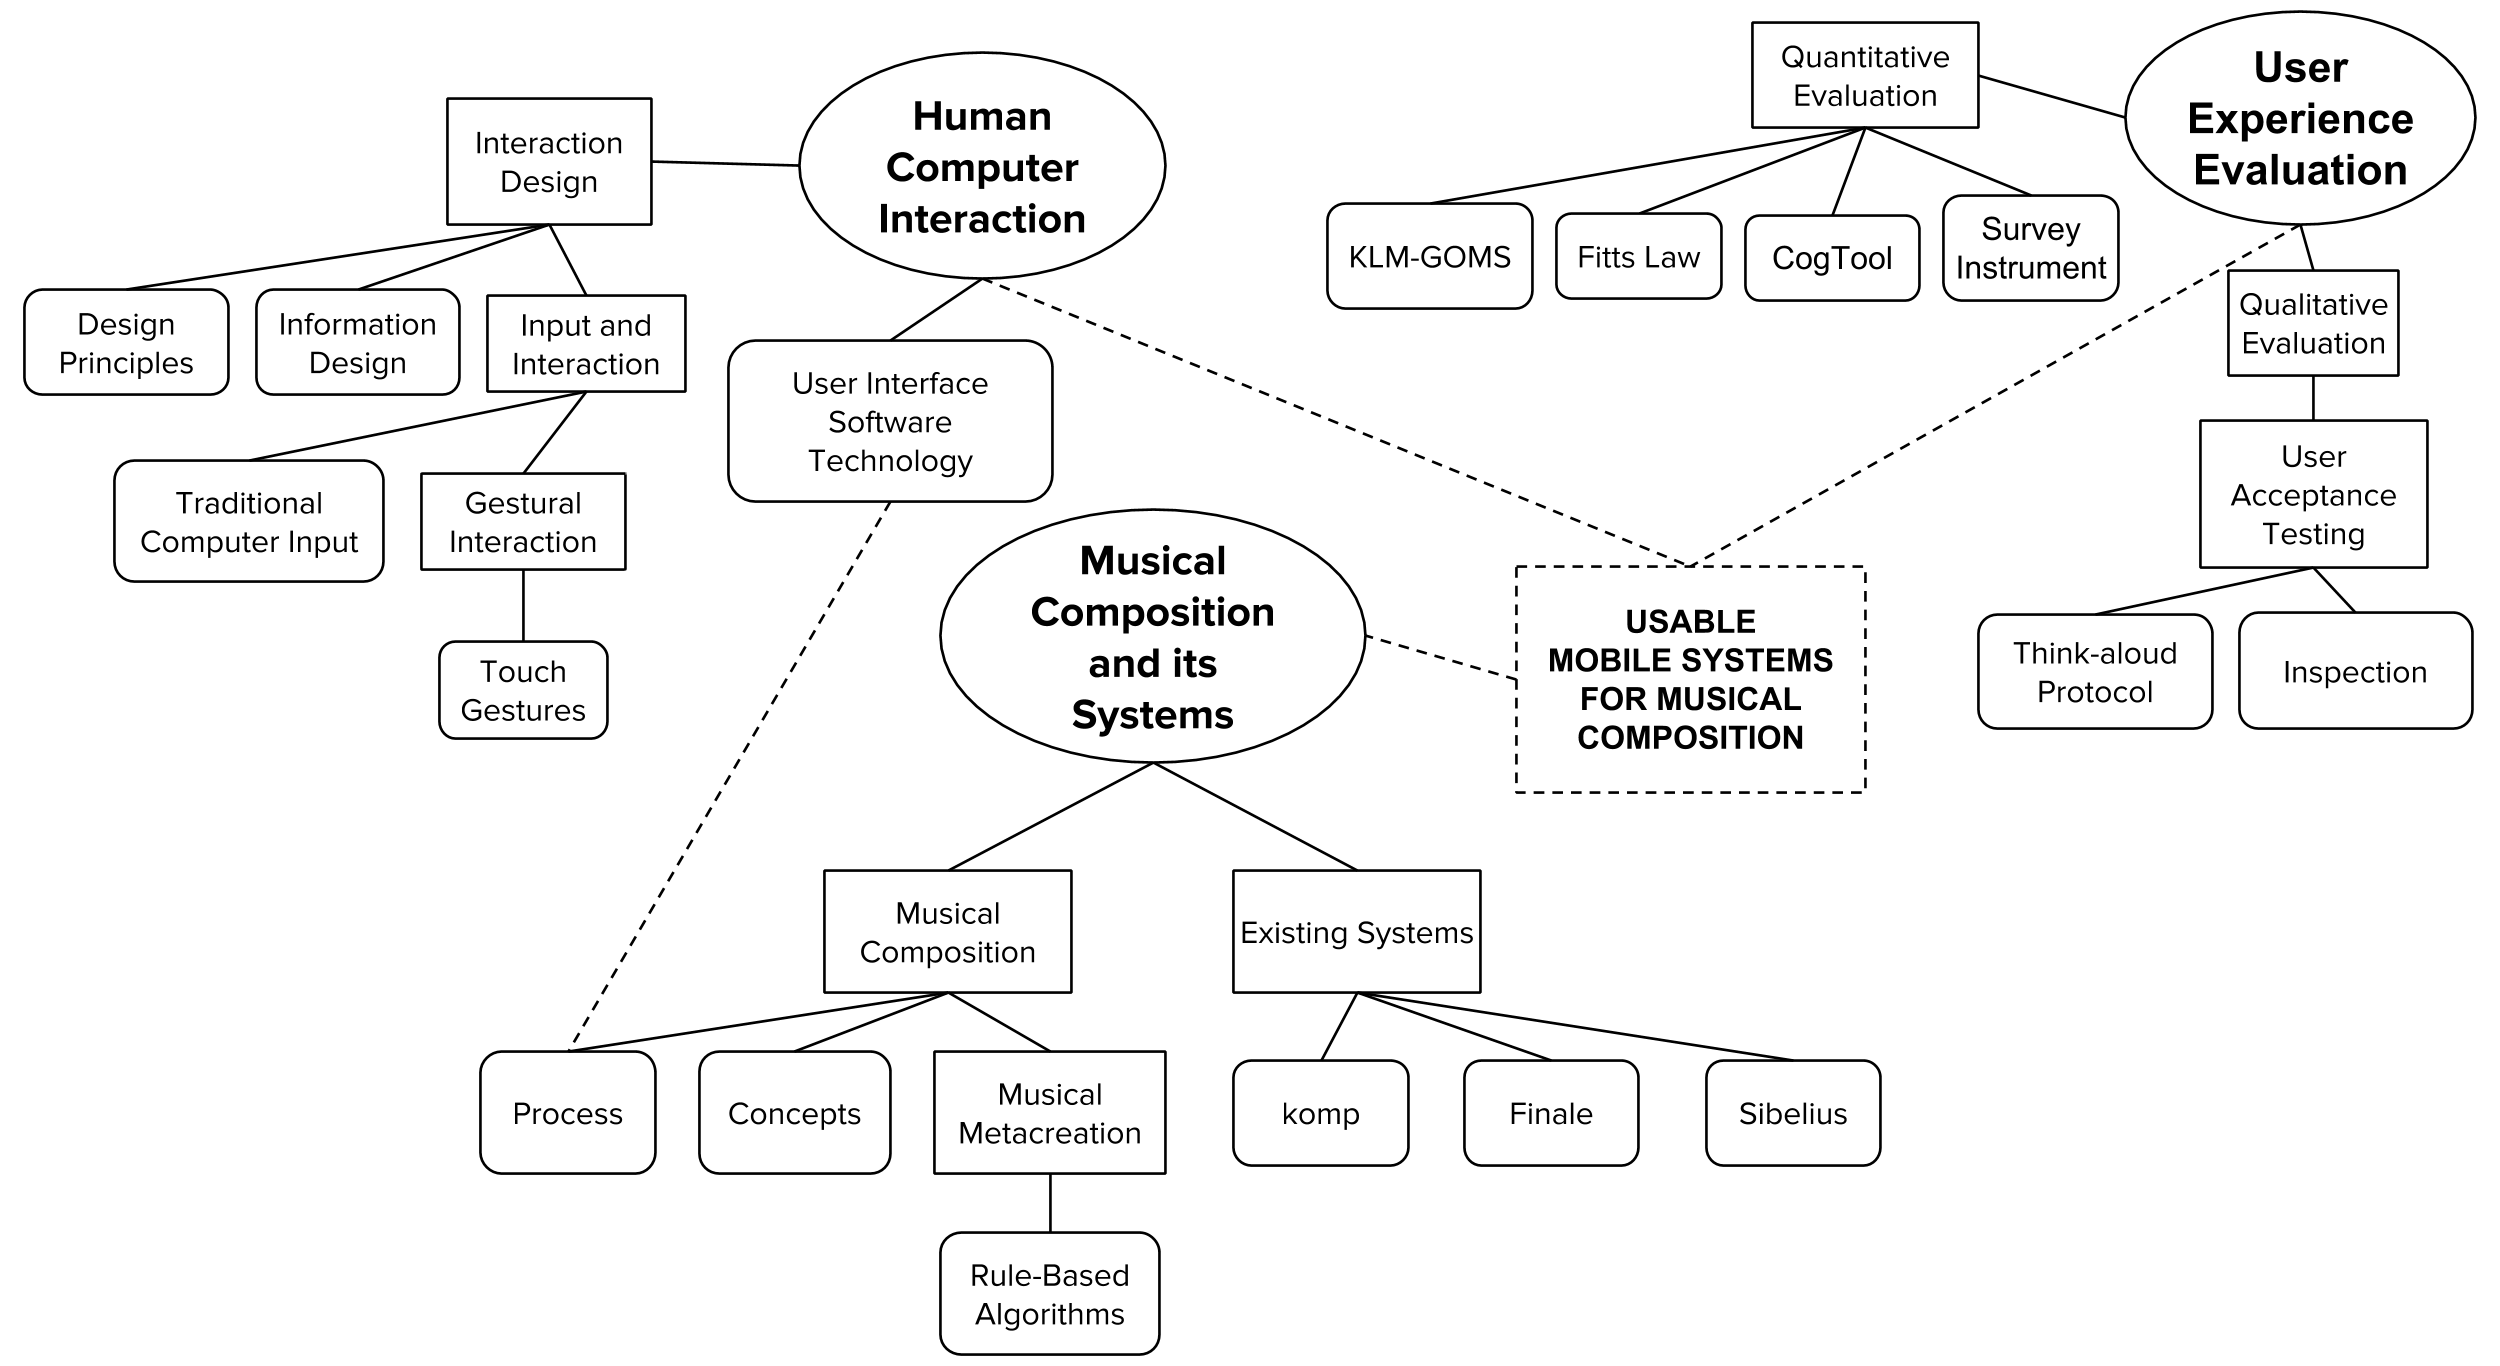
\includegraphics[scale=0.26]{literature_map}
      \caption{Literature map.}
      \label{fig:literature-map}
  \end{sidewaysfigure}

\chapter{User Personas}
\label{sec:user-personas}

  \begin{comment}
  \begin{wrapfigure}{l}{0.5\textwidth}

    \begin{center}
      
\includegraphics[width=0.48\textwidth]{mary_persona}
    \end{center}
  \end{wrapfigure}
  \end{comment}

  \subsection{Mary: The Amateur}

  \begin{itemize}
  \item 18 years old
  \item Started composing as a hobby when she was 16 years old
  \item 2nd Year undergraduate student
  \item Currently taking up a Bachelor in Music degree program
  \item Passing grades during her 1st Year
  \end{itemize}

  "Its such a hassle to write notes on music sheets. Its hard to keep track which are the drafts."

  "I haven't found any app like Finale in the app store."

  Mary lives in a dorm with 3 other people and has her own laptop and tablet. She uses both of these devices to do her work in any place.

  Mary mostly uses music sheets when she needs to compose music for assignments. She usually uses her laptop for research and the tablet as a substitute when she doesn't feel like bringing her laptop.

  Mary has passing marks in her courses. She experiences difficulty getting high grades because she has a hard time looking for inspiration and ideas. She also easily gets tired writing, revising, and finalizing her compositions on paper.

  She is knowledgeable in using Sibelius on her laptop and has started to learn Finale due to her professors urging her to use it. She appreciates how these kinds of applications reduce the steps in some repetitive or tedious processes in composing music.

  \begin{comment}
  \begin{wrapfigure}{l}{0.5\textwidth}
    \begin{center}
    
      
\includegraphics[width=0.48\textwidth]{warren_persona}
    \end{center}
  \end{wrapfigure}
  \end{comment}

  \subsection{Warren: The Experienced}

  \begin{itemize}
  \item 34 years old
  \item 10 years of composing music professionally
  \item Music teacher in a high school
  \item Loves classical music
  \item Music fundamentalist
  \item Wants his students to be more engaged in music and appreciate the art form
  \item Faculty for 5 years
  \end{itemize}

  "Music is a way to truly express yourself"

  "I want to share my passion in music to my pupils"

  Warren is currently a faculty member of a private high school that pays him enough that he can make a living and support his family.

  Warren has been teaching for 5 years. He has been involved in organizing the curriculum in the school. He has always believed that music as an art form is timeless and should be learned by everyone.

  He wants his students to appreciate music as much as he does. He shares the works of Beethoven and Mozart, which are his favorites, to his class.

  % He wants his students to appreciate music since years of hard work from various authors like Beethoven and Mozart have devoted their whole lives to the art. 

  He often observes students using their mobile devices in school. During class, he's made it clear that the usage of cellphones is restricted. However, he understands the potential of these mobile devices as tools for musical composition.

  % He often observes students being too distracted with their devices in school. During class, he's made it clear that the usage of cellphones is restricted. Though, he can see the usefulness of the technology for research and some classes in his school has integrated e-learning.

  He is experienced in using Finale but still uses music sheets during occasions where he cannot use his laptop or is still sketching. He has been wondering whether there is a viable mobile alternative to using music sheets.

  % He's been wondering if these technologies can be used for teaching music but he's on the fence about it because students might not experience music fully.


  \begin{comment}
  \begin{wrapfigure}{l}{0.5\textwidth}
    \begin{center}
      
\includegraphics[width=0.48\textwidth]{winston_persona}
    \end{center}
  \end{wrapfigure}
  \end{comment}

  \subsection{Winston: The Veteran}

  \begin{itemize}
  \item 62 Years Old
  \item 40 years of experience in composing music professionally
  \item Composes music for different companies and artists
  \item Mentors up and coming composers
  %\item Active in international conferences about the field of Music
  \item Married for 35 years
  \item Has experienced the numerous shifts of popularity between music genres
  \end{itemize}

  "Music has always been a part of everyone's lives" 

  "I wonder whats next the next big thing that can change music" 

  Warren always reads on music-related news and enjoys doing research on topics that concern music. He writes his findings and his thoughts on his blog. He has lived through several shifts in mainstream music and has studied the change agent in every shift. 

  He has been able to adjust and make a living from these hobbies. He has always been able to make music that matched what was popular at the time. He fully accepts that music changes for every new generation of artists and composers.

  He is waiting for the next big thing that can happen for music, always prepared to make the needed adjustments to stay in the game. He is no stranger to using technology like Finale or Sibelius to compose his pieces.

\begin{comment}
\chapter{Resource Persons}
\label{sec:appendixf}

\newcommand{\resperson}[4]{\textbf{#1} \\ #2 \\ #3 \\ \url{#4}\vspace{0.5em}\\}

\resperson{Mr. Jordan Aiko Deja}{Adviser}{College of Computer Studies\\De La Salle University-Manila}{jordan.deja@dlsu.edu.ph}
\\
\resperson{Dr. Rafael Cabredo}{Chair, Software Technology Department}{College of Computer Studies\\De La Salle University-Manila}{rafael.cabredo@dlsu.edu.ph}

\end{comment}

\chapter{User Stories}
\label{sec:user_stories}

  The user stories of the system will be focused on the main functions of the application and will highlight each specific need that the user has for the system. These user stories came from identified user needs, representing the tasks that they need to perform on musical composition applications. These are created with the context that the system will run on a mobile platform with the mode of interaction mainly being touch gestures. 

  \begin{itemize}
    \item As a user, I want to be able to create a blank composition, so that I can start my work
    \item As a user, I want to be able to name my composition, so that I can differentiate it from my other compositions
    \item As a user, I want to be able to save my composition, so that I can come back to it later
    \item As a user, I want to be able to view all my saved compositions in a list, so that I can keep track of everything
    \item As a user, I want to be able to open a saved composition so that I can perform more actions on it
    \item As a user, I want to be able export my composition in a format that I can open in the composition application I use on my laptop
    \item As a user, I want to be able to delete a composition, so I can discard compositions I do not work on anymore
    \item As a user, I want to be able to place a note in my composition, so that I can create my composition
    \item As a user, I want to be able to select a note, so that I can perform actions on it
    \item As a user, I want to be able to change the pitch of a note in my composition, so that I can make adjustments to my composition
    \item As a user, I want to be able to change the type of a note in my composition, so that I can make the sound longer or shorter
    \item As a user, I want to be able to erase a note in my composition, so that I can make space for other notes in my composition
    \item As a user, I want to be able to highlight a group of notes in my composition, so that I can perform actions on the group
    \item As a user, I want to be able to erase a highlighted group of notes in my composition, so that I can make large changes faster
    \item As a user, I want to be able to place a rest in my composition, so I can have pauses in my composition
    \item As a user, I want to be able to select a rest, so that I can perform actions on that rest
    \item As a user, I want to be able to change the type of rest, so that I can change the length of pauses
    \item As a user, I want to be able to highlight a group of rests, so that I can perform actions on the group of rests
    \item As a user, I want to be able to erase a rest in my composition, so that I can make space for other rests or notes
    \item As a user, I want to be able to erase a highlighted group of rests in my composition, so that I can make large changes faster
    \item As a user, I want to be able to change a rest in my composition, so that I can make adjustments to my composition
    \item As a user, I want to be able to highlight a mixed group of notes and rests in my composition, so that I can perform actions on the group
    %\item As a user, I want to be able to move the position of a note in my composition, so that I can move that note to a better position
    %\item As a user, I want to be able to move the position of a highlighted group of notes in my composition, so that I can reposition multiple notes at a time to a better position
    \item As a user, I want to be able to hear the sound of the note I just added, so that I know I've added the correct sounding note
    %\item As a user, I want to be able to listen to a highlighted section of my composition, so that I can hear just a segment of my piece
    \item As a user, I want to be able to listen to my whole composition, so that I can hear it as a whole
    %\item As a user, I want to be able to perform a swipe gesture that will generate a succession of notes based on the orientation of my gesture and my current composition because I'm interested in knowing what series of notes match my current composition
    %\item As a user, I want to be able to manipulate the generated series of notes, because the generated series of notes just needs a little bit more adjustments before I accept it into my composition
    %\item As a user, I want to be able to discard the series of notes generated by the application after a swipe gesture, so I do not have to delete them one by one
    %\item As a user, I want to be able to confirm the addition of the series of notes given by the application after a swipe gesture, so I can create my composition quickly
    \item As a user I want to be able to undo an action or a series of actions, so that I can undo an unintended action or series of unintended actions quicker
    \item As a user I want to be able to redo an action or a series of actions, so that I can redo an intended action or a series of intended actions quicker
    \item As a user, I want to be able to reposition the menu because I want to place it where it is not an obstacle for me while composing
    %\item As a user, I want to be able to see the details of a single note, so that I can know the specifications of the note
    %\item As a user, I want to be able to see the details of a selected group of notes, so that I can know the specification of the selected group of notes
    %\item As a user, I want to be able to see the details of the generated series of notes like the pitch and type so that I can know what notes the system has generated after a gesture
    \item As a user, I want to be able to set the clef of my composition
    \item As a user, I want to be able to set the key signature of my composition
    \item As a user, I want to be able to set the time signature of my composition
    \item As a user, I want to be able to copy a highlighted group of notes and/or rests, so that I can copy a recurring segment in my composition
    \item As a user, I want to be able to cut a highlighted group of notes and/or rests, so that I can easily move a segment of my composition
    \item As a user, I want to be able to paste the copied or cut group of notes and/or rests onto my composition, so that I do not need to add a recurring segment in my composition manually all the time
    %\item As a user, I want to be able to move the position of a rest, so that I can move that rest to a better position
    %\item As a user, I want to be able to move the position of a selected group of rests, so that I can move multiple rests at a time to a better position
    \item As a user, I want to be able to add accidentals to my notes, so that I can control the pitch of my notes
    \item As a user, I want to be able to remove accidentals from my notes, so that I can control the pitch of my notes
    \item As a user, I want to be able to add ottavas and ottava bassas on my notes, so that I can easily change the octave of my notes
    \item As a user, I want to be able to remove ottavas and ottava bassas on my notes, so that I can easily change the octave of my notes
    \item As a user, I want to be able to transpose a highlighted group of notes, so that I do not need to individually change the pitch of each note
    \item As a user, I want to be able to perform retrograde inversion on a group of notes, so that I do not need to invert each note individually
  \end{itemize}

\chapter{Use Cases}

  This chapter defines the several actions the users can perform within the system. These use cases were derived from the needs of the composers and the functions of Flow. The design of each use case will be based on fully dressed use cases with precision level 2 found in the book of \cite{alistair2001writing}. The headers in each use case will be: trigger, primary actor, supporting actors, preconditions, minimal guarantees, success guarantees, and process steps.

  \textbf{Trigger} \\
  The main situation or goal that the use case will be revolving around. 

  \textbf{Primary Actor} \\
  The main entity that will be performing or influencing situation or goal directly.

  \textbf{Supporting Actors} \\
  Additional entities that will be indirectly or directly influenced by the outcome of the situation. These entities can also be influencing the decision making or performance of the primary actor.

  \textbf{Preconditions} \\
  These conditions need to be followed before the process steps can be performed.

  \textbf{Process Steps} \\
  Each step will be performed by the primary actor to accomplish the goal.

  \textbf{Minimal Guarantees} \\
  Outcome or result that will occur in case a goal is not fully accomplished.

  \textbf{Success Guarantees} \\
  Outcome or result that occurs when a goal is fully accomplished.

  %Trigger
  %Primary Actor
  %Supporting Actors
  %Precondition
  %Process Steps
  %Minimal Guarantees
  %Success Guarantees


  %%Layout needs to be fixed

  %Sprint 1
  \section{Use Case 1: Add a Single Note}

  \LTXtable{\textwidth}{longtables/use_case_1_lt}

  %Sprint 1
  \section{Use Case 2: Change a Single Note}

  \LTXtable{\textwidth}{longtables/use_case_2_lt}

  %Sprint 1
  \section{Use Case 3: Delete a Single Note through the Side Menu}

  \LTXtable{\textwidth}{longtables/use_case_3_lt}

  \section{Use Case 4: Delete a Single Note through a Flick Gesture}

  \begin{tabularx}{\textwidth}{|X|X|}
  \hline
  Trigger & 
  The composer needs to delete a note quickly \\
  \hline
  Primary Actor & 
  Composer\\
  \hline
  Supporting Actors & 
  \begin{itemize}
  \item Listener
  \item Instrumentalist
  \item Producer
  \item Flow
  \end{itemize} \\
  \hline
  Precondition & 
  \begin{itemize}
  \item The user has a composition open in Flow 
  \item The deletion of the selected note is valid based on the set musical rules
  \end{itemize} \\
  \hline
  Process Steps & 
  \begin{enumerate}
  \item The user performs a flick gesture on the note to be deleted
  \item Flow removes the selected note from the composition
  \end{enumerate} \\
  \hline
  Minimal Guarantees & 
  \begin{itemize}
    \item A note will be deleted
    \item The side menu will return to being transparent
  \end{itemize} \\
  \hline
  Success Guarantees & 
  \begin{itemize}
    \item The selected note will be deleted
    \item The space occupied by the selected note will be freed
  \end{itemize} \\
  \hline
  \end{tabularx}

  \section{Use Case 5: Toggle Accidental Marks on Note Addition}

  \LTXtable{\textwidth}{longtables/use_case_5_lt}

  \section{Use Case 6: Transform a Note to its Dotted Version}

  \LTXtable{\textwidth}{longtables/use_case_6_lt}

  \section{Use Case 7: Horizontal Swipe Gesture to Generate a Series of Notes}

  \LTXtable{\textwidth}{longtables/use_case_7_lt}

  \section{Use Case 8: Delete a Highlighted Group of Notes or Rests}

  \LTXtable{\textwidth}{longtables/use_case_8_lt}

  \section{Use Case 9: Replace a Highlighted Group of Notes or Rests with a Single Note}

  \LTXtable{\textwidth}{longtables/use_case_9_lt}

  \section{Use Case 10: Replace a Highlighted Group of Notes or Rests with a Single Rest}

  \LTXtable{\textwidth}{longtables/use_case_10_lt}


  \section{Use Case 11: Single Note Transposition}

  \begin{tabularx}{\textwidth}{|X|X|}
  \hline
  Trigger & 
  The user needs to transpose a note to set its pitch higher \\
  \hline
  Primary Actor & 
  Composer \\
  \hline
  Supporting Actors & 
  \begin{itemize}
  \item Listener
  \item Instrumentalist
  \item Producer
  \item Flow
  \end{itemize} \\
  \hline
  Precondition & 
  \begin{itemize}
  \item The user has a composition open in Flow
  \item The transposition is valid based on the set musical rules
  \end{itemize} \\
  \hline
  Process Steps & 
  \begin{enumerate}
  \item The user performs a two finger swipe gesture upwards on the desired note
  \item Flow increases the pitch of the note
  \end{enumerate} \\
  \hline
  Minimal Guarantees & 
  \begin{itemize}
    \item None
  \end{itemize} \\
  \hline
  Success Guarantees & 
  \begin{itemize}
    \item The desired note will be transposed upwards
  \end{itemize} \\
  \hline
  \end{tabularx}

  \section{Use Case 12: Multiple Note Transposition}

  \begin{tabularx}{\textwidth}{|X|X|}
  \hline
  Trigger & 
  The user needs to transpose a group of note to set their pitch higher \\
  \hline
  Primary Actor & 
  Composer \\
  \hline
  Supporting Actors & 
  \begin{itemize}
  \item Listener
  \item Instrumentalist
  \item Producer
  \item Flow
  \end{itemize} \\
  \hline
  Precondition & 
  \begin{itemize}
  \item The user has a composition open in Flow
  \item The batch transposition is valid based on the set musical rules
  \end{itemize} \\
  \hline
  Process Steps & 
  \begin{enumerate}
  \item The user highlights a group of notes
  \item The user performs a two finger swipe gesture upwards on the highlighted group of notes
  \item Flow increases the pitch of the highlighted group of notes
  \end{enumerate} \\
  \hline
  Minimal Guarantees & 
  \begin{itemize}
    \item None
  \end{itemize} \\
  \hline
  Success Guarantees & 
  \begin{itemize}
    \item The highlighted group of notes will be transposed upwards
  \end{itemize} \\
  \hline
  \end{tabularx}


  \section{Use Case 13: Retrograde a Collection of Notes}

  \begin{tabularx}{\textwidth}{|X|X|}
  \hline
  Trigger & 
  The user needs to retrograde a collection of notes \\
  \hline
  Primary Actor & 
  Composer \\
  \hline
  Supporting Actors & 
  \begin{itemize}
  \item Listener
  \item Instrumentalist
  \item Producer
  \item Flow
  \end{itemize} \\
  \hline
  Precondition & 
  \begin{itemize}
  \item The user has a composition open in Flow
  \item The retrograde does not violate the set musical rules
  \end{itemize} \\
  \hline
  Process Steps & 
  \begin{enumerate}
  \item The user highlights a group of notes
  \item The user performs a two finger flick gesture horizontally on top of the collection of notes
  \item Flow retrogrades the collection of notes
  \end{enumerate} \\
  \hline
  Minimal Guarantees & 
  \begin{itemize}
    \item None
  \end{itemize} \\
  \hline
  Success Guarantees & 
  \begin{itemize}
    \item The collection of notes will be retrograded
  \end{itemize} \\
  \hline
  \end{tabularx}

  \section{Use Case 14: Invert a Collection of Notes}

  \begin{tabularx}{\textwidth}{|X|X|}
  \hline
  Trigger & 
  The user needs to invert a collection of notes \\
  \hline
  Primary Actor & 
  Composer \\
  \hline
  Supporting Actors & 
  \begin{itemize}
  \item Listener
  \item Instrumentalist
  \item Producer
  \item Flow
  \end{itemize} \\
  \hline
  Precondition & 
  \begin{itemize}
  \item The user has a composition open in Flow
  \item The inversion does not violate the set musical rules
  \end{itemize} \\
  \hline
  Process Steps & 
  \begin{enumerate}
  \item The user highlights a group of notes
  \item The user performs a two finger flick gesture vertically on top of the collection of notes
  \item Flow inverts the collection of notes
  \end{enumerate} \\
  \hline
  Minimal Guarantees & 
  \begin{itemize}
    \item None
  \end{itemize} \\
  \hline
  Success Guarantees & 
  \begin{itemize}
    \item The collection of notes will be inverted
  \end{itemize} \\
  \hline
  \end{tabularx}

  \section{Use Case 15: Add a Chord}

  \LTXtable{\textwidth}{longtables/use_case_15_lt}

  \section{Use Case 16: Add a Single Rest}

  \LTXtable{\textwidth}{longtables/use_case_16_lt}

  \section{Use Case 17: Change a Single Rest}

  \LTXtable{\textwidth}{longtables/use_case_17_lt}

  %Sprint 1
  \section{Use Case 18: Delete a Single Rest through the Side Menu}

  \LTXtable{\textwidth}{longtables/use_case_18_lt}


  \section{Use Case 19: Delete a Single Rest through Flick Gesture}

  \begin{tabularx}{\textwidth}{|X|X|}
  \hline
  Trigger & 
  The composer needs to delete a rest quickly \\
  \hline
  Primary Actor & 
  Composer\\
  \hline
  Supporting Actors & 
  \begin{itemize}
  \item Listener
  \item Instrumentalist
  \item Producer
  \item Flow
  \end{itemize} \\
  \hline
  Precondition & 
  \begin{itemize}
  \item The user has a composition open in Flow 
  \item The deletion of the selected rest is valid based on the set musical rules
  \end{itemize} \\
  \hline
  Process Steps & 
  \begin{enumerate}
  \item The user performs a flick gesture on the rest to be deleted
  \item Flow removes the selected rest from the composition
  \end{enumerate} \\
  \hline
  Minimal Guarantees & 
  \begin{itemize}
    \item A rest will be deleted
    \item The side menu will return to being transparent
  \end{itemize} \\
  \hline
  Success Guarantees & 
  \begin{itemize}
    \item The selected rest will be deleted
    \item The space occupied by the selected rest will be freed
  \end{itemize} \\
  \hline
  \end{tabularx}

  \section{Use Case 20: Listen to a Single Note}

  \begin{tabularx}{\textwidth}{|X|X|}
  \hline
  Trigger & 
  The user needs to listen to a single note \\
  \hline
  Primary Actor & 
  Composer \\
  \hline
  Supporting Actors & 
  \begin{itemize}
  \item Listener
  \item Instrumentalist
  \item Producer
  \item Flow
  \end{itemize} \\
  \hline
  Precondition & 
  \begin{itemize}
  \item The user has a composition open in Flow
  \end{itemize} \\
  \hline
  Process Steps & 
  \begin{enumerate}
  \item The user selects a note
  \item The user taps on the play button
  \item Flow will play the sound of the selected note
  \end{enumerate} \\
  \hline
  Minimal Guarantees & 
  \begin{itemize}
   \item The icon for the play button will become a pause symbol then return to a play symbol once the composition is done playing
  \end{itemize} \\
  \hline
  Success Guarantees & 
  \begin{itemize}
    \item The selected note will be played
  \end{itemize} \\
  \hline
  \end{tabularx}

  \section{Use Case 21: Listen to a Highlighted Section of the Composition}

  \LTXtable{\textwidth}{longtables/use_case_21_lt}

  \section{Use Case 22: Listen to the Whole Composition}

  \begin{tabularx}{\textwidth}{|X|X|}
  \hline
  Trigger & 
  The user needs to listen to the whole composition \\
  \hline
  Primary Actor & 
  Composer \\
  \hline
  Supporting Actors & 
  \begin{itemize}
  \item Listener
  \item Instrumentalist
  \item Producer
  \item Flow
  \end{itemize} \\
  \hline
  Precondition & 
  \begin{itemize}
  \item The user has a composition open in Flow
  \item The composition is not empty
  \item The user has no notes selected or highlighted
  \end{itemize} \\
  \hline
  Process Steps & 
  \begin{enumerate}
  \item The user taps on the play button
  \item Flow will play the whole composition
  \end{enumerate} \\
  \hline
  Minimal Guarantees & 
  \begin{itemize}
    \item The icon for the play button will become a pause symbol then return to a play symbol once the composition is done playing
  \end{itemize} \\
  \hline
  Success Guarantees & 
  \begin{itemize}
    \item The whole composition will be played correctly until the last note or rest
  \end{itemize} \\
  \hline
  \end{tabularx}

  \section{Use Case 23: View the Details of a Single Note or Rest}

  \begin{tabularx}{\textwidth}{|X|X|}
  \hline
  Trigger & 
  The user needs to know the details of a single note or rest\\
  \hline
  Primary Actor & 
  Composer \\
  \hline
  Supporting Actors & 
  \begin{itemize}
  \item Listener
  \item Instrumentalist
  \item Producer
  \item Flow
  \end{itemize} \\
  \hline
  Precondition & 
  \begin{itemize}
  \item The user has a composition open in Flow
  \item The note or rest is in the composition
  \end{itemize} \\
  \hline
  Process Steps & 
  \begin{enumerate}
  \item The user selects a note or rest
  \item The user taps on the toggle details option
  \item Flow will display the details of the note or rest
  \end{enumerate} \\
  \hline
  Minimal Guarantees & 
  \begin{itemize}
    \item The toggle button graphic will change
  \end{itemize} \\
  \hline
  Success Guarantees & 
  \begin{itemize}
    \item The toggle button graphic will change
    \item The details of the selected note or rest will be displayed 
  \end{itemize} \\
  \hline
  \end{tabularx}


  \section{Use Case 24: View the Details of a Highlighted Group of Notes or Rests}

  \LTXtable{\textwidth}{longtables/use_case_24_lt}

  \section{Use Case 25: Copy and Paste a Single Note or Rest}

  \LTXtable{\textwidth}{longtables/use_case_25_lt}

  \section{Use Case 26: Cut and Paste a Single Note or Rest}

  \LTXtable{\textwidth}{longtables/use_case_26_lt}

  \section{Use Case 27: Copy and Paste a Group of Notes or Rests}

  \LTXtable{\textwidth}{longtables/use_case_27_lt}

  \section{Use Case 28: Cut and Paste a Group of Notes or Rests}

  \LTXtable{\textwidth}{longtables/use_case_28_lt}

  %Sprint 1
  \section{Use Case 29: Create Blank Composition}

  \LTXtable{\textwidth}{longtables/use_case_29_lt}

  %Sprint 1
  \section{Use Case 30: View Existing Composition}

  \begin{tabularx}{\textwidth}{|X|X|}
  \hline
  Trigger & 
  The user needs to view an existing composition \\
  \hline
  Primary Actor & 
  Composer \\
  \hline
  Supporting Actors & 
  \begin{itemize}
  \item Listener
  \item Instrumentalist
  \item Producer
  \item Flow
  \end{itemize} \\
  \hline
  Precondition & 
  \begin{itemize}
  \item The user is in the main menu screen
  \item The composition is in storage
  \item The composition is not corrupted
  \end{itemize} \\
  \hline
  Process Steps & 
  \begin{enumerate}
  \item The user taps on the composition from the main menu
  \item Flow opens the selected composition
  \end{enumerate} \\
  \hline
  Minimal Guarantees & 
  \begin{itemize}
    \item None
  \end{itemize} \\
  \hline
  Success Guarantees & 
  \begin{itemize}
    \item The selected composition will open
  \end{itemize} \\
  \hline
  \end{tabularx}

  %Sprint 1
  \section{Use Case 31: Delete Existing Composition}

  \begin{tabularx}{\textwidth}{|X|X|}
  \hline
  Trigger & 
  The user needs to delete a composition \\
  \hline
  Primary Actor & 
  Composer \\
  \hline
  Supporting Actors & 
  \begin{itemize}
  \item Listener
  \item Instrumentalist
  \item Producer
  \item Flow
  \end{itemize} \\
  \hline
  Precondition & 
  \begin{itemize}
  \item The user is in the main menu screen
  \item The composition is in storage
  \end{itemize} \\
  \hline
  Process Steps & 
  \begin{enumerate}
  \item The user taps on the delete composition button from the main menu
  \item The user taps confirm
  \item Flow deletes the selected composition
  \end{enumerate} \\
  \hline
  Minimal Guarantees & 
  \begin{itemize}
    \item None
  \end{itemize} \\
  \hline
  Success Guarantees & 
  \begin{itemize}
    \item The selected composition will be deleted
    \item Memory taken by the deleted composition will be freed
  \end{itemize} \\
  \hline
  \end{tabularx}

  \section{Use Case 32: Redo an Action}

  \begin{tabularx}{\textwidth}{|X|X|}
  \hline
  Trigger & 
  The user wants to redo an action\\
  \hline
  Primary Actor & 
  Composer \\
  \hline
  Supporting Actors & 
  \begin{itemize}
  \item Listener
  \item Instrumentalist
  \item Producer
  \item Flow
  \end{itemize} \\
  \hline
  Precondition & 
  \begin{itemize}
  \item An undo action has been performed at least once
  \item Redo action is valid based on the state of the composition
  \item Redo action is valid based on the set musical rules
  \end{itemize} \\
  \hline
  Process Steps & 
  \begin{enumerate}
  \item The user taps on the redo button
  \item Flow performs the undone action
  \end{enumerate} \\
  \hline
  Minimal Guarantees & 
  \begin{itemize}
    \item The redo button will give feedback 
  \end{itemize}\\
  \hline
  Success Guarantees & 
  \begin{itemize}
    \item The correct action is redone
  \end{itemize} \\
  \hline
  \end{tabularx}

  \section{Use Case 33: Undo an Action}

  \begin{tabularx}{\textwidth}{|X|X|}
  \hline
  Trigger & 
  The user wants to undo an action \\
  \hline
  Primary Actor & 
  Composer \\
  \hline
  Supporting Actors & 
  \begin{itemize}
  \item Listener
  \item Instrumentalist
  \item Producer
  \item Flow
  \end{itemize} \\
  \hline
  Precondition & 
  \begin{itemize}
  \item At least one action has been performed
  \item Undo action is valid based on the state of the composition
  \item Undo action is valid based on the set musical rules
  \end{itemize} \\
  \hline
  Process Steps & 
  \begin{enumerate}
  \item The user taps on the undo button
  \item Flow undos the last action
  \end{enumerate} \\
  \hline
  Minimal Guarantees & 
  \begin{itemize}
    \item The undo button will give feedback
  \end{itemize} \\
  \hline
  Success Guarantees & 
  \begin{itemize}
    \item The correct action is undone
  \end{itemize} \\
  \hline
  \end{tabularx}

  \section{Use Case 34: Select a Single Note or Rest}

  \begin{tabularx}{\textwidth}{|X|X|}
  \hline
  Trigger & 
  The user needs to select a note or rest \\
  \hline
  Primary Actor & 
  Composer \\
  \hline
  Supporting Actors & 
  \begin{itemize}
  \item Listener
  \item Instrumentalist
  \item Producer
  \item Flow
  \end{itemize} \\
  \hline
  Precondition & 
  \begin{itemize}
  \item The user has a composition open in Flow
  \end{itemize} \\
  \hline
  Process Steps & 
  \begin{enumerate}
  \item The user taps on a single note or rest
  \item Flow displays that the single note or rest is selected
  \end{enumerate} \\
  \hline
  Minimal Guarantees & 
  \begin{itemize}
    \item None
  \end{itemize} \\
  \hline
  Success Guarantees & 
  \begin{itemize}
    \item The look of a selected note or rest is differentiated from the unselected notes and rests
    \item The correct note or rest is selected
    \item Actions can be performed on the selected note or rest
  \end{itemize} \\
  \hline
  \end{tabularx}


  \section{Use Case 35: Highlight a Group of Notes or Rests}

  \LTXtable{\textwidth}{longtables/use_case_35_lt}

  \section{Use Case 36: Rename the Composition from the Composition Environment}

  \LTXtable{\textwidth}{longtables/use_case_36_lt}

  \section{Use Case 37: Rename the Composition from the Main Menu}

  \LTXtable{\textwidth}{longtables/use_case_37_lt}

  \section{Use Case 38: Move the Note Menu to a Different Position}

  \begin{tabularx}{\textwidth}{|X|X|}
  \hline
  Trigger & 
  The user needs to move the note menu to a different position\\
  \hline
  Primary Actor & 
  Composer \\
  \hline
  Supporting Actors & 
  \begin{itemize}
  \item Listener
  \item Instrumentalist
  \item Producer
  \item Flow
  \end{itemize} \\
  \hline
  Precondition & 
  \begin{itemize}
  \item The user has a composition open in Flow
  \item The new location for the note menu is valid
  \end{itemize} \\
  \hline
  Process Steps & 
  \begin{enumerate}
  \item The user drags the note menu to the desired location
  \item Flow will reposition the note menu during the drag gesture
  \end{enumerate} \\
  \hline
  Minimal Guarantees & 
  \begin{itemize}
    \item None
  \end{itemize} \\
  \hline
  Success Guarantees & 
  \begin{itemize}
    \item The note menu will move to its desired location
  \end{itemize} \\
  \hline
  \end{tabularx}

  \section{Use Case 39: Export to MusicXML from the Main Menu}

  \LTXtable{\textwidth}{longtables/use_case_39_lt}

  \section{Use Case 40: Toggle Notes to Rests to Chords in the Side Menu}

  \LTXtable{\textwidth}{longtables/use_case_40_lt}

  \section{Use Case 41: Change the Time Signature of the Composition}

  \LTXtable{\textwidth}{longtables/use_case_41_lt}

  \section{Use Case 42: Change the Key Signature of the Composition}

  \LTXtable{\textwidth}{longtables/use_case_42_lt}

  \section{Use Case 43: Change a Clef}

  \LTXtable{\textwidth}{longtables/use_case_43_lt}

\chapter{System Walkthrough}

\section{Main Menu}
The Main Menu (Figure \ref{fig:main-menu}) is the first screen shown to the user upon opening the application. This screen is where the user can create, open, export, and delete a composition. 

\section{Creating a Composition}
To create a new composition, the user may tap on the '+' icon which will lead to the Editor screen. 

\begin{figure}[H]
  \centering
  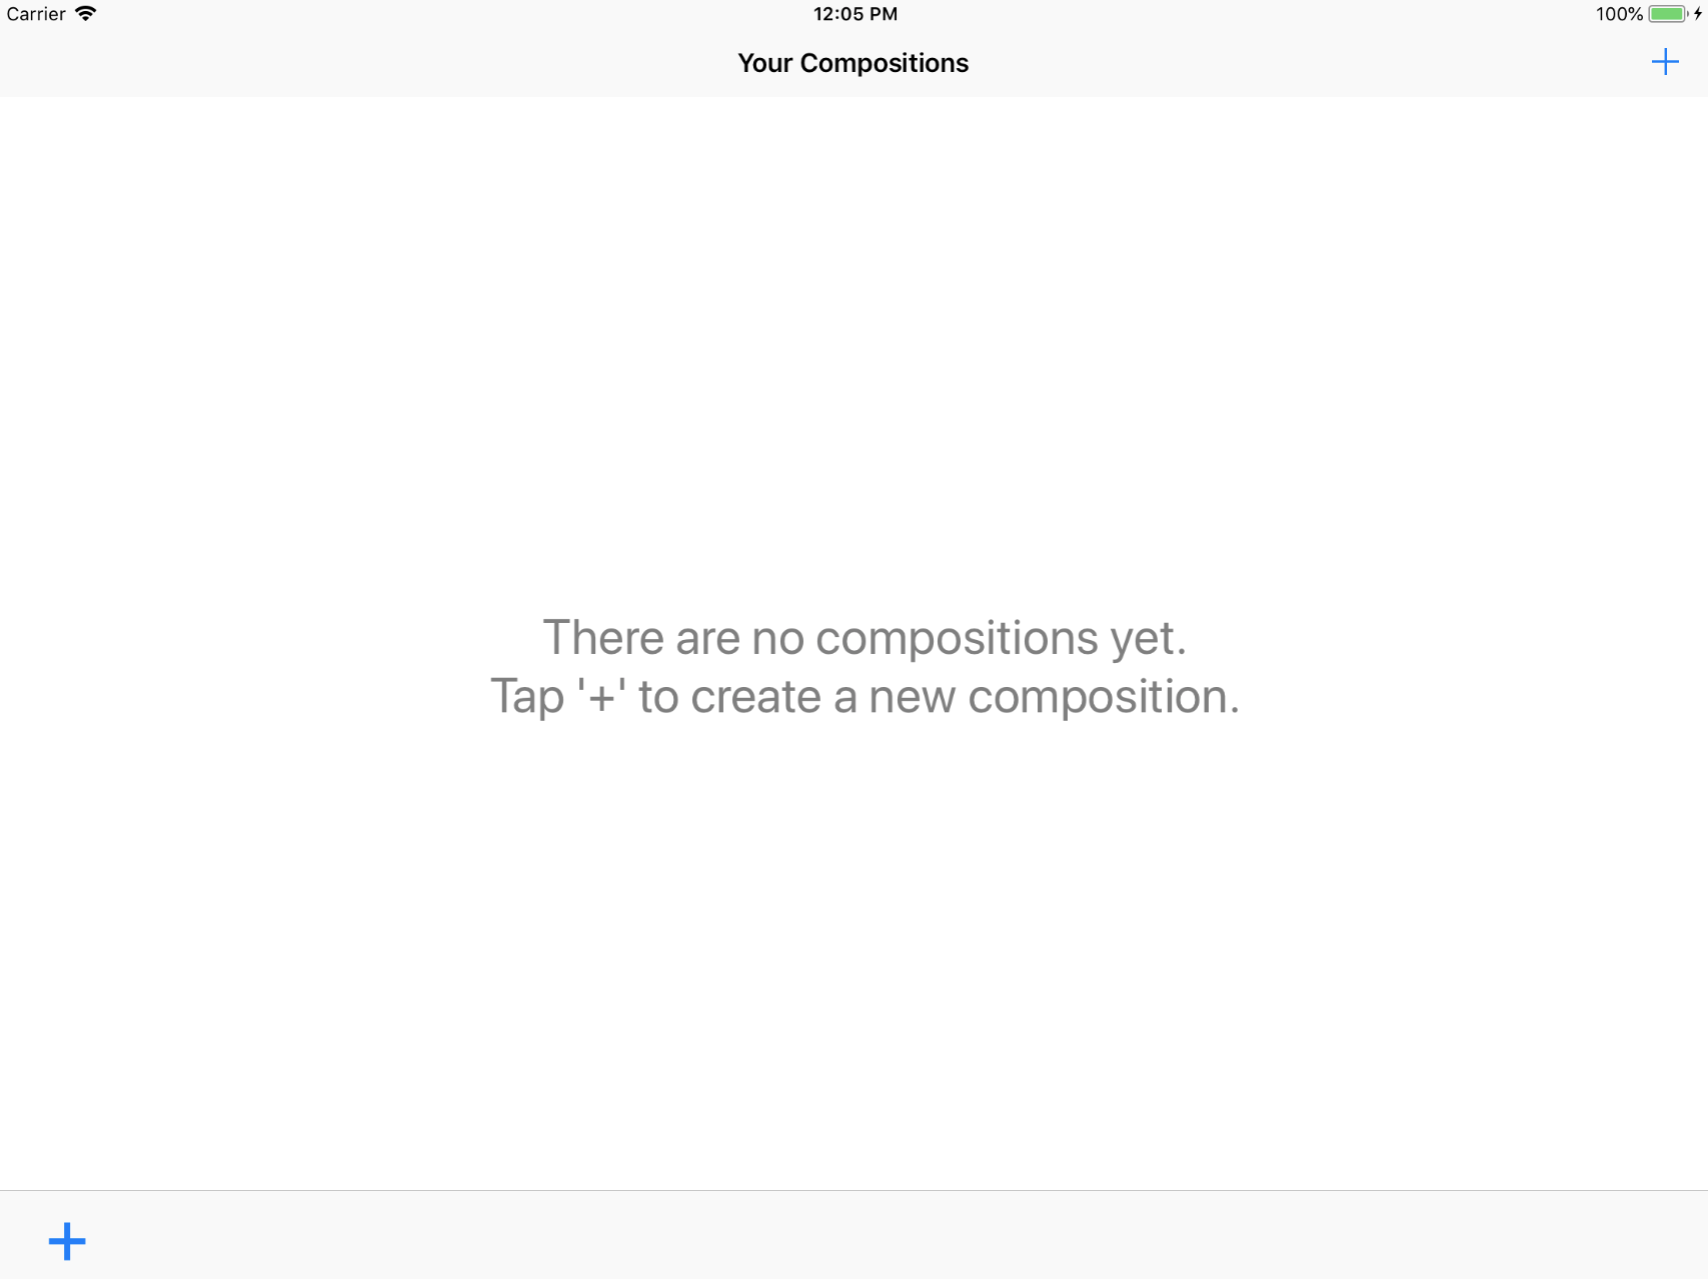
\includegraphics[scale=0.4]{Main_Menu}
    \caption{Flow Main Menu.}
    \label{fig:main-menu}
\end{figure}

\section{Opening a Composition}
Tapping an existing composition in the list will open it in the Editor screen allowing the user to edit. 

\section{Deleting, Renaming, and Exporting a Composition}
Swiping a composition to the left brings out the delete button (Figure \ref{fig:swipe-delete}). The user may also tap and hold an existing composition which brings out a modal for exporting (share), renaming, and deleting a composition (Figure \ref{fig:tap-hold-comp}).

\begin{figure}[H]
  \centering
  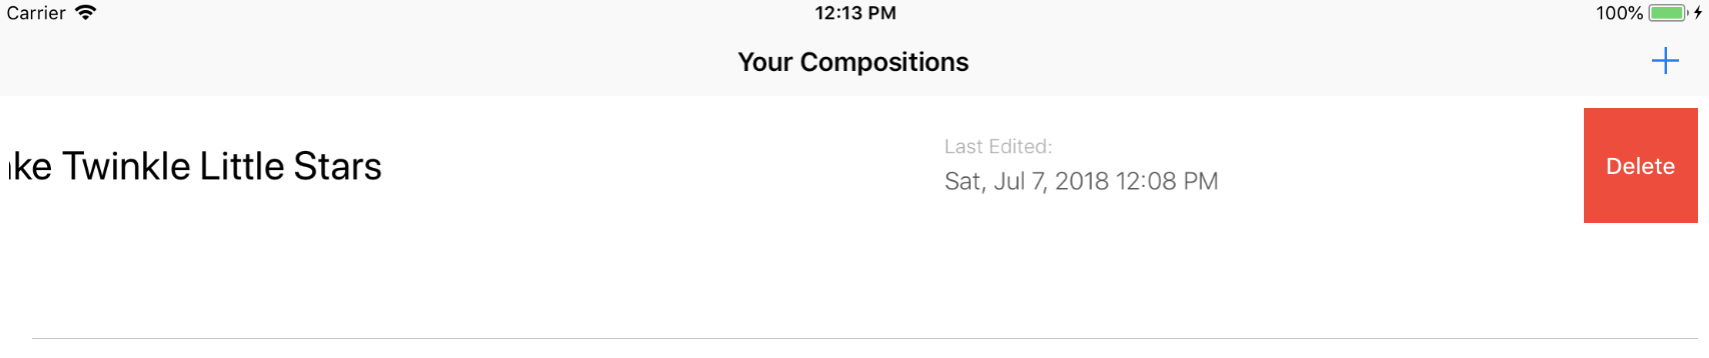
\includegraphics[scale=0.45]{Swipe_Delete}
    \caption{Swipe left to delete a composition.}
    \label{fig:swipe-delete}
\end{figure}

\begin{figure}[H]
  \centering
  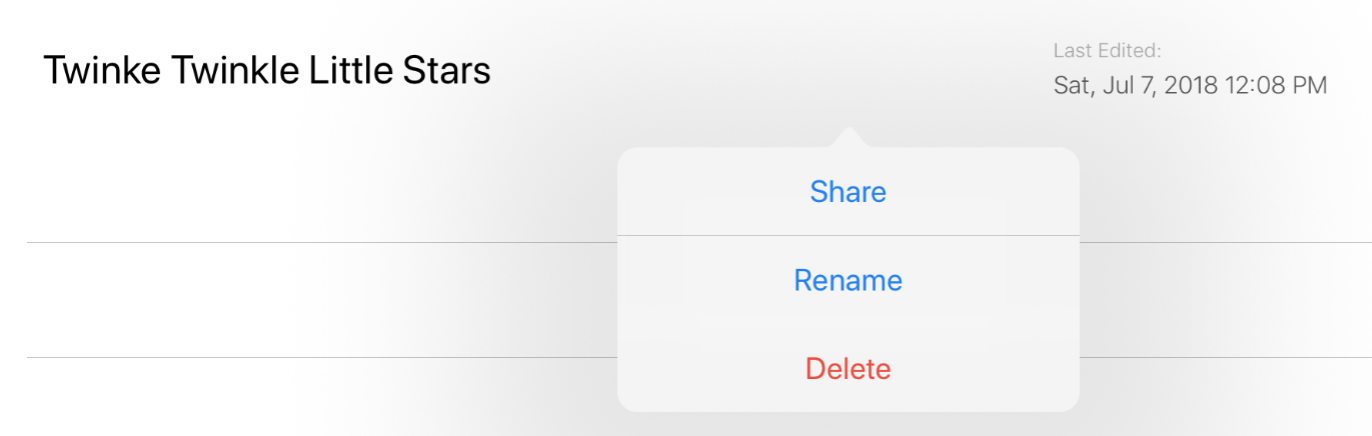
\includegraphics[scale=0.45]{Tap_And_Hold_Comp}
    \caption{Tap and hold a composition to bring out modal.}
    \label{fig:tap-hold-comp}
\end{figure}

\section{Editor}

The editor screen is where the user will spend most of the time using the application. It is where most of the composition process will take place. This includes adding, editing, and deleting of notes, rests and accidentals, setting the title, key signature, time signature, and tempo of the composition. This is also where the user can listen to the current progress of a composition through the playback functionality and also save a composition. Shown in Figure \ref{fig:editor} is the editor screen after creating a new composition from the main menu. 

\begin{figure}[H]
  \centering
  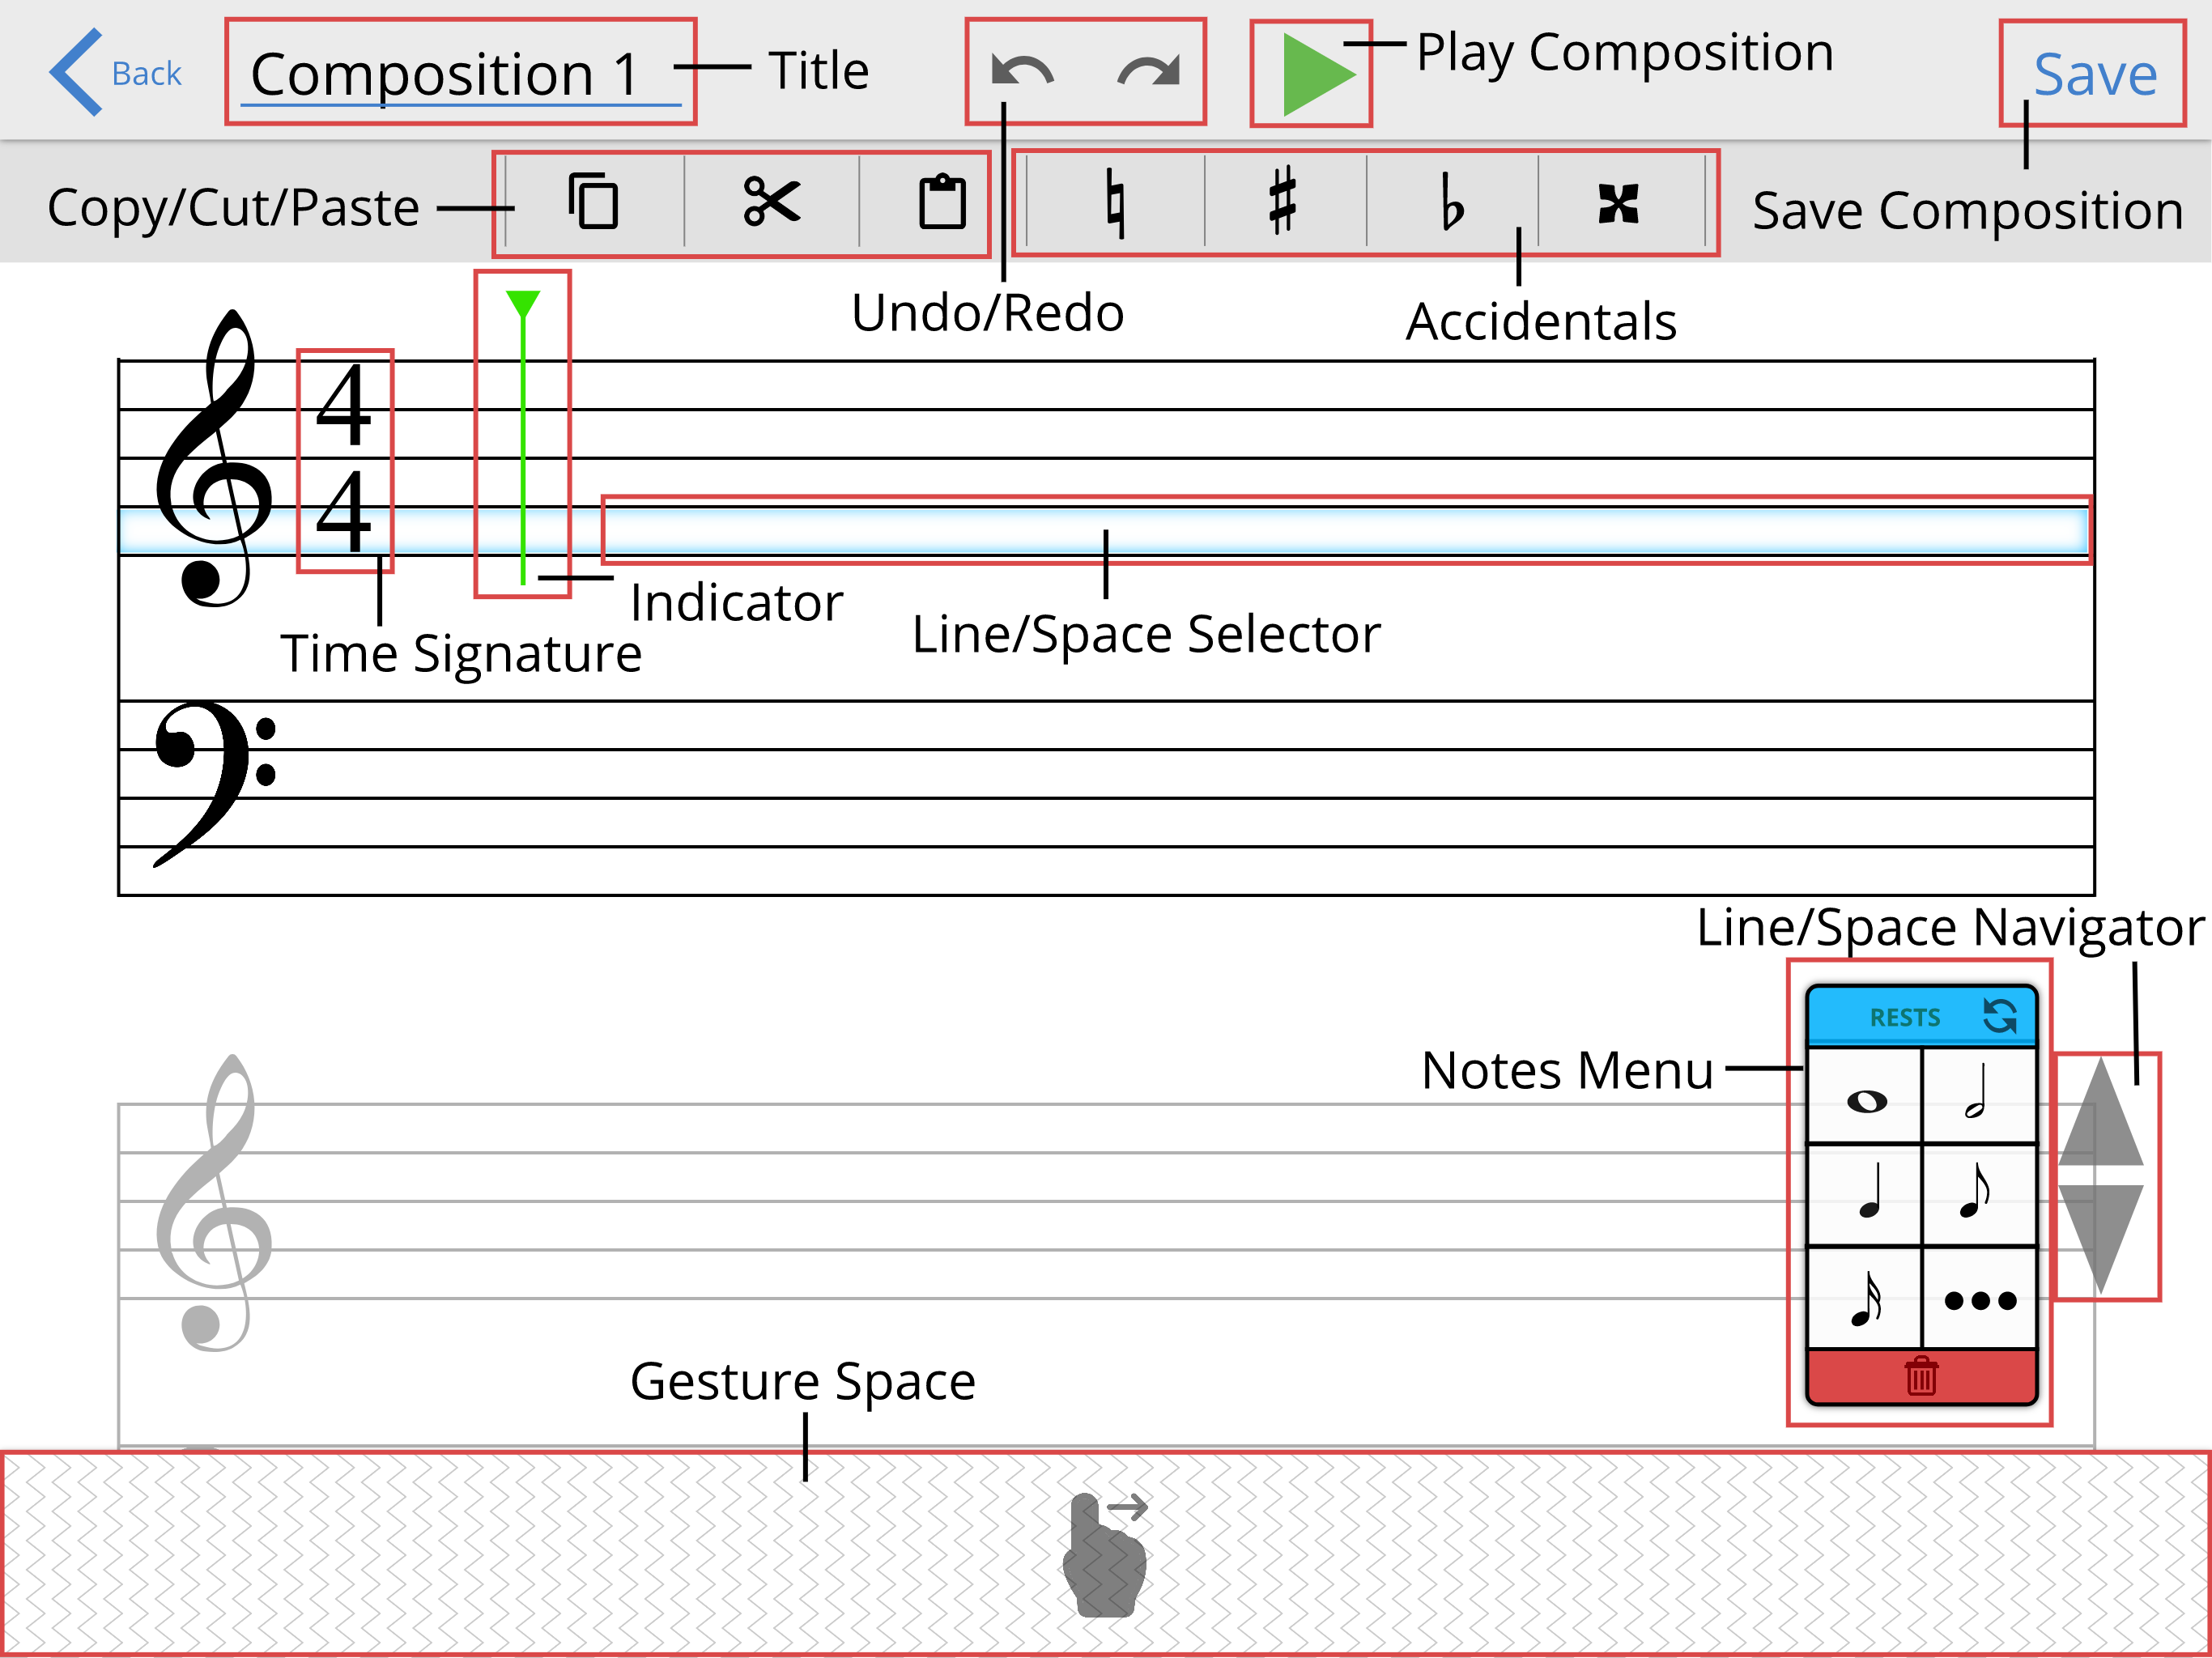
\includegraphics[scale=0.45]{Editor}
    \caption{Editor Screen.}
    \label{fig:editor}
\end{figure}

\section{Zooming and Panning}
To zoom out on the editor, the user must use the pinch in gesture (Figure \ref{fig:pinch-in}) and to zoom in, the user must use the pinch out gesture (Figure \ref{fig:pinch-out}). To pan the editor, the user must do a 2 finger drag gesture.

\begin{figure}[H]
  \centering
  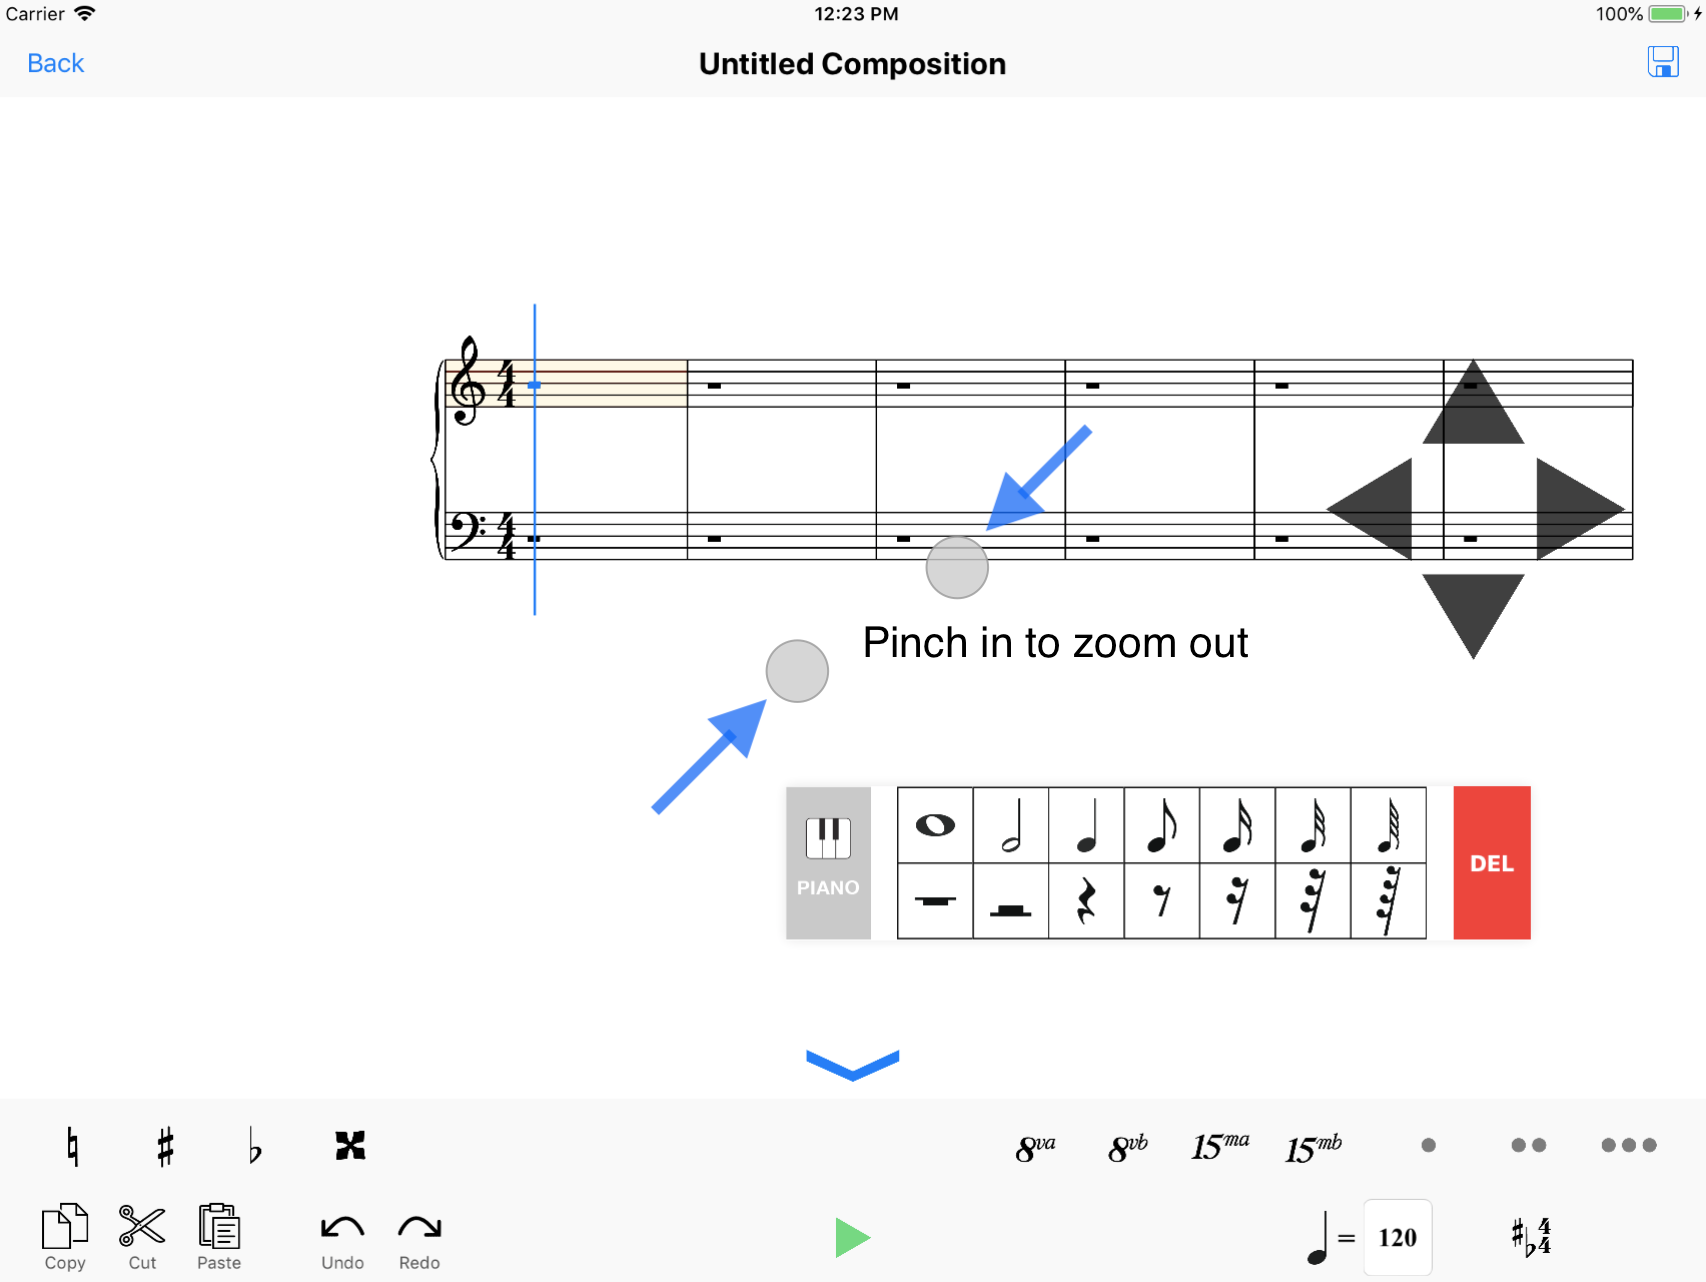
\includegraphics[scale=0.4]{Pinch_In}
    \caption{Pinch in to zoom out.}
    \label{fig:pinch-in}
\end{figure}

\begin{figure}[H]
  \centering
  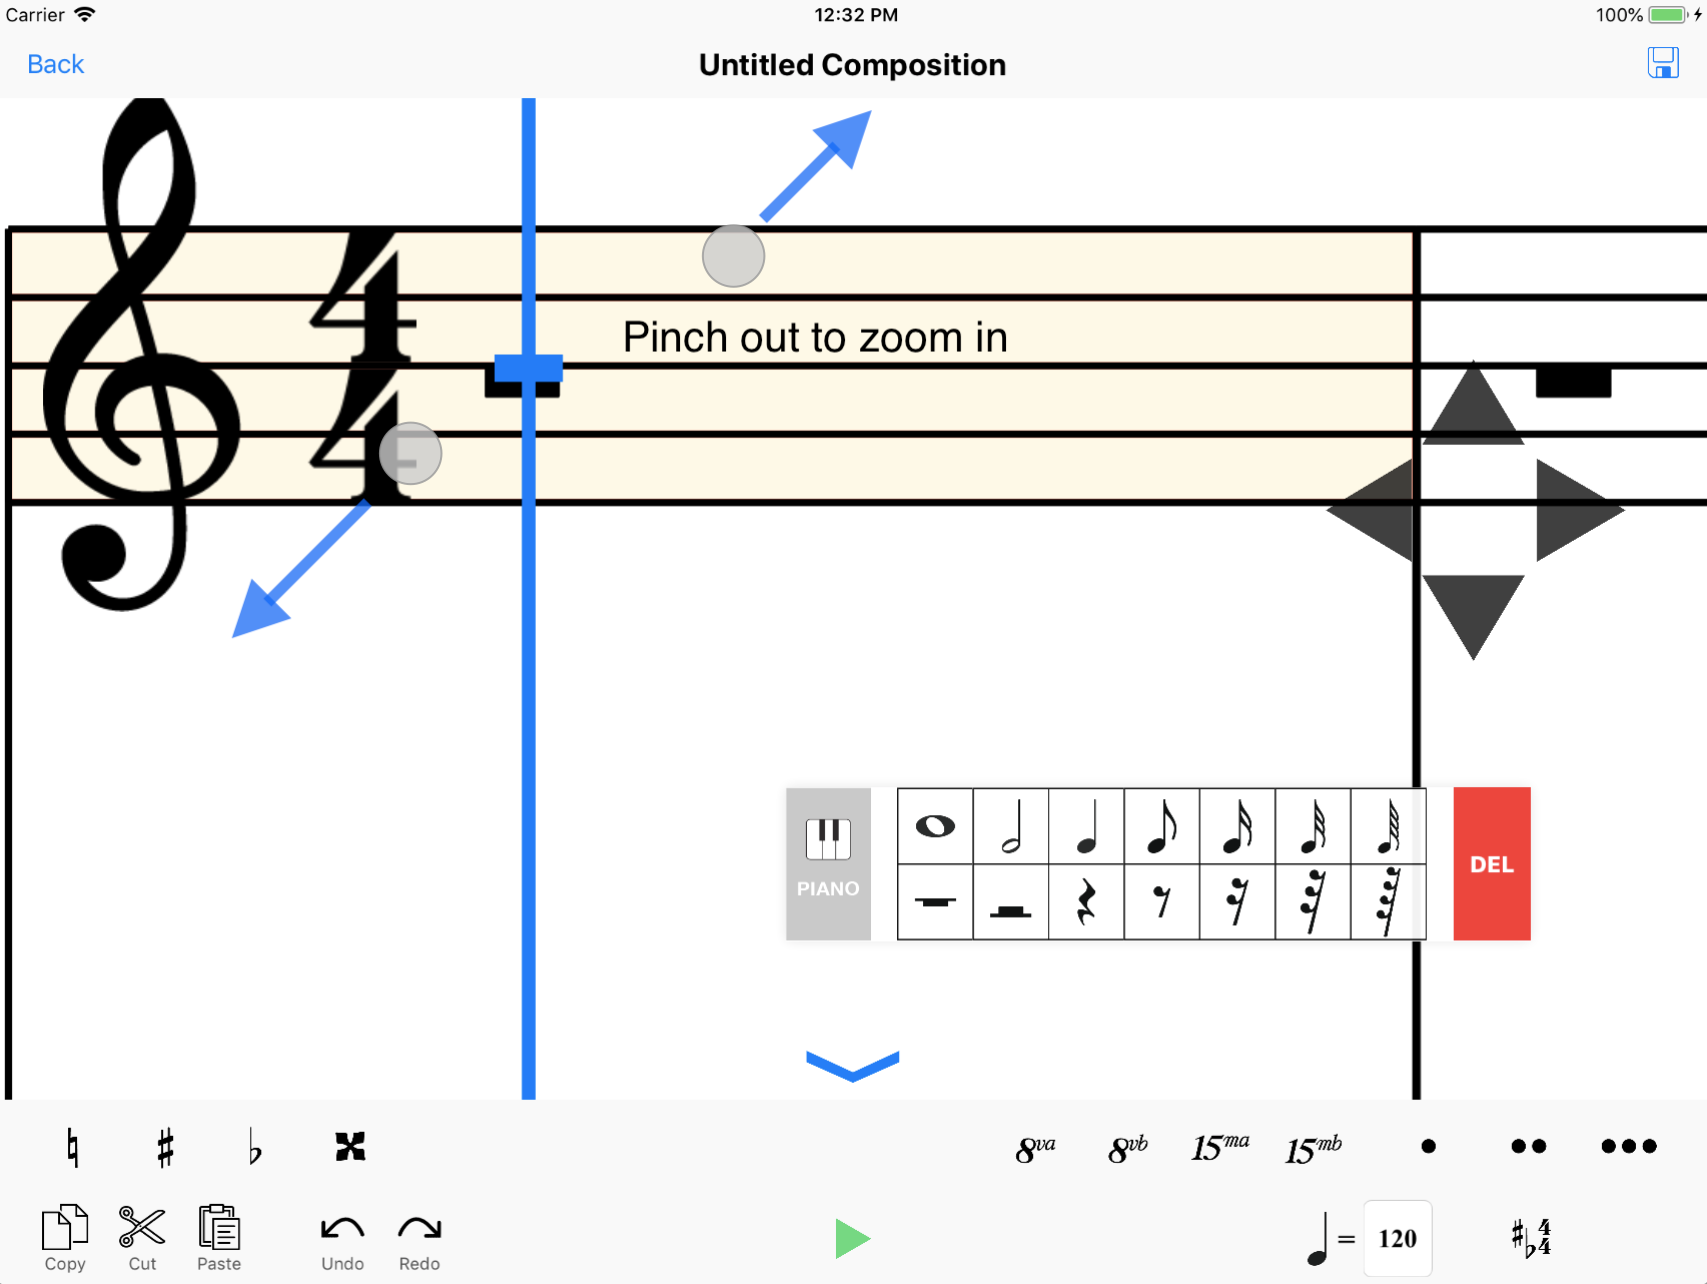
\includegraphics[scale=0.4]{Pinch_Out}
    \caption{Pinch out to zoom in.}
    \label{fig:pinch-out}
\end{figure}

\begin{figure}[H]
  \centering
  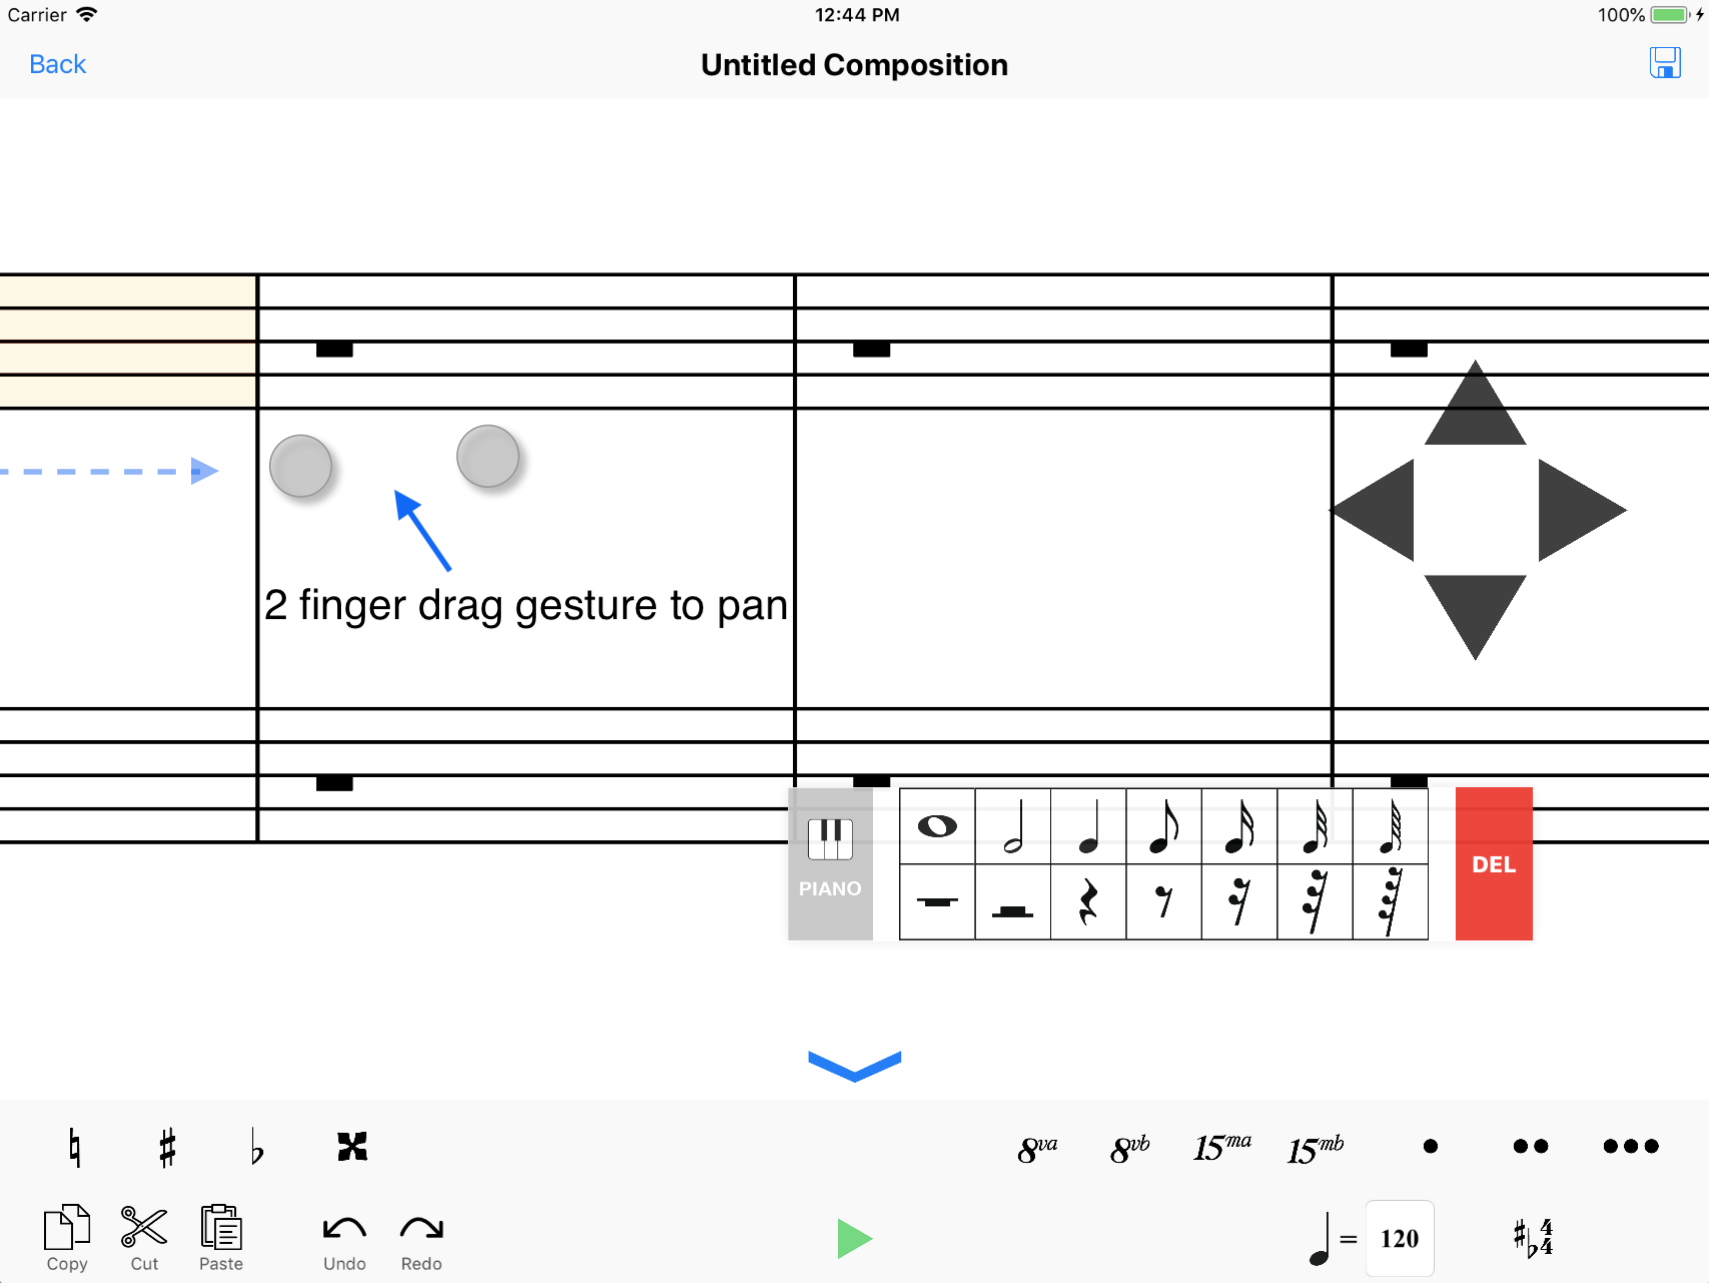
\includegraphics[scale=0.4]{Pan}
    \caption{Two finger drag gesture to pan.}
    \label{fig:pan}
\end{figure}

\section{Moving the Controls}
The controls in the editor such as the arrow controls and the notation controls are draggable views which allow the user to move them around for flexibility through a 1 finger drag gesture (Figure \ref{fig:move-controls}).

\begin{figure}[H]
  \centering
  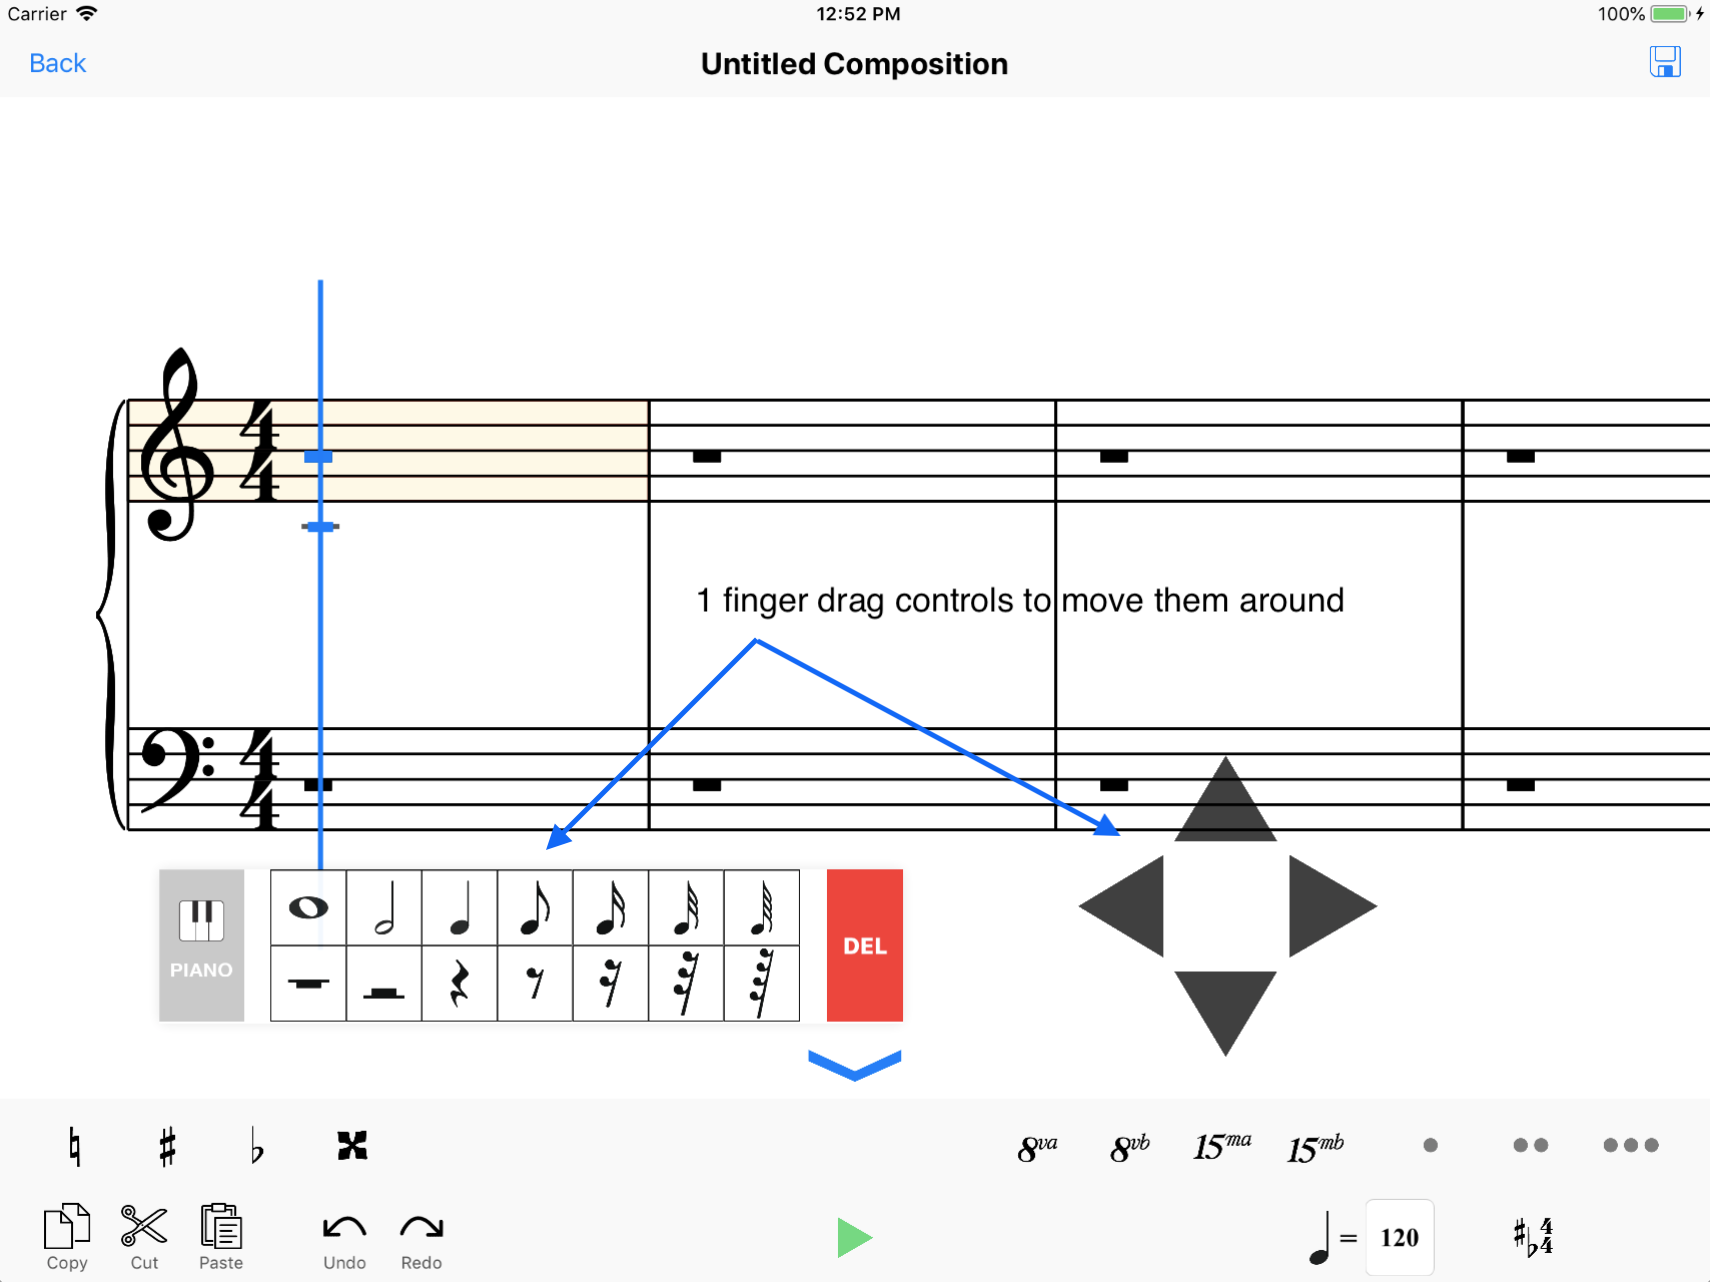
\includegraphics[scale=0.4]{Move_Controls}
    \caption{One finger drag gesture to move controls.}
    \label{fig:move-controls}
\end{figure}

\section{Renaming a Composition}
Initially, the title of a new composition is set to "Untitled Composition", and the user may edit it by tapping on the title text above in the application toolbar. 

\begin{figure}[H]
  \centering
  
\includegraphics[scale=0.7]{Renaming}
    \caption{Renaming a composition.}
    \label{fig:renaming}
\end{figure}

\section{Moving the Cursor}
The blue cursor indicates where the next note or rest will be placed, and it also indicates the selected measure and the selected note or rest. There are currently three ways on how the user may move the blue cursor in the editor. The first way is through the use of the arrow controls. Tapping on the up or down arrow keys will change the pitch of the cursor either higher or lower by a half step (Figure \ref{fig:move-arrow-up}). Tapping on the left and right arrow keys, on the other hand, will move the selection of the cursor either to the previous or next note (Figure \ref{fig:move-arrow-right}). The second way of moving the cursor is by dragging it. Upon dragging the cursor, the horizontal line will elongate which indicates that the cursor is already being dragged by the user and also for the user to easily see the current location of the cursor (Figure \ref{fig:cursor-drag}). The third way is by tapping on a location in the editor. Doing so will automatically move the cursor on the tapped location (Figure \ref{fig:cursor-tap}).

\begin{figure}[H]
  \centering
  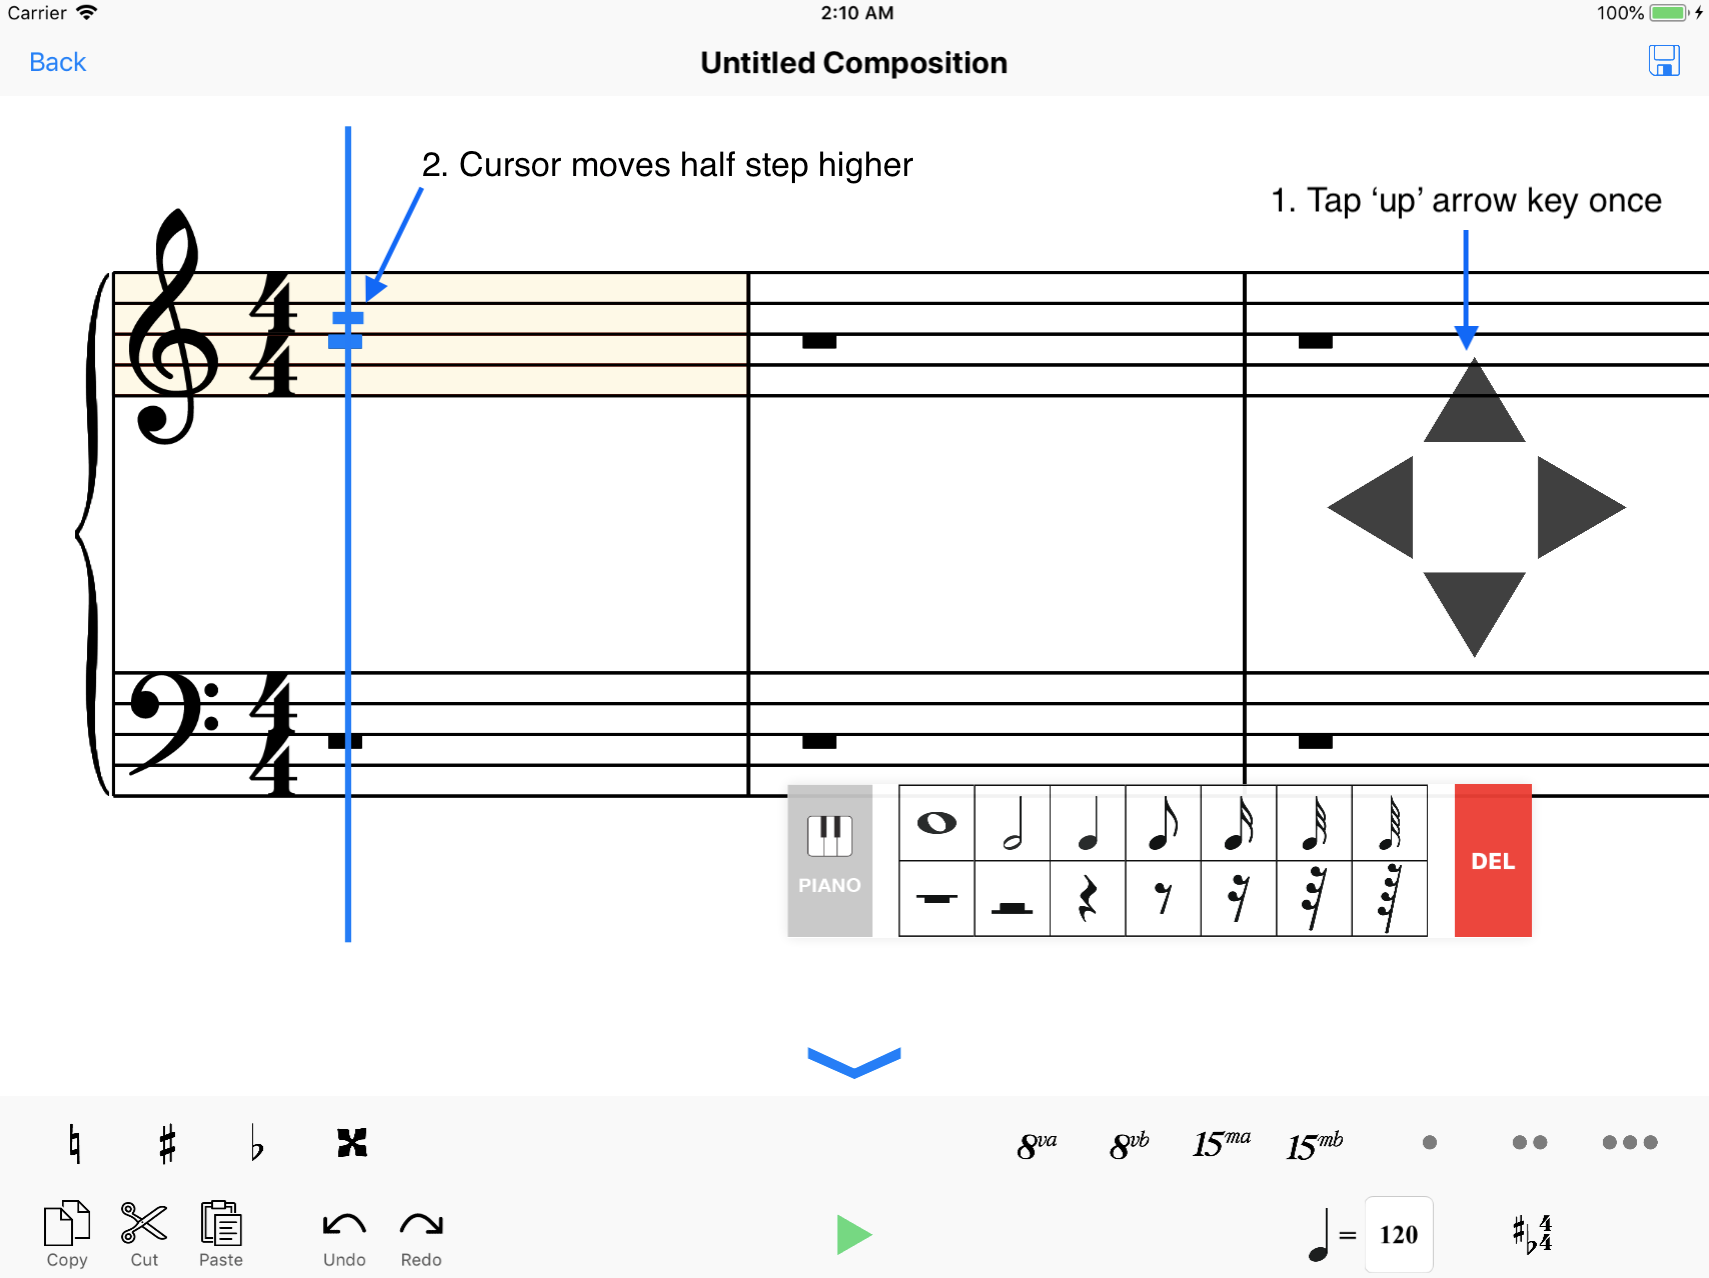
\includegraphics[scale=0.5]{Move_Arrow_Up}
    \caption{Move cursor by a half step higher.}
    \label{fig:move-arrow-up}
\end{figure}

\begin{figure}[H]
  \centering
  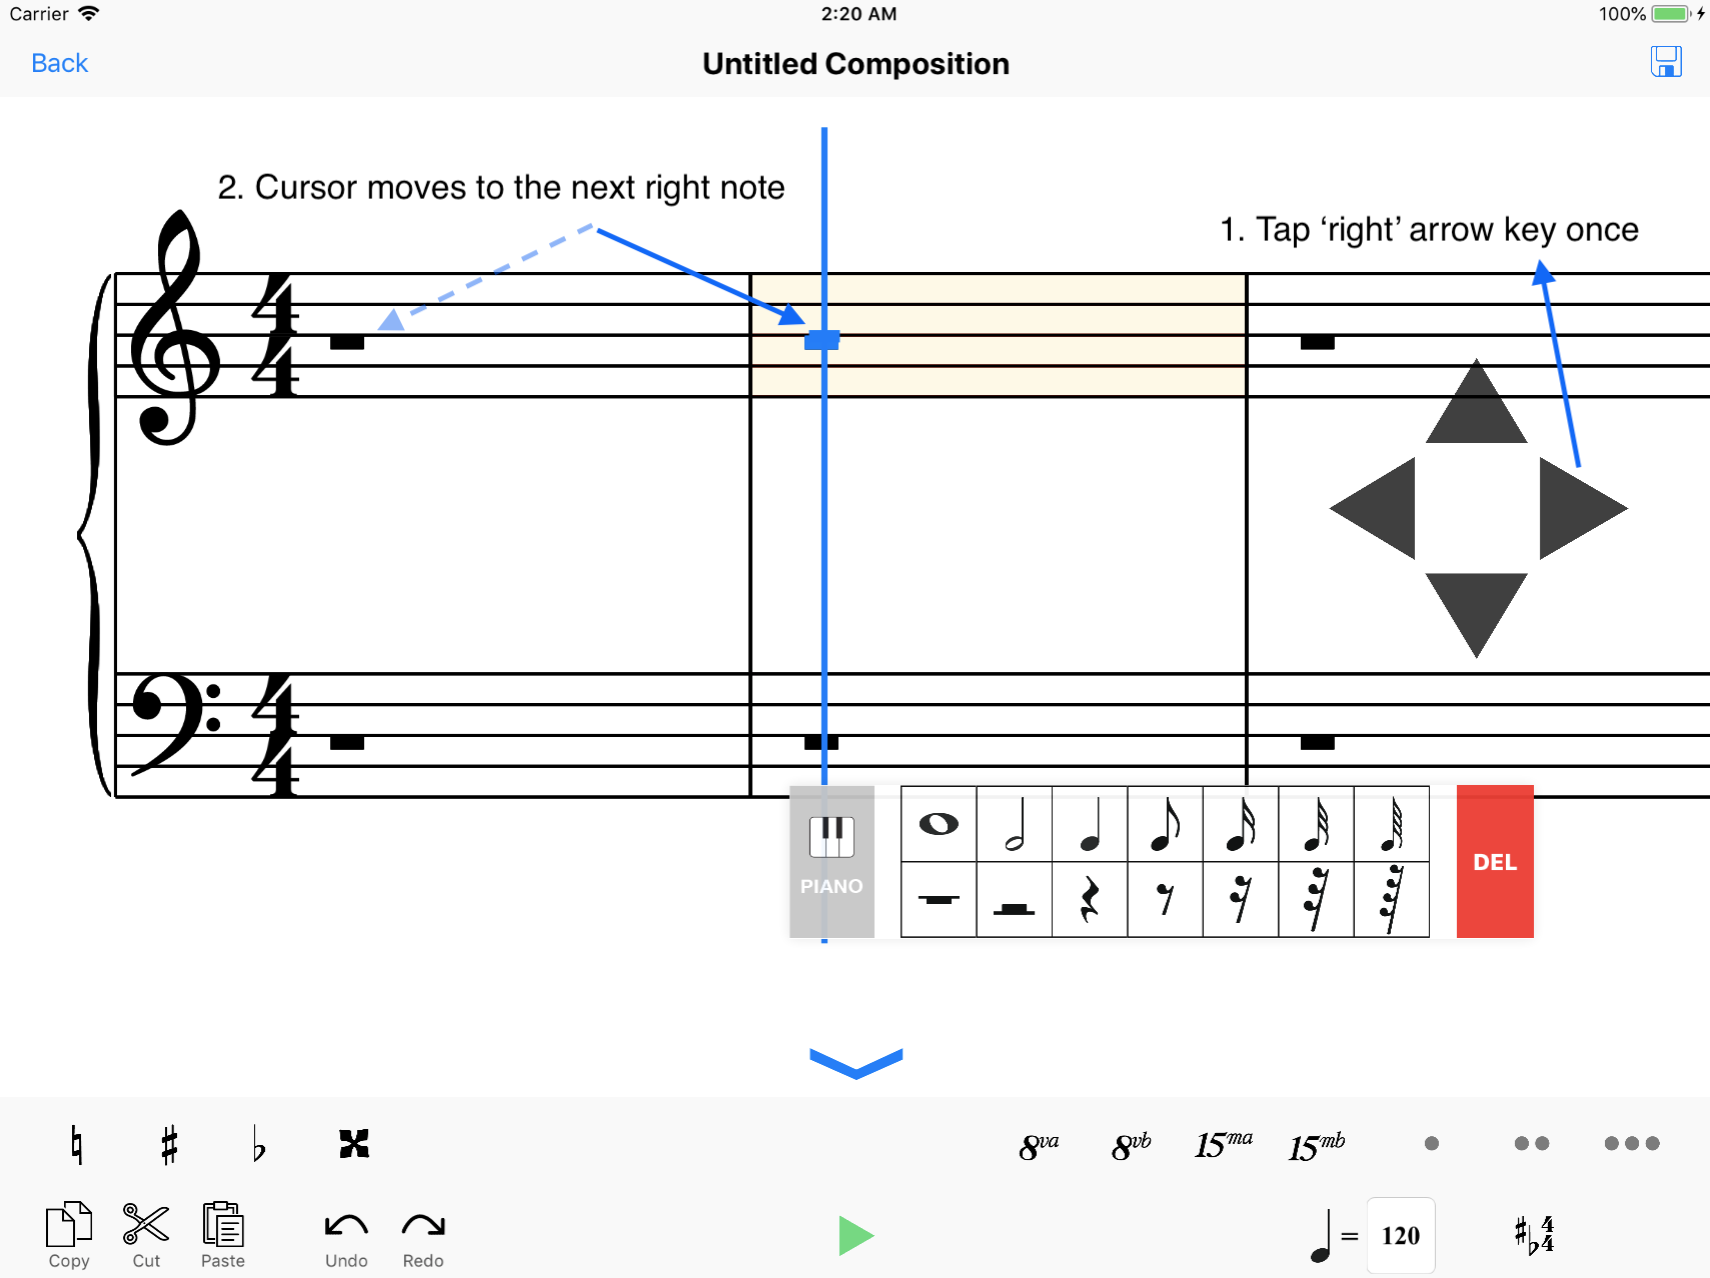
\includegraphics[scale=0.4]{Move_Arrow_Right}
    \caption{Move cursor next note to the right.}
    \label{fig:move-arrow-right}
\end{figure}

\begin{figure}[H]
  \centering
  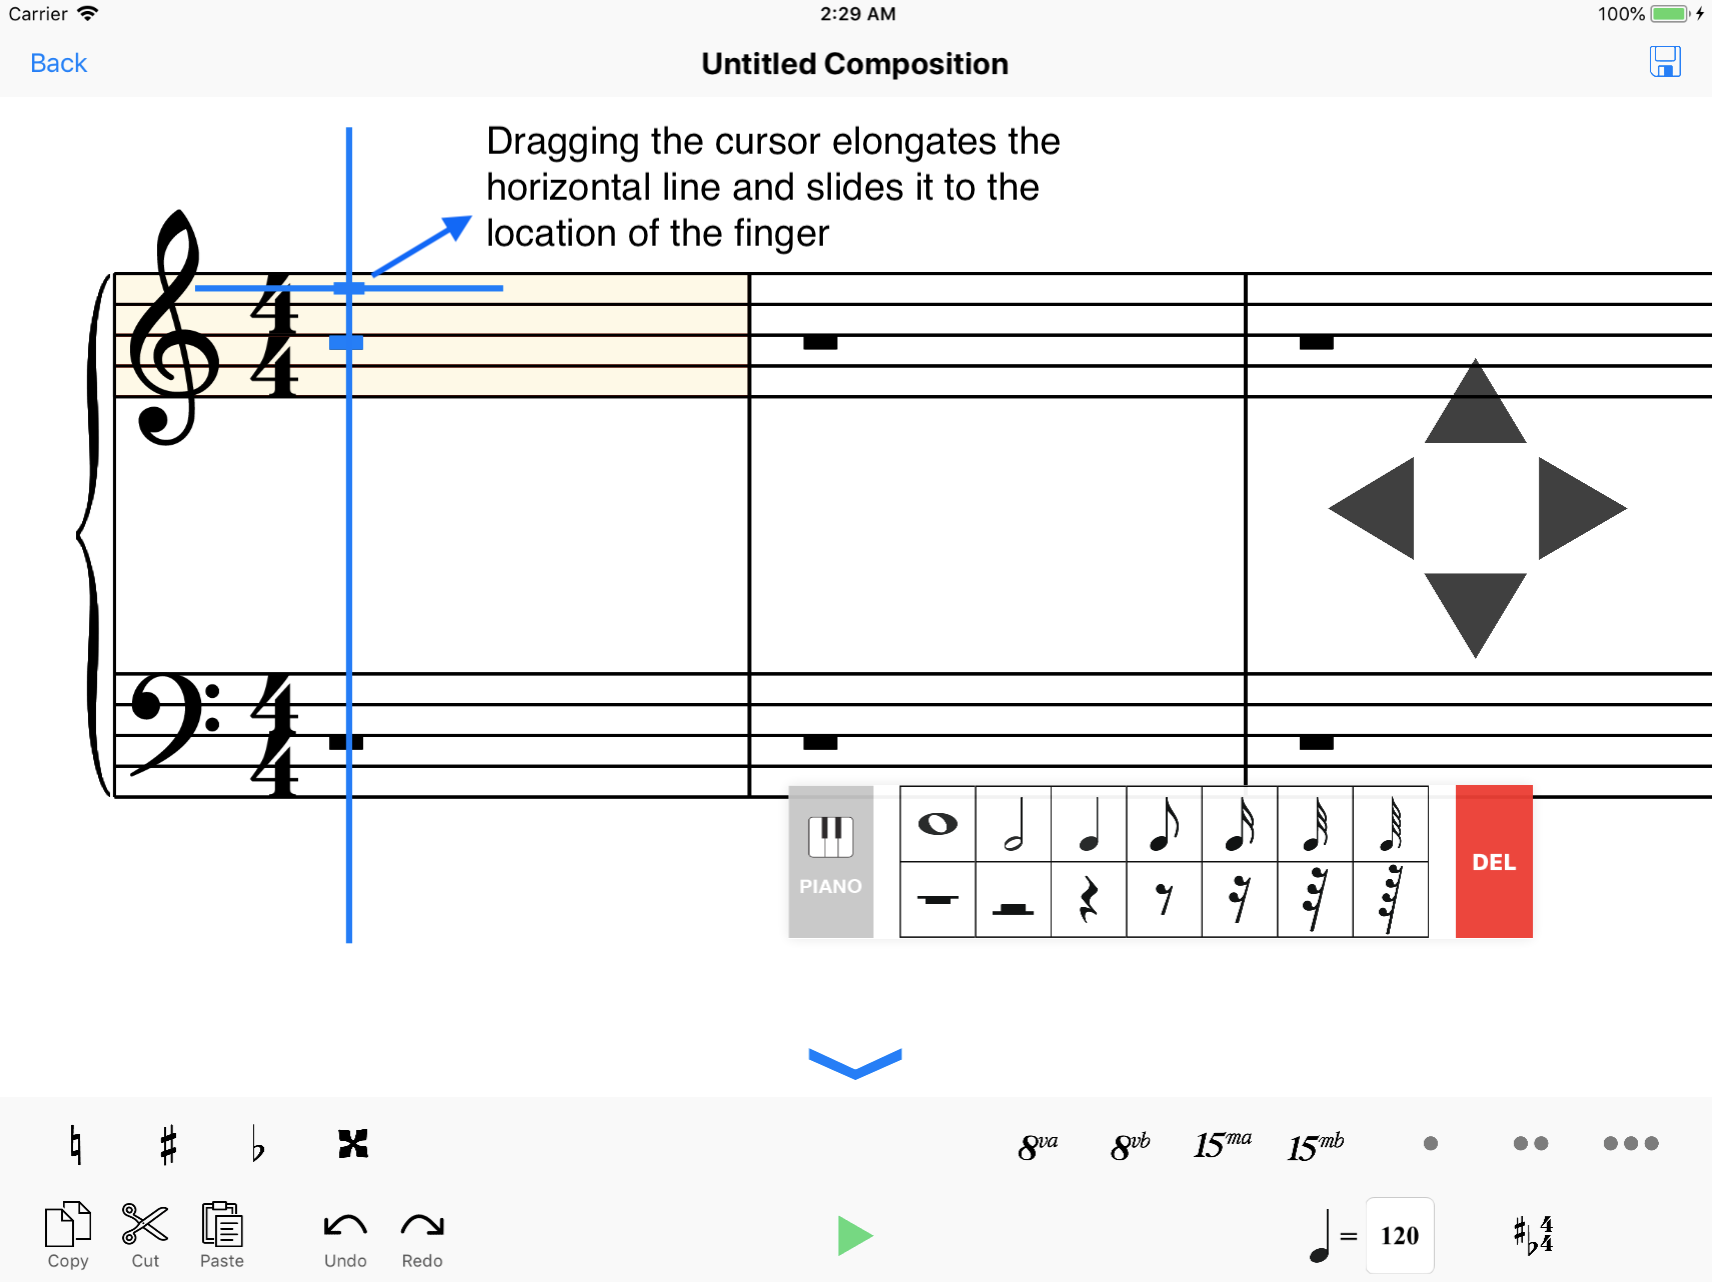
\includegraphics[scale=0.4]{Cursor_Drag}
    \caption{Dragging a cursor.}
    \label{fig:cursor-drag}
\end{figure}

\begin{figure}[H]
  \centering
  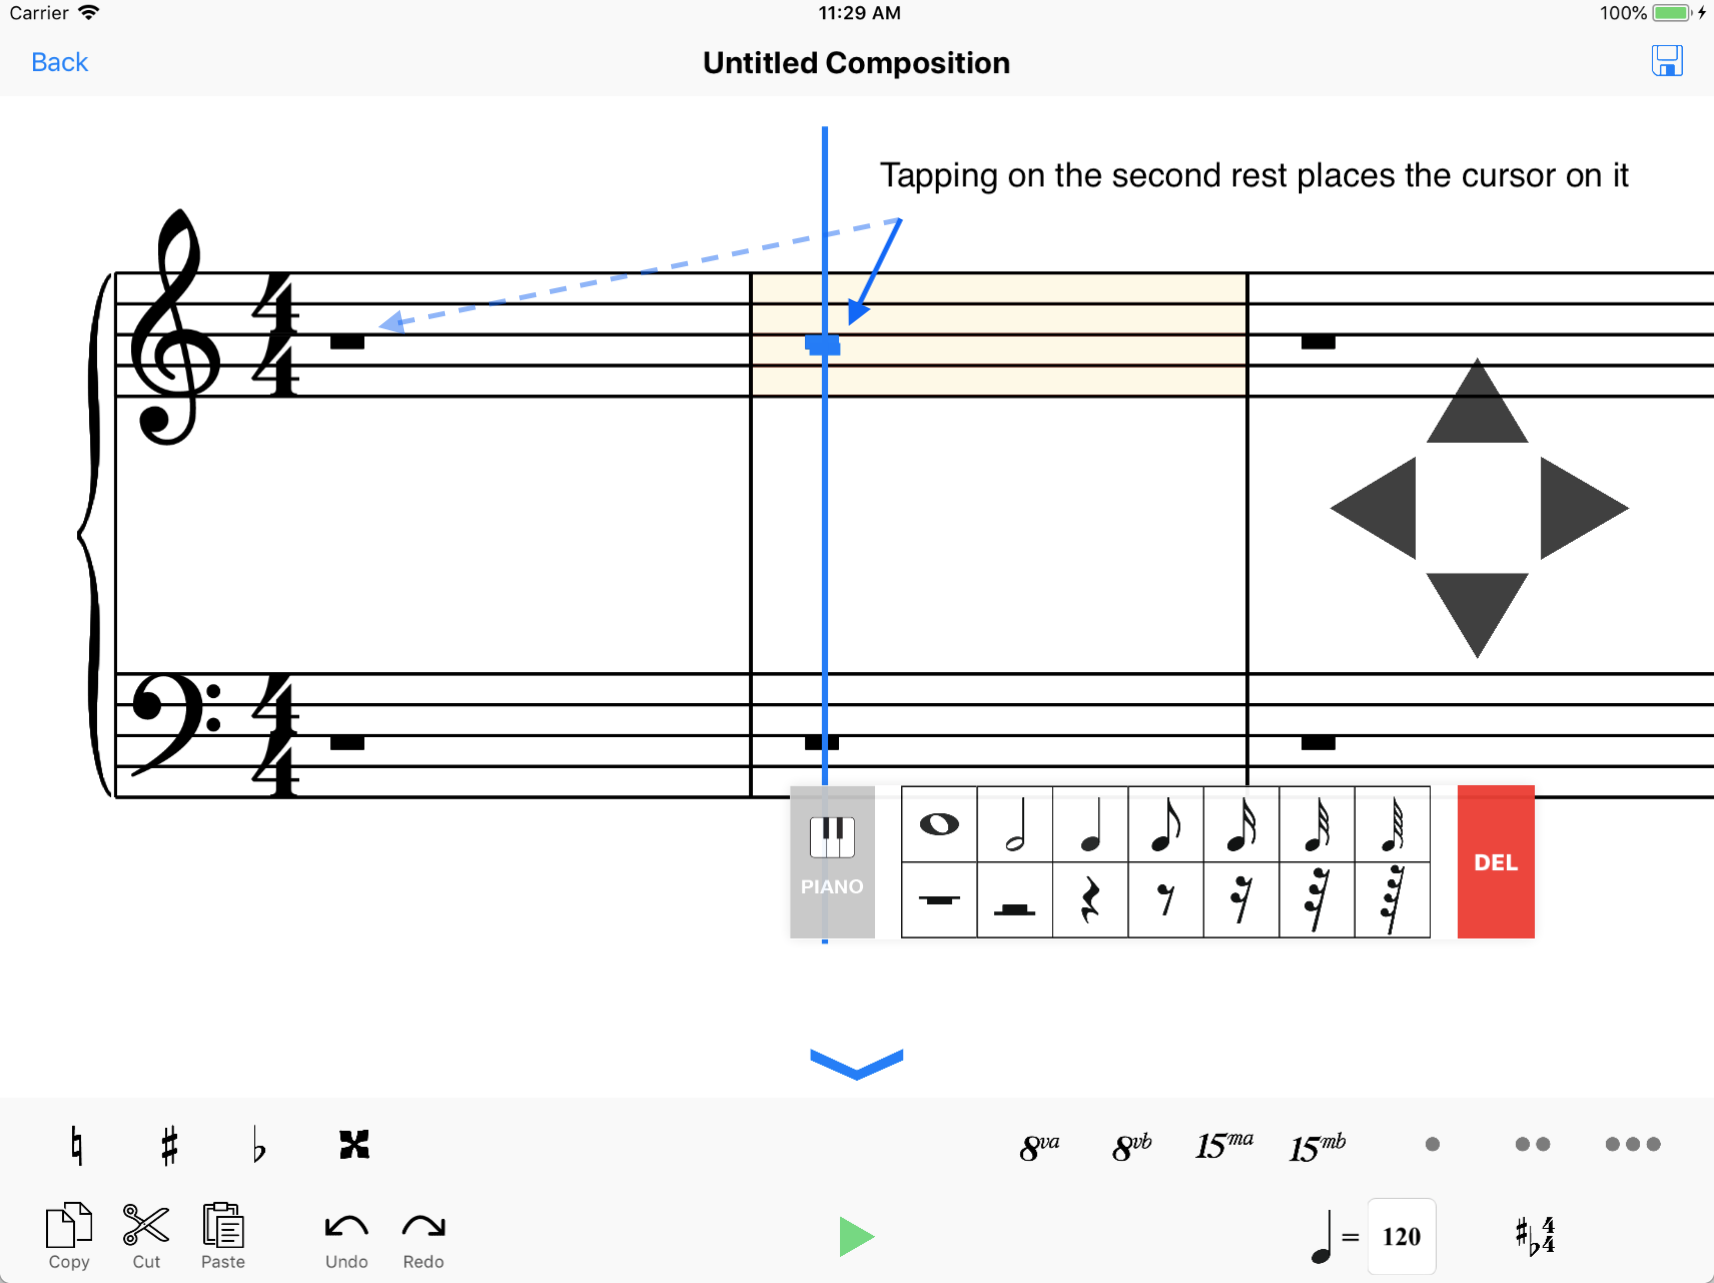
\includegraphics[scale=0.4]{Tap_Cursor}
    \caption{Tap on a location on the editor to move the cursor to it.}
    \label{fig:cursor-tap}
\end{figure}

\section{Selecting Notes}
A blue highlight on a note or rest indicates that it is currently selected. When a cursor is in the same x-axis with a single note or rest, that note or rest is selected and the user may perform different actions on it such as transpose, edit, or delete (Figure \ref{fig:selected-rest}).

\begin{figure}[H]
  \centering
  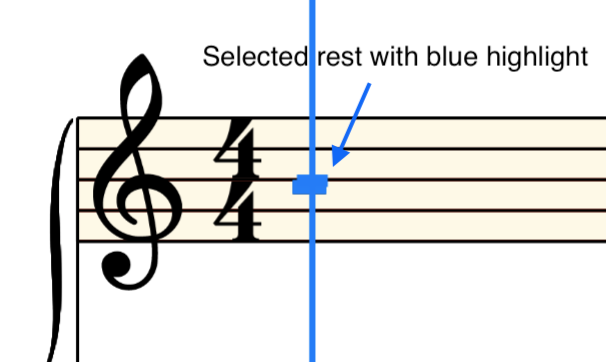
\includegraphics[scale=0.8]{Selected_Rest}
    \caption{Selected rest with blue highlight.}
    \label{fig:selected-rest}
\end{figure}

For selecting multiples notes or rests, the user must do a 1 finger drag gesture in a diagonal direction to bring out the rectangle selector which indicates the area it is currently selecting (Figure \ref{fig:drag-selection}).

\begin{figure}[H]
  \centering
  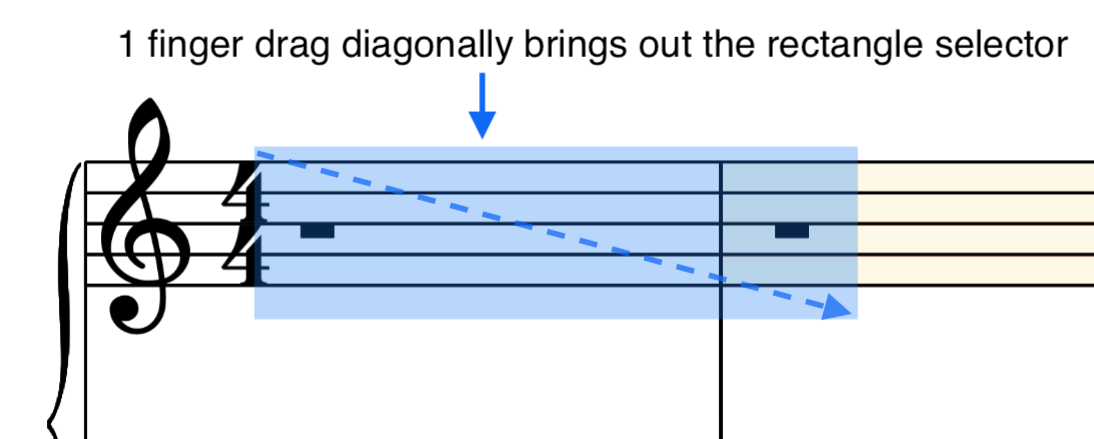
\includegraphics[scale=0.7]{Drag_Selection}
    \caption{1 finger drag diagonally brings out the rectangle selector.}
    \label{fig:drag-selection}
\end{figure}

When the user releases the drag gesture, the rectangle will select the notes it encompassed. Additionally, when more than one rest or note is selected using the drag gesture, it will bring out the transform view which allows the user to transpose, retrograde-inverse, and place a tie or a slur on the selected notes or rests if the rules apply. In the case of Figure \ref{fig:multiple-selected}, the retrograde-inverse and tie or slur buttons are disabled.

\begin{figure}[H]
  \centering
  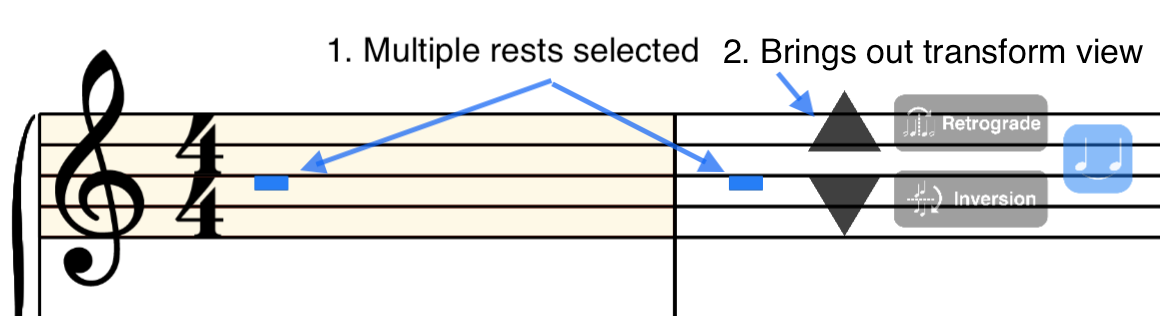
\includegraphics[scale=0.7]{Multiple_Selected}
    \caption{Multiple rests selected with blue highlight and brings out transform view.}
    \label{fig:multiple-selected}
\end{figure}

\section{Adding a Note or Rest}
Initially, upon creating or opening a composition, the blue cursor automatically selects the first note or rest in the first measure of the composition (Figure \ref{fig:editor}). To add a note or a rest, simply tap on a note type in the notation controls in the editor screen and the note will automatically be added on the location of the blue cursor (Figure \ref{fig:add-note-rest}).

\begin{figure}[H]
  \centering
  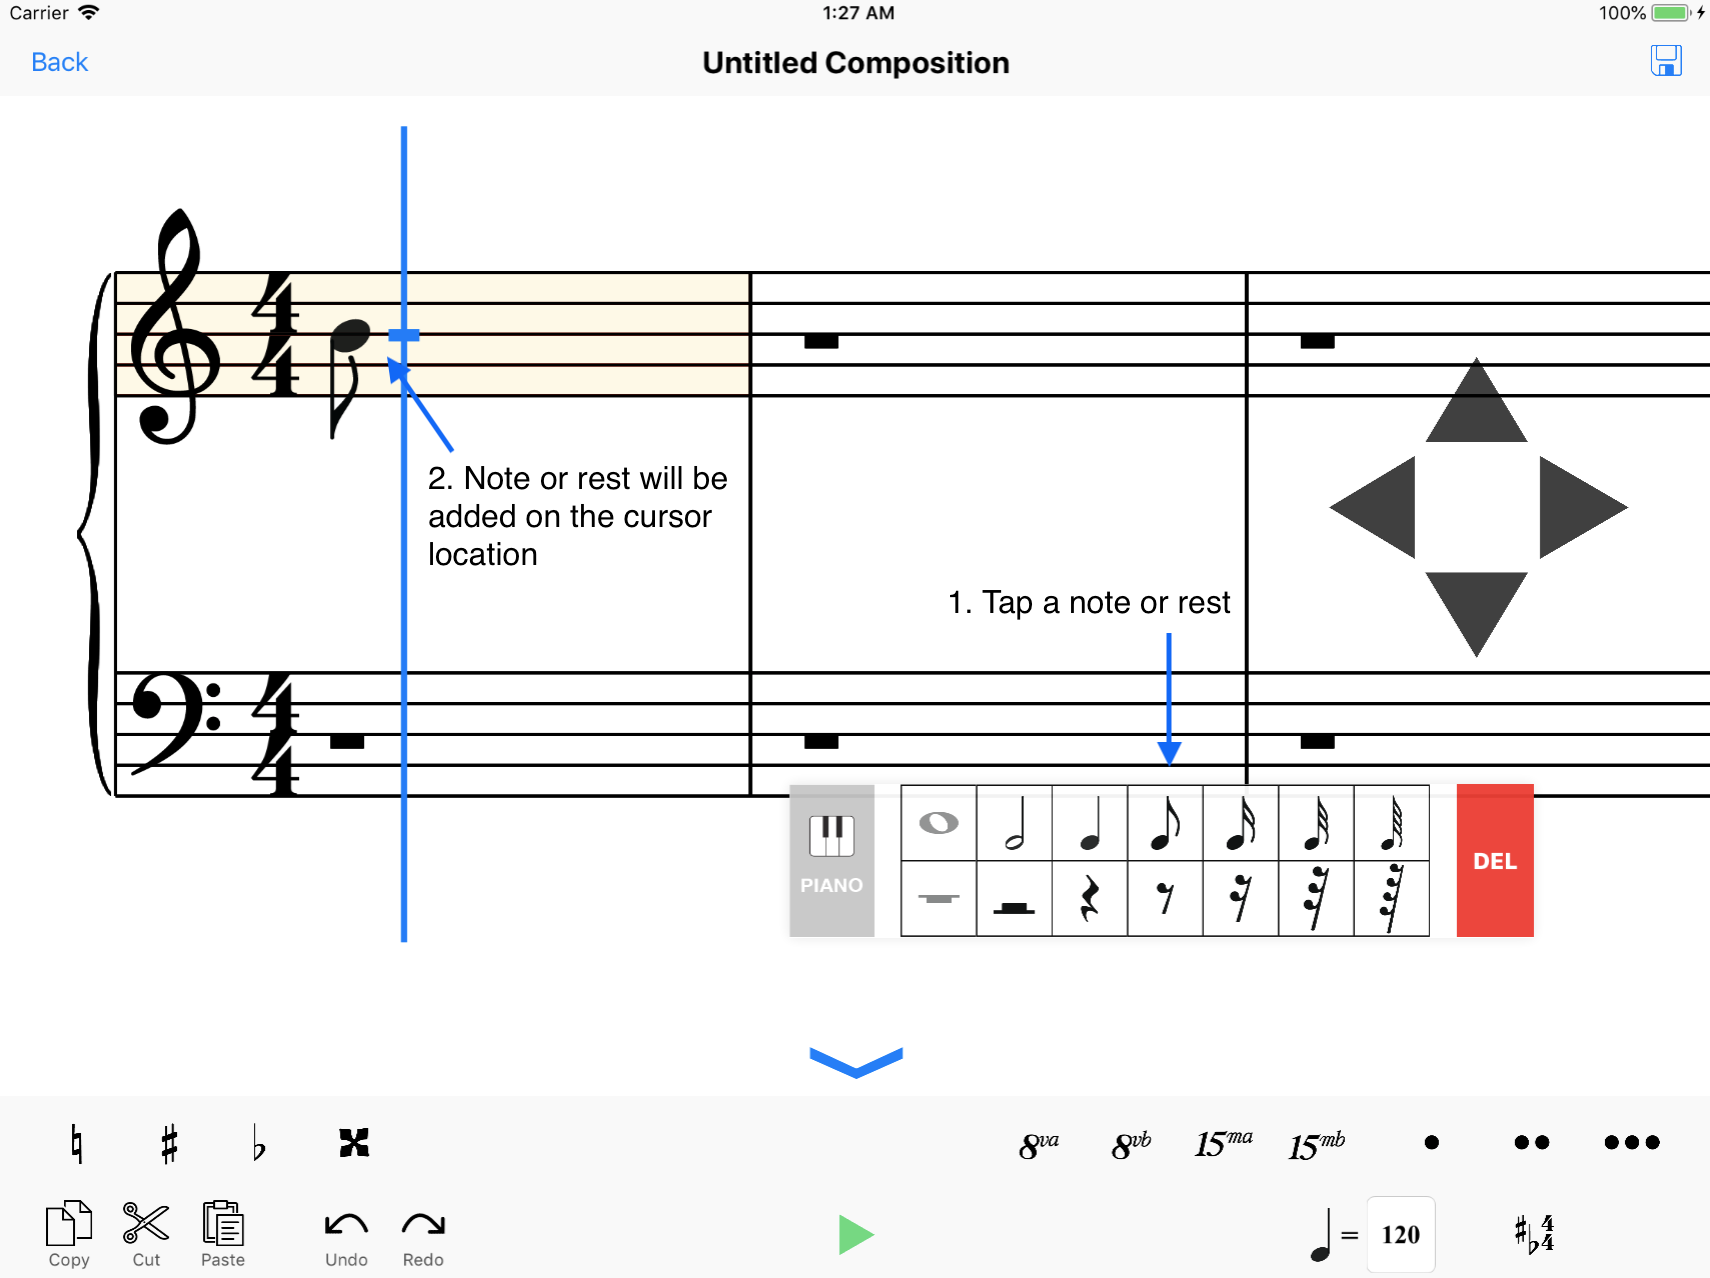
\includegraphics[scale=0.5]{Add_Note_or_Rest}
    \caption{Adding a note or rest.}
    \label{fig:add-note-rest}
\end{figure}

\section{Adding Polyphony}
To add polyphony, the user must place the cursor above or below an existing note and add a note using the same note type with the existing note.

\begin{figure}[H]
  \centering
  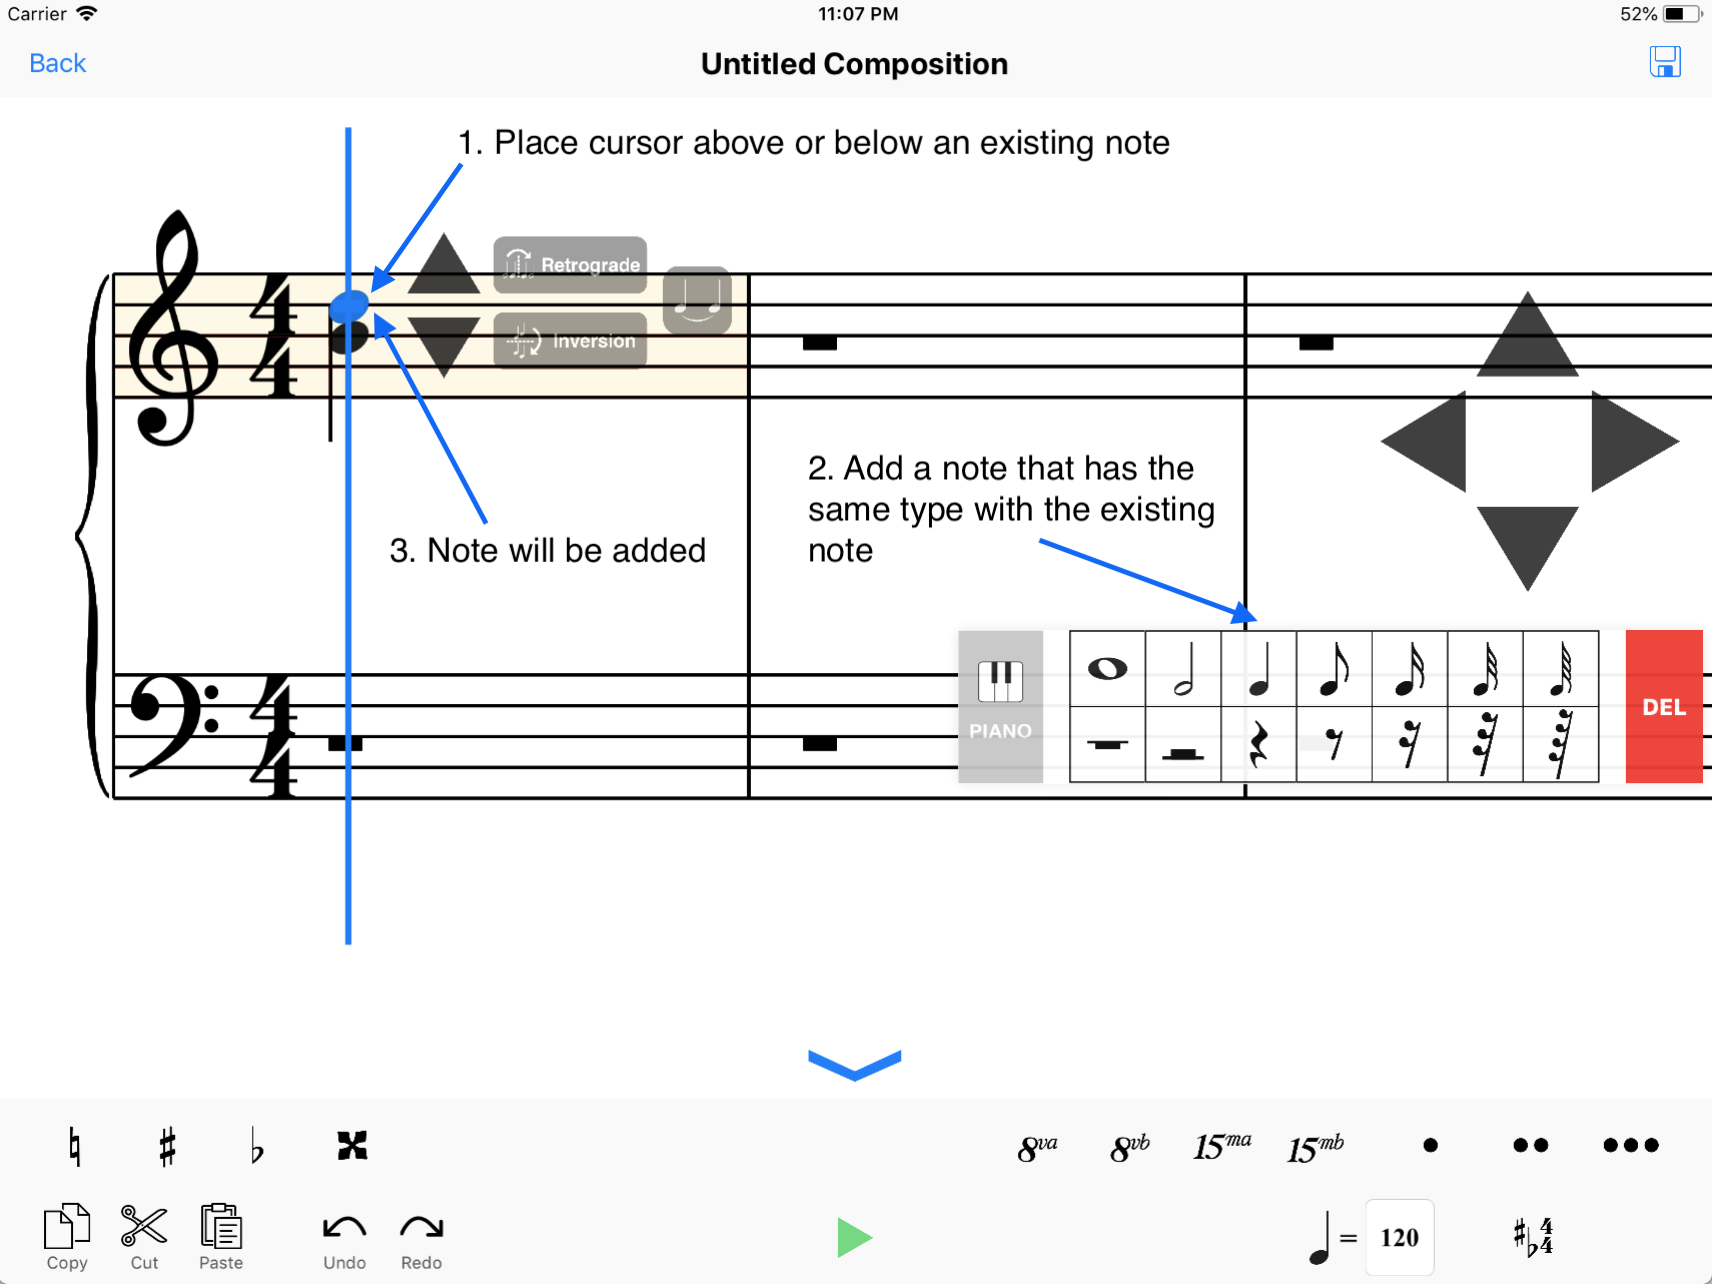
\includegraphics[scale=0.5]{Polyphonic}
    \caption{Adding polyphony.}
    \label{fig:polyphony}
\end{figure}

\section{Editing Notes}
To edit a note or a group of notes, the user must select the notes that needs editing and tap on the new note type in the notation controls to change the selected notes (Figure \ref{fig:edit-note}).

\begin{figure}[H]
  \centering
  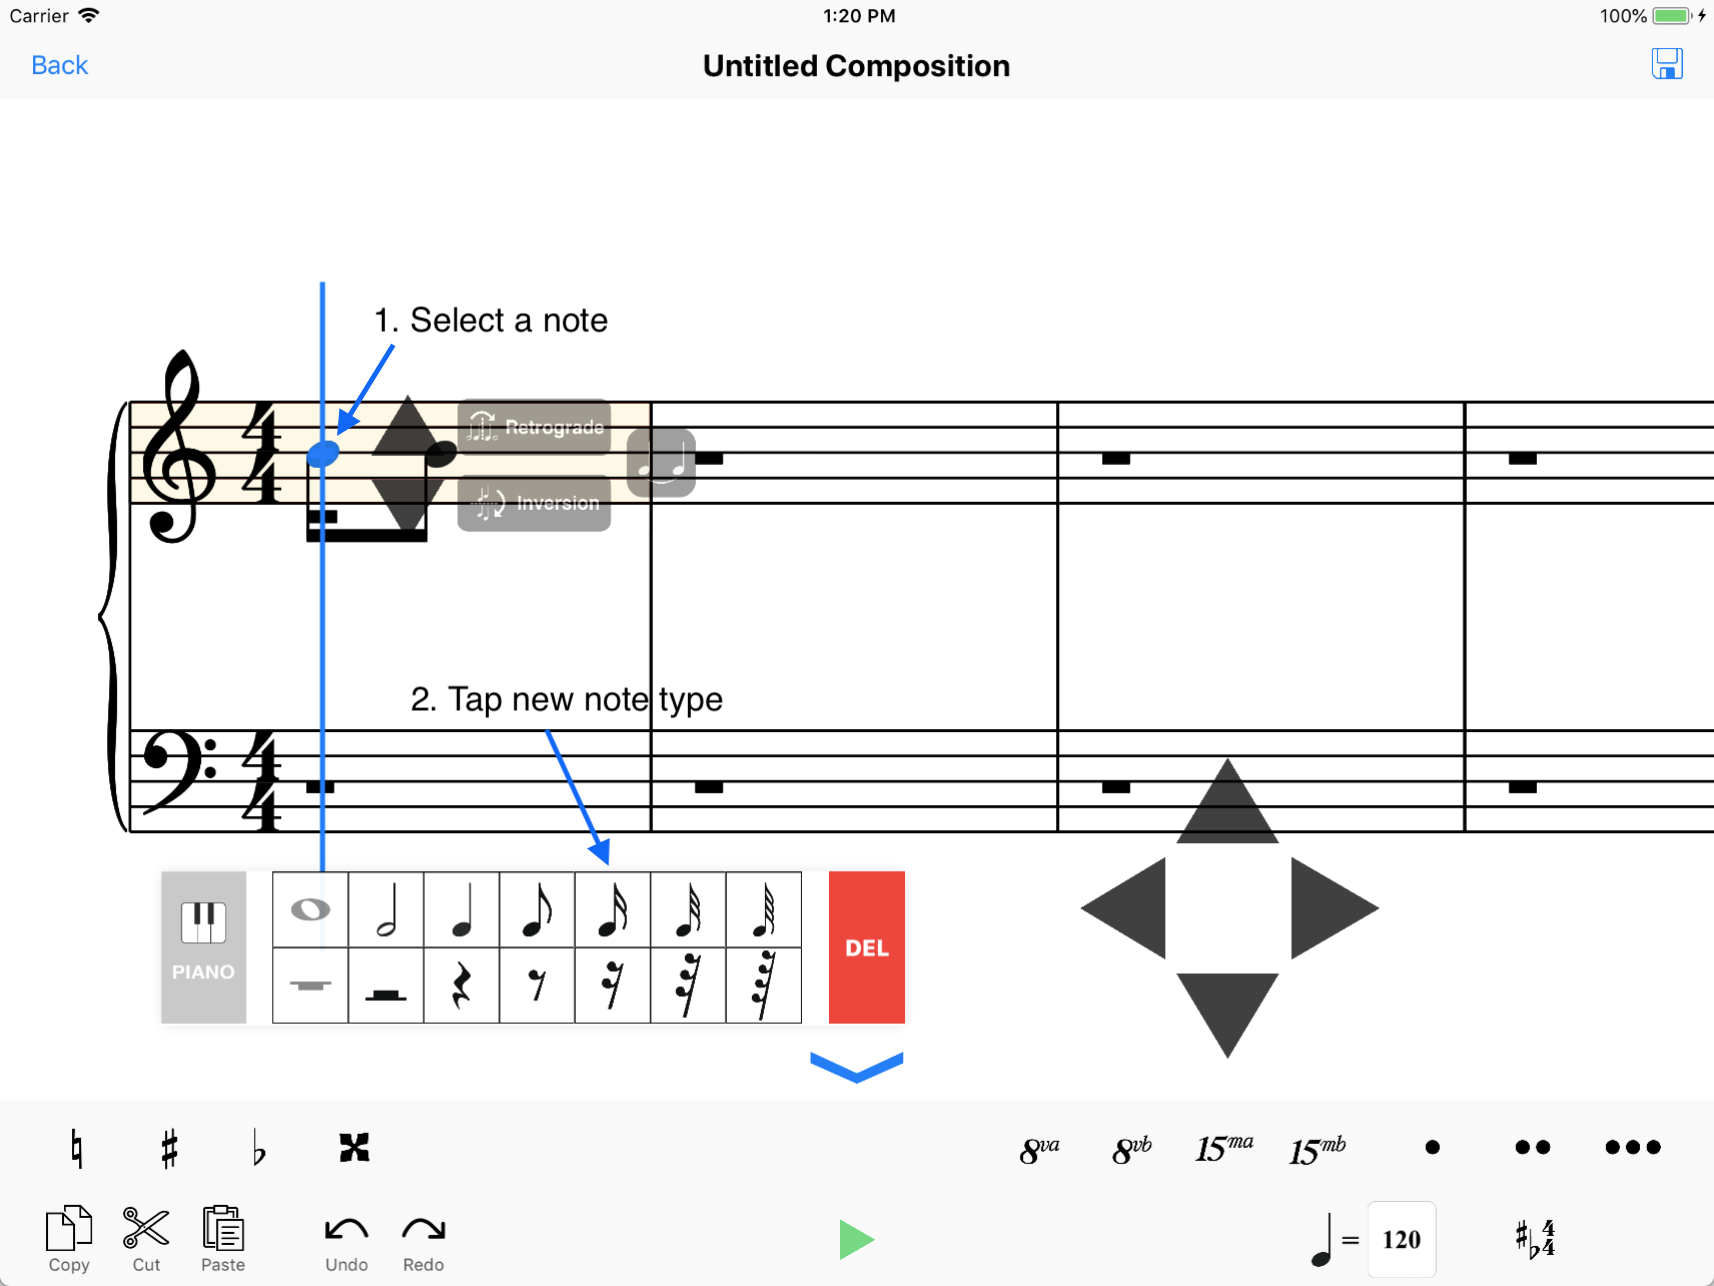
\includegraphics[scale=0.5]{Edit_Note}
    \caption{Editing notes.}
    \label{fig:edit-note}
\end{figure}

\section{Deleting Notes}
To delete a note or a group of notes, the user must select the notes that needs to be deleted and tap on the delete button in the notation controls to delete the selected notes (Figure \ref{fig:delete-notes}).

\begin{figure}[H]
  \centering
  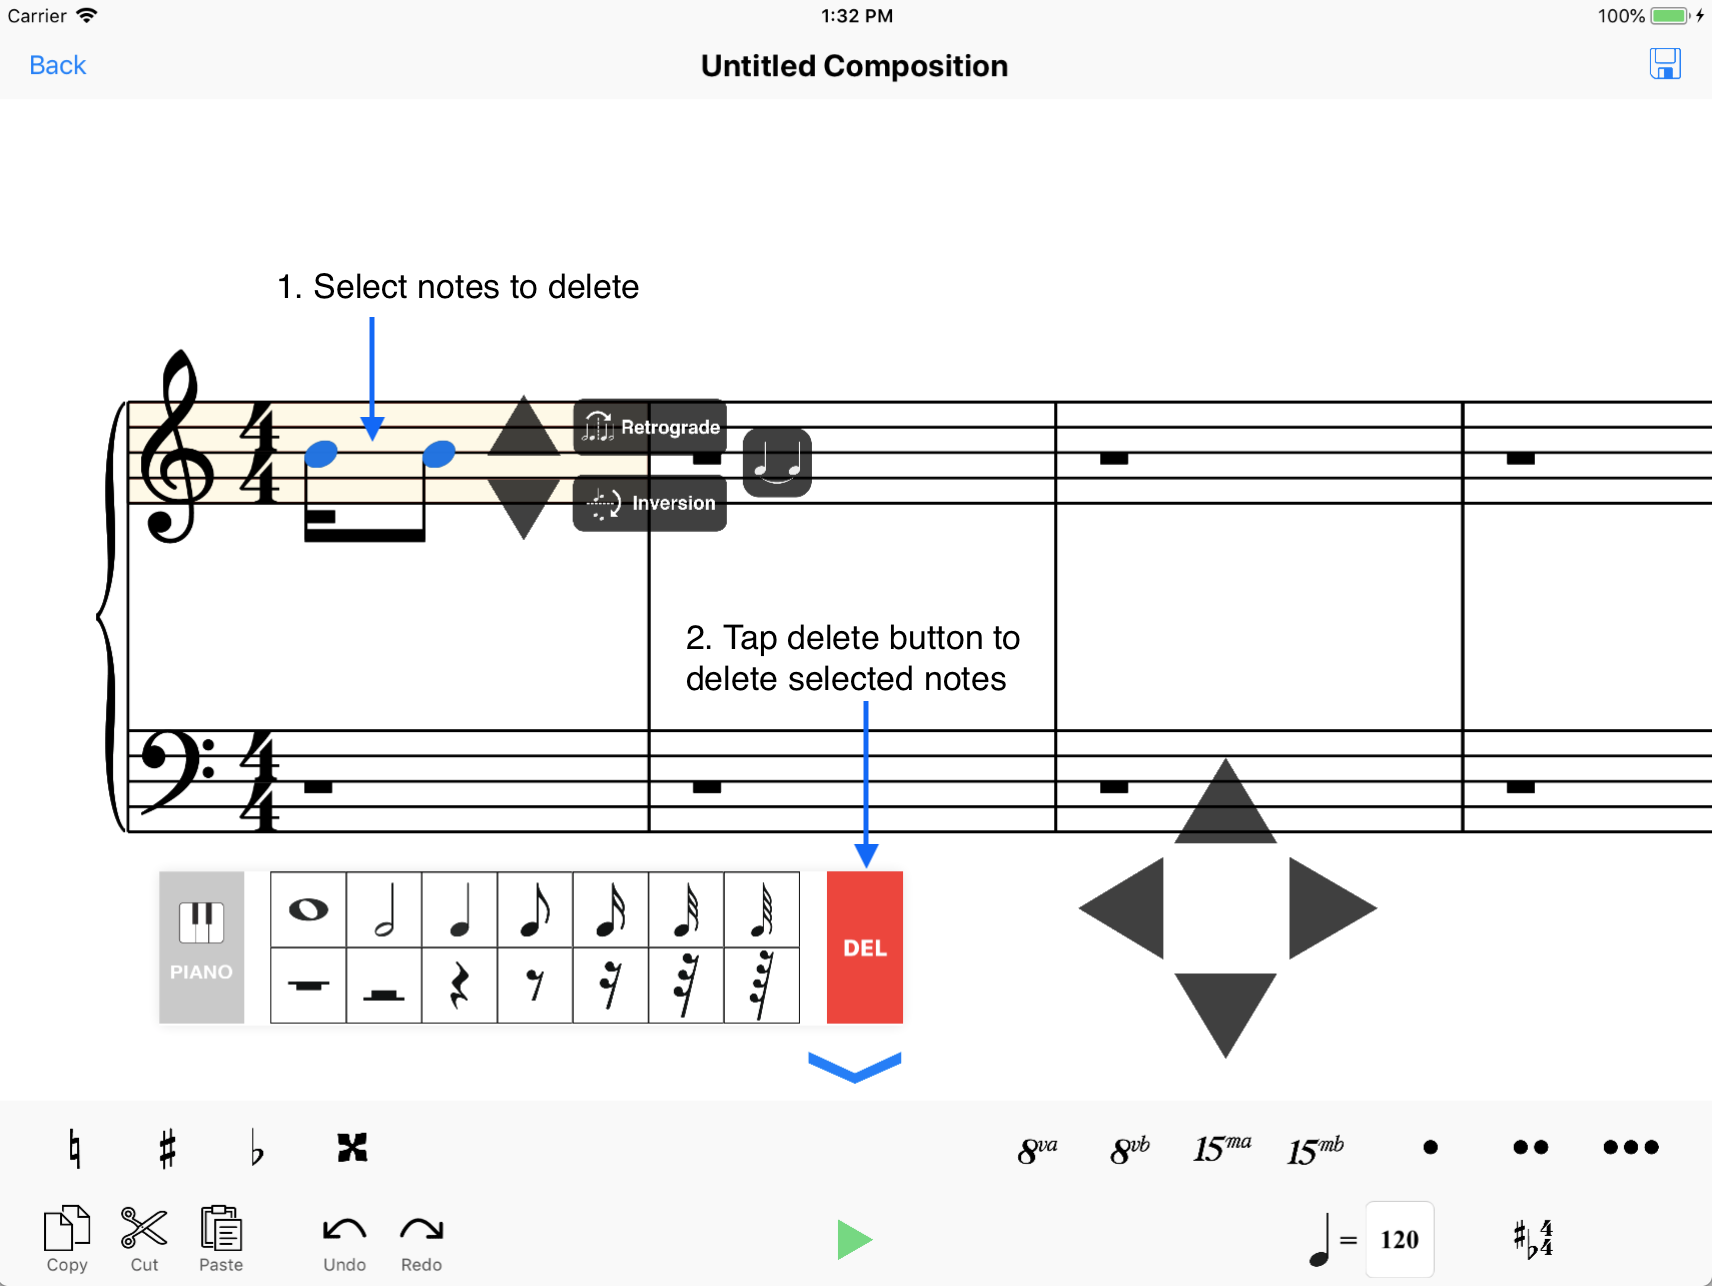
\includegraphics[scale=0.5]{Delete_Notes}
    \caption{Deleting notes.}
    \label{fig:delete-notes}
\end{figure}

\section{Transposing a Note or a Group of Notes}
To transpose a note or a group of notes, the user must select the notes that needs to be transposed to show the transpose buttons. Upon selecting the notes, the user may tap on the up or down arrow keys beside the selected notes to transpose them half step higher or lower, respectively (Figure \ref{fig:transposing}).

\begin{figure}[H]
  \centering
  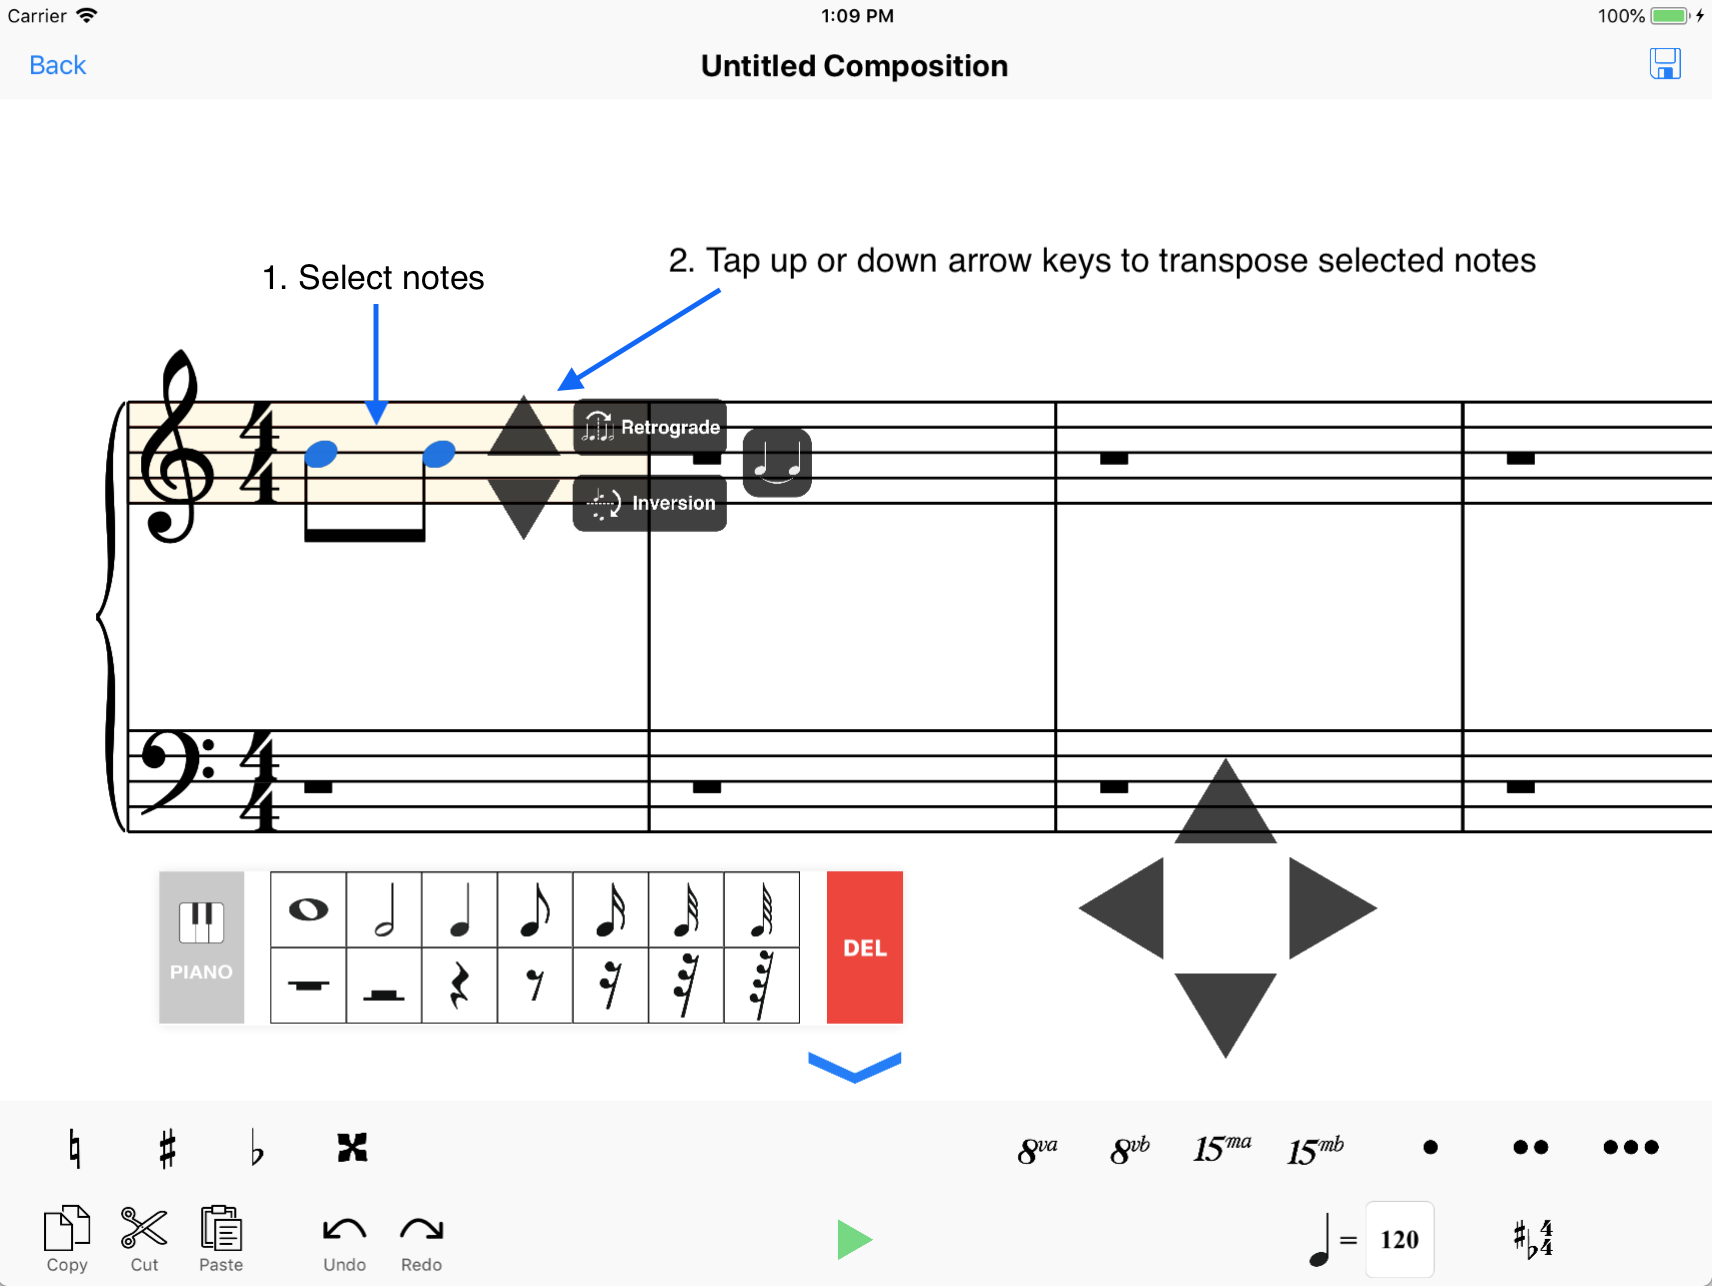
\includegraphics[scale=0.5]{Transposing}
    \caption{Transposing notes.}
    \label{fig:transposing}
\end{figure}

\section{Retrograde - Inversion}
Retrograde - inversion can be performed only if there are more than one note selected. The transform view beside the selected notes will appear upon selecting notes and the retrograde and inverse buttons will be enabled allowing the user to tap either of them (Figure \ref{fig:r-i}).

\begin{figure}[H]
  \centering
  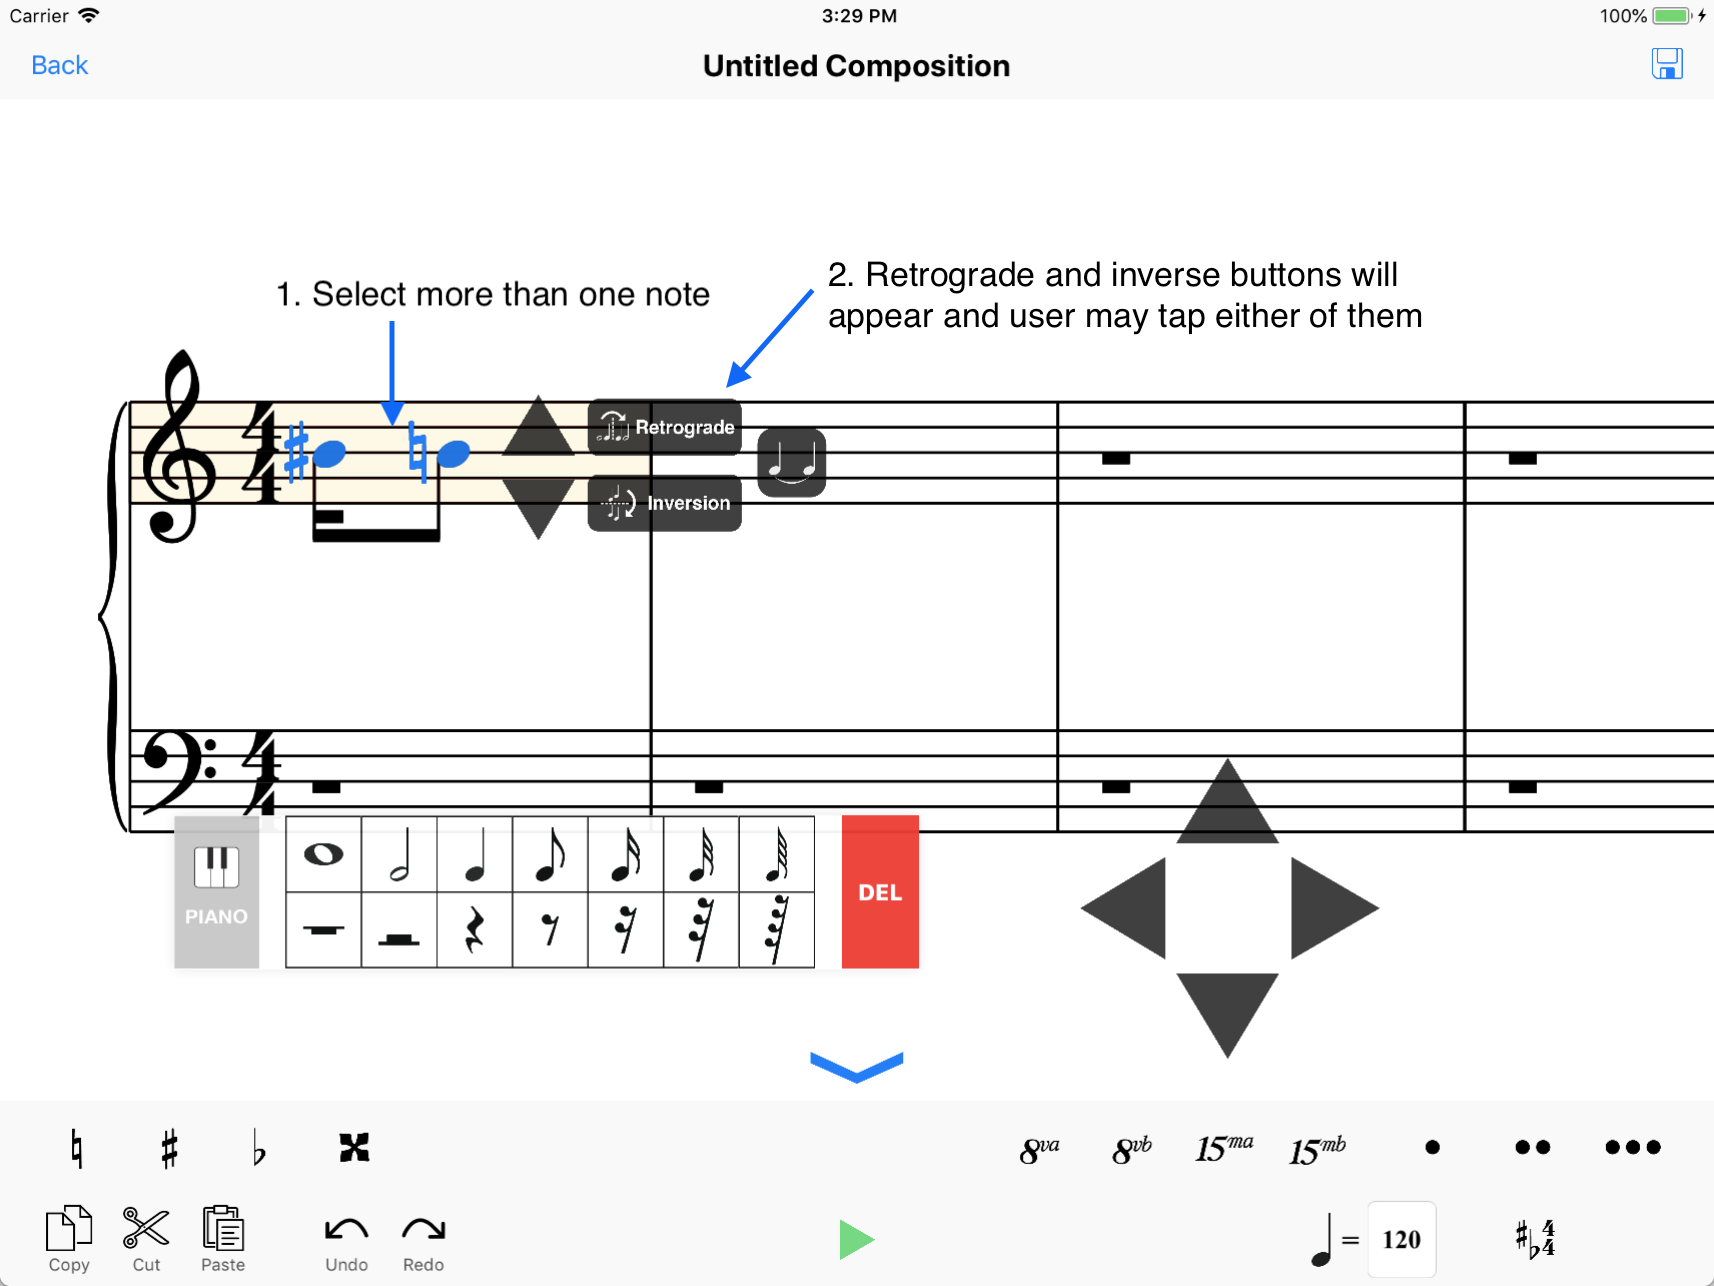
\includegraphics[scale=0.5]{Retrograde_Inverse}
    \caption{Performing a retrograde or inversion on a group of notes.}
    \label{fig:r-i}
\end{figure}

\section{Adding Ties or Slurs}
Ties or slurs could be added by selecting more than one note. The transform view beside the selected notes will appear and the tie or slur button will be enabled allowing the user to add a tie or slur on the selected notes. A tie will will be added if the selected notes are all the same pitch, on the other hand, a slur will be added if at least one of the selected notes has a different pitch. Additionally, if a user transposes a note that has a tie or a slur, it automatically changes the type depending whether the connection of all the notes have the same pitch or not (Figure \ref{fig:ties-slur}).

\begin{figure}[H]
  \centering
  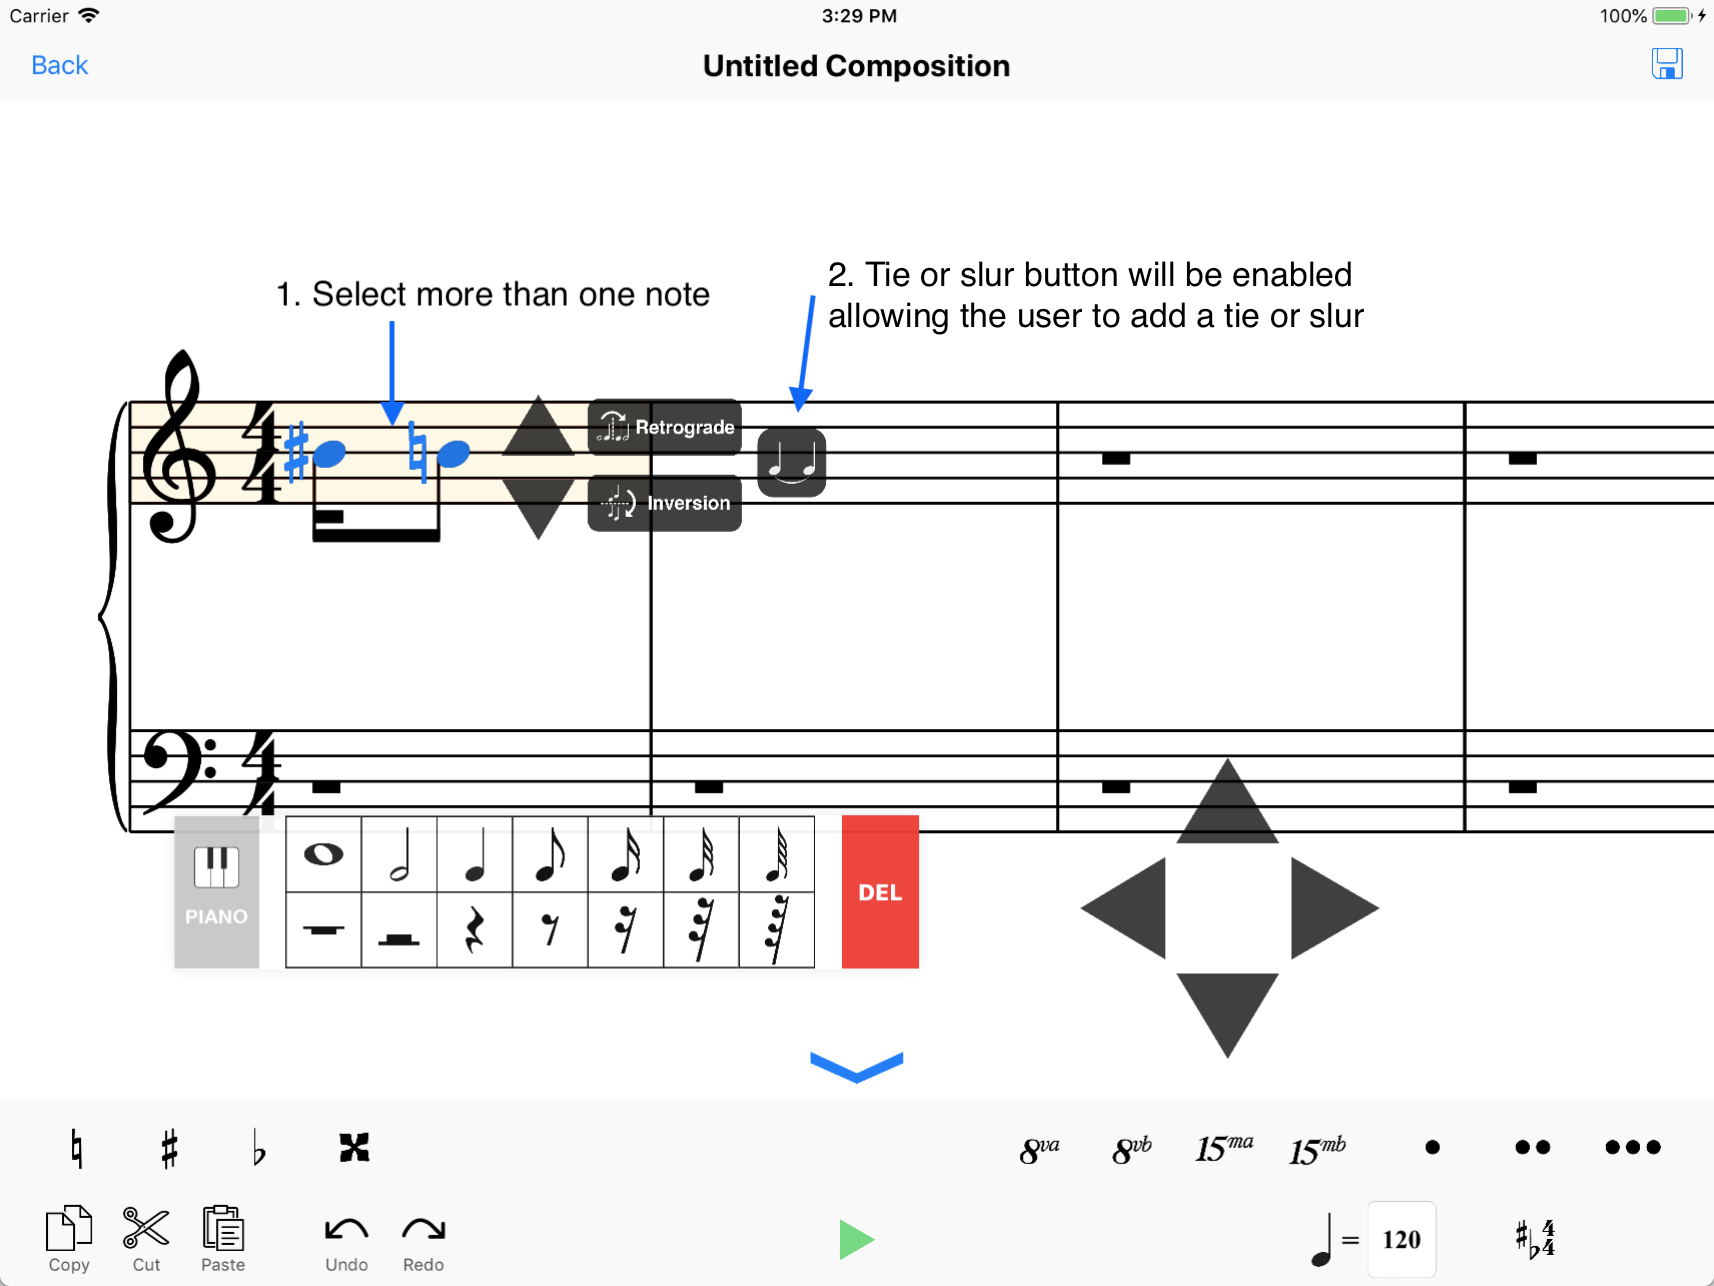
\includegraphics[scale=0.5]{Tie_Slur}
    \caption{Adding ties or slurs.}
    \label{fig:ties-slur}
\end{figure}

\section{Adding and Removing Note Accidentals, Ottava, and Dots}
The accidental buttons are located in the bottom menu of the editor. The behavior of adding and removing accidentals are similar on how the toggling of font types in word processors work. To explain further, an example would be two selected notes that initially do not have any accidentals. After tapping an accidental from the bottom menu with the two notes selected, it would change the type of accidental of all the notes selected. Selected notes with the same accidentals would highlight the accidental button with blue in the bottom menu to show that it could be toggled or tapped again to remove the accidentals in all the notes that are selected (Figure \ref{fig:add-accidental-notes}). In this example, the sharp icon is only added on the first note because the selected notes have the same pitch and the same accidental, but both notes really have a sharp accidental. This is so because of the rules of music notation.

\begin{figure}[H]
  \centering
  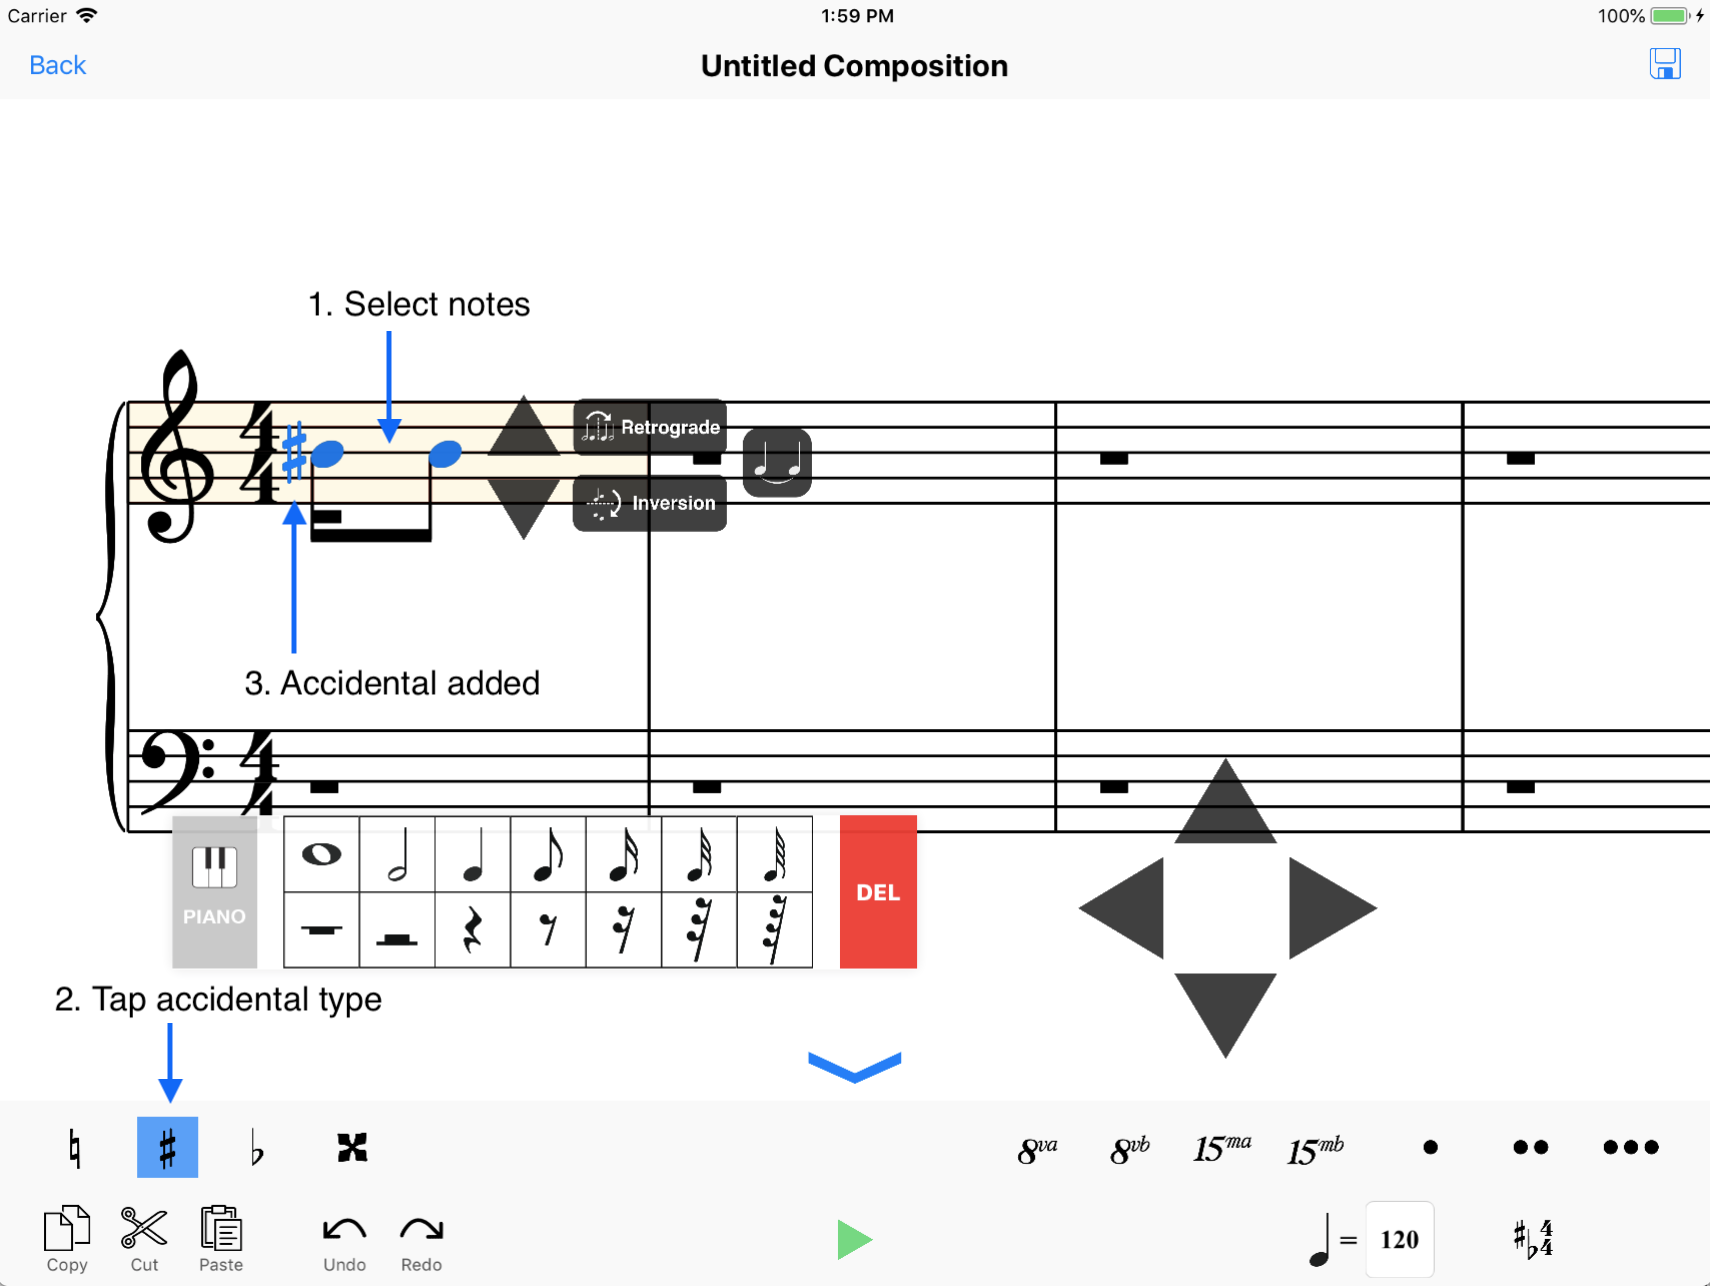
\includegraphics[scale=0.5]{Add_Accidental_Notes}
    \caption{Adding accidental on multiple notes.}
    \label{fig:add-accidental-notes}
\end{figure}

Another case would be when a note has a sharp and another note does not have an accidental. When both notes are selected, and the user taps on any accidental, it will change all the selected notes to the tapped accidental (Figure \ref{fig:change-accidental-notes}).

\begin{figure}[H]
  \centering
  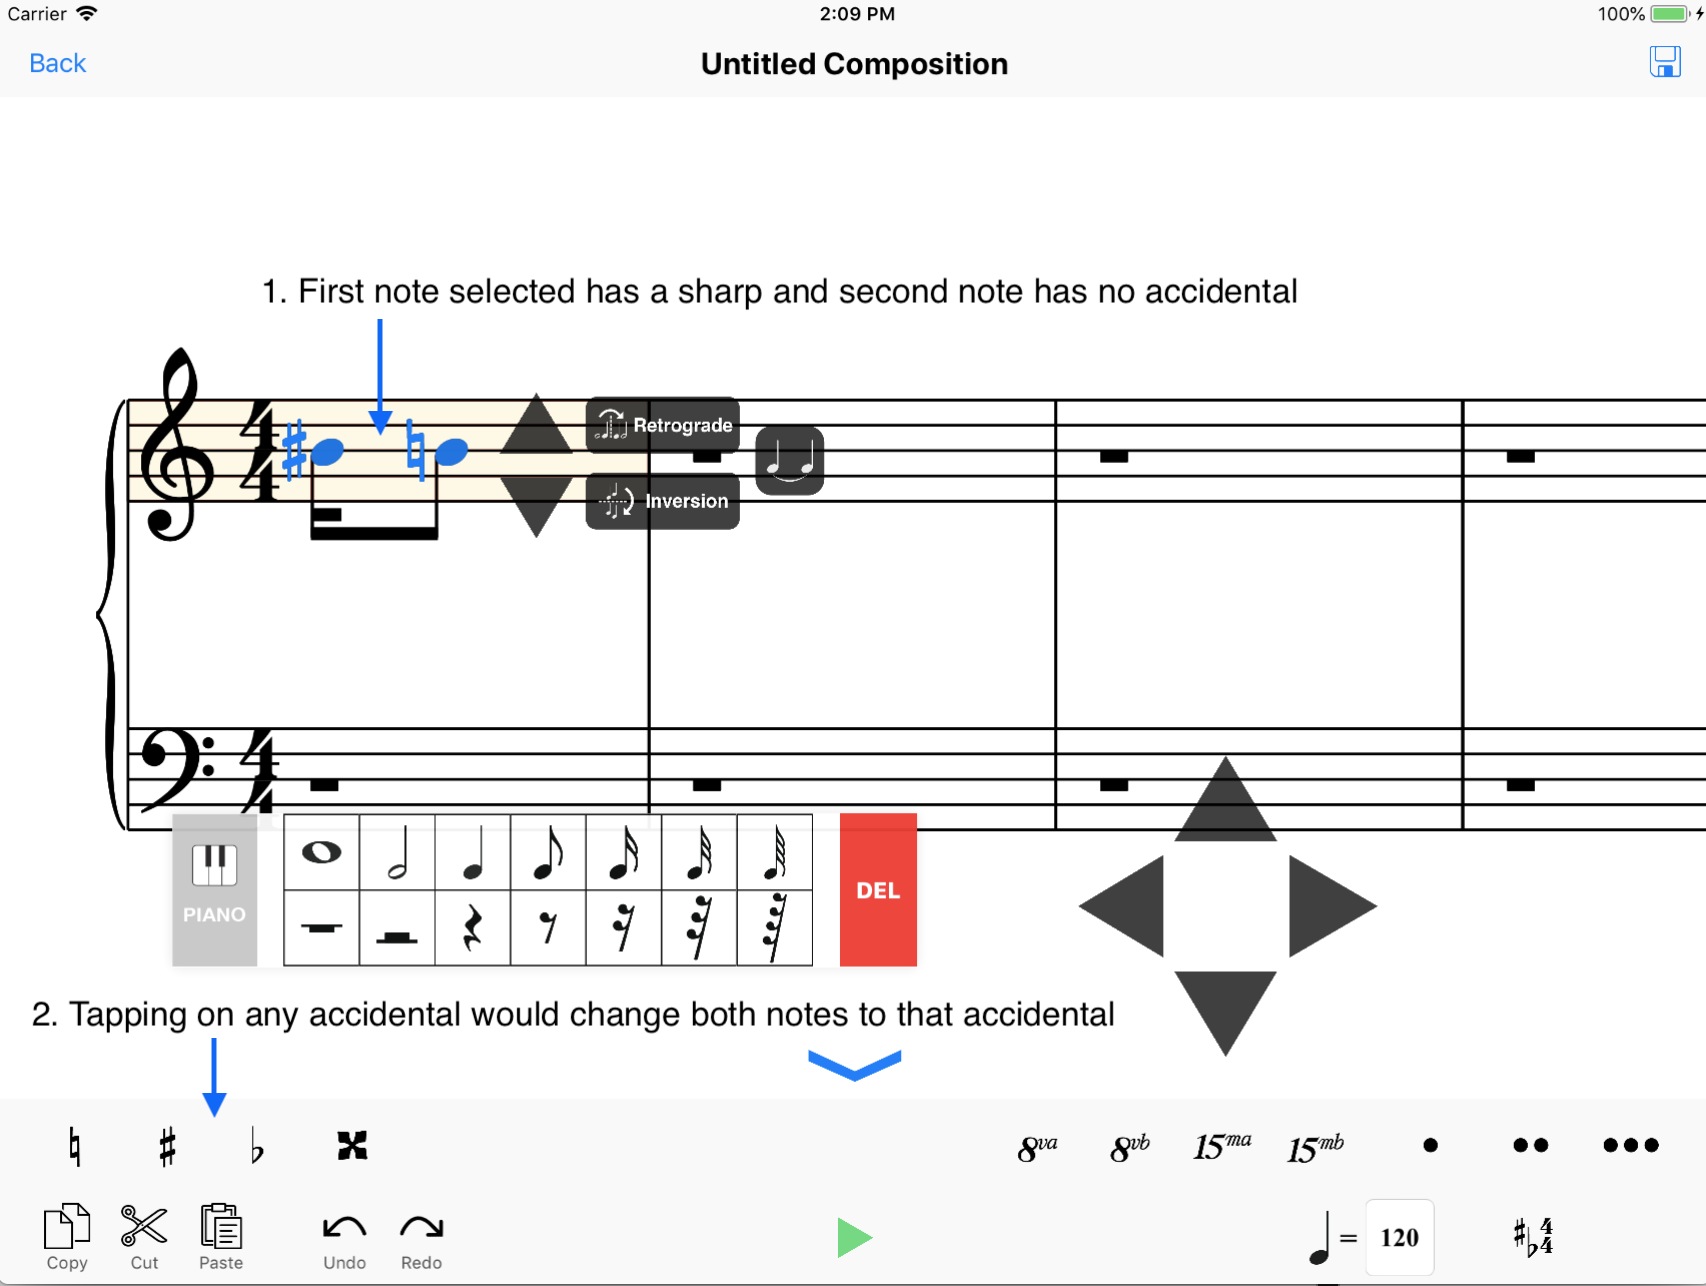
\includegraphics[scale=0.5]{Change_Accidental_Notes}
    \caption{Changing accidental on multiple notes with different accidentals.}
    \label{fig:change-accidental-notes}
\end{figure}

Removing accidentals, on the other hand, works by selecting a note with an accidental and tapping the same accidental again. When a single note with accidental is selected, the corresponding accidental button type would highlight blue in the bottom menu and the user may tap it to remove the accidental on the selected note (Figure \ref{fig:remove-note-accidental}).

\begin{figure}[H]
  \centering
  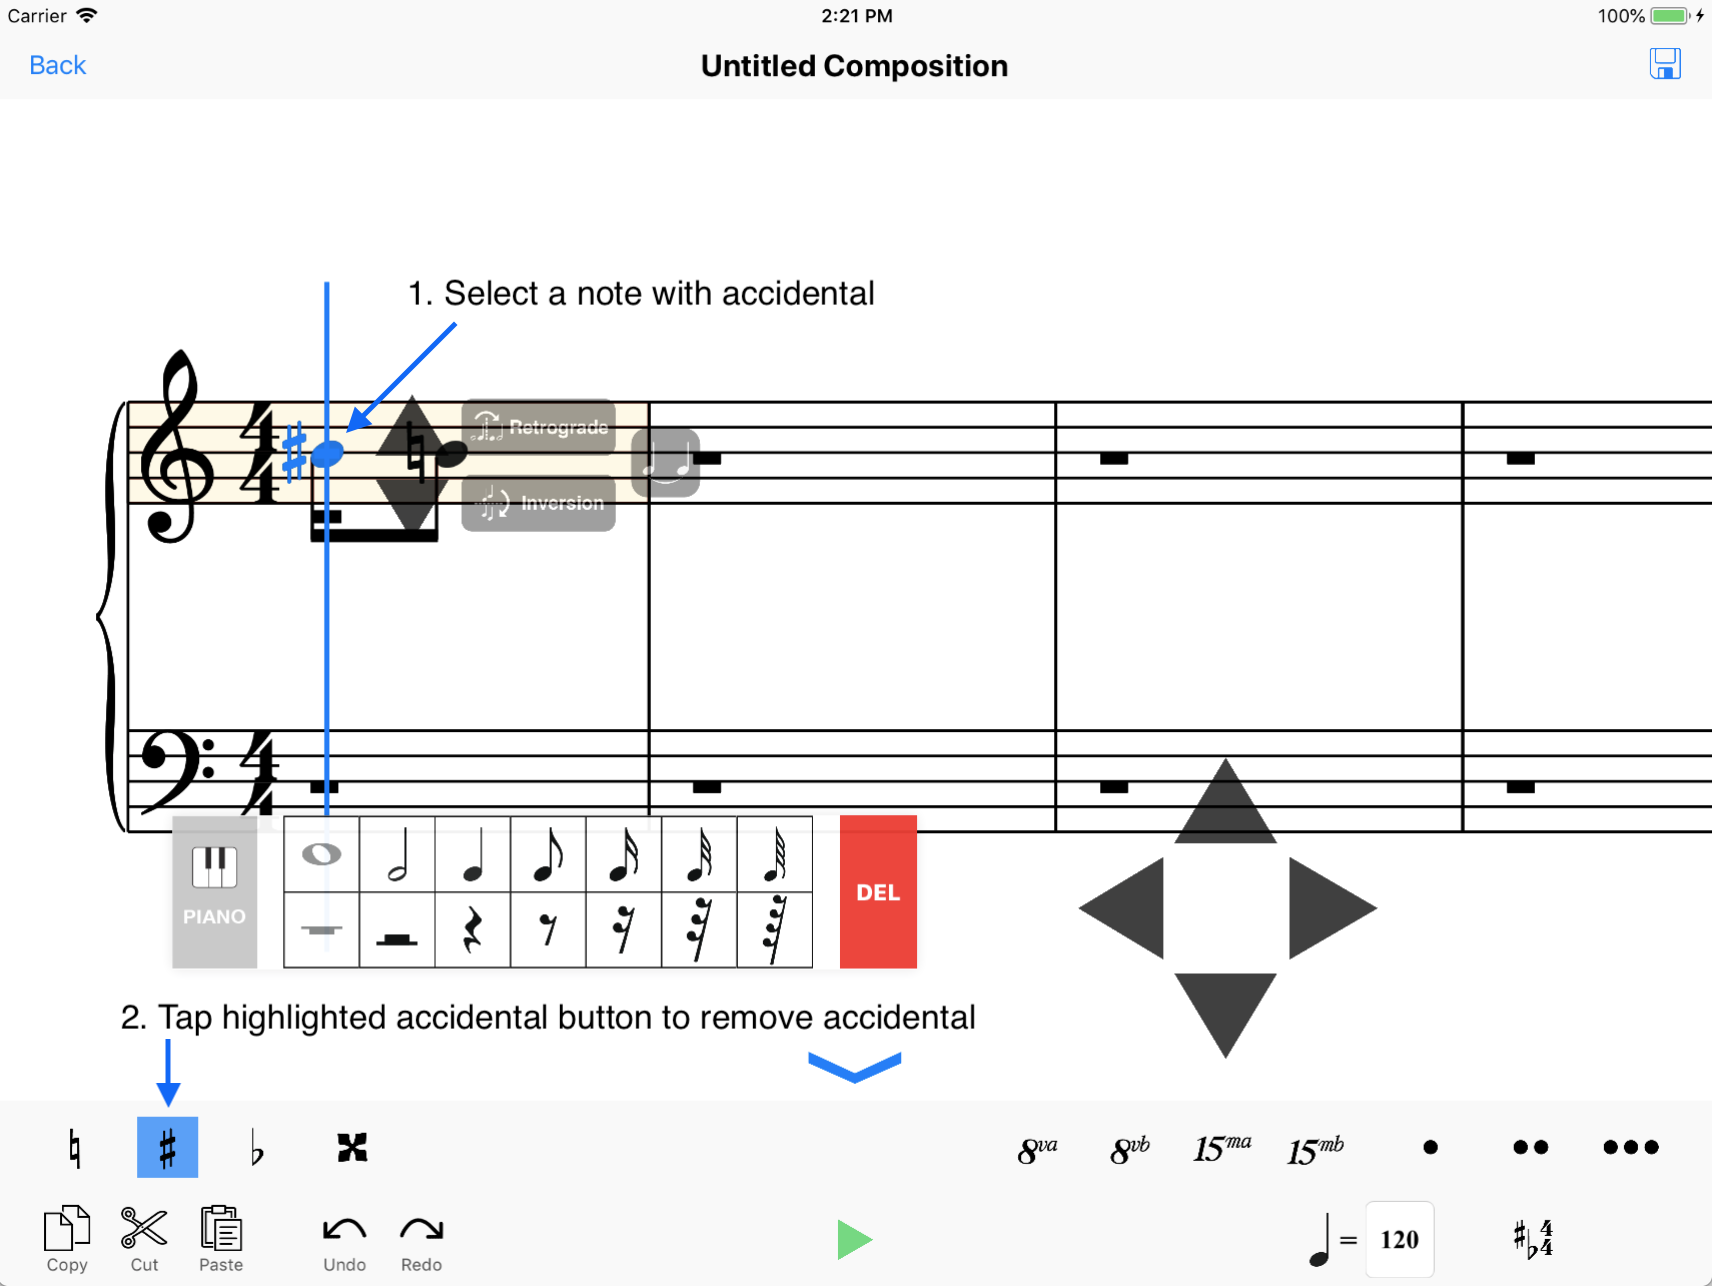
\includegraphics[scale=0.5]{Remove_Note_Accidental}
    \caption{Removing a note accidental.}
    \label{fig:remove-note-accidental}
\end{figure}

There is an alternative way of placing accidentals. This is done by tapping on any accidental button where there is no selected note. When an accidental button is highlighted and no note is selected, all notes that are added will automatically have the accidental selected. To unselect an accidental type, simply place the cursor where there is no note or rest again and tap the highlighted accidental button (Figure \ref{fig:alt-accidental}).

\begin{figure}[H]
  \centering
  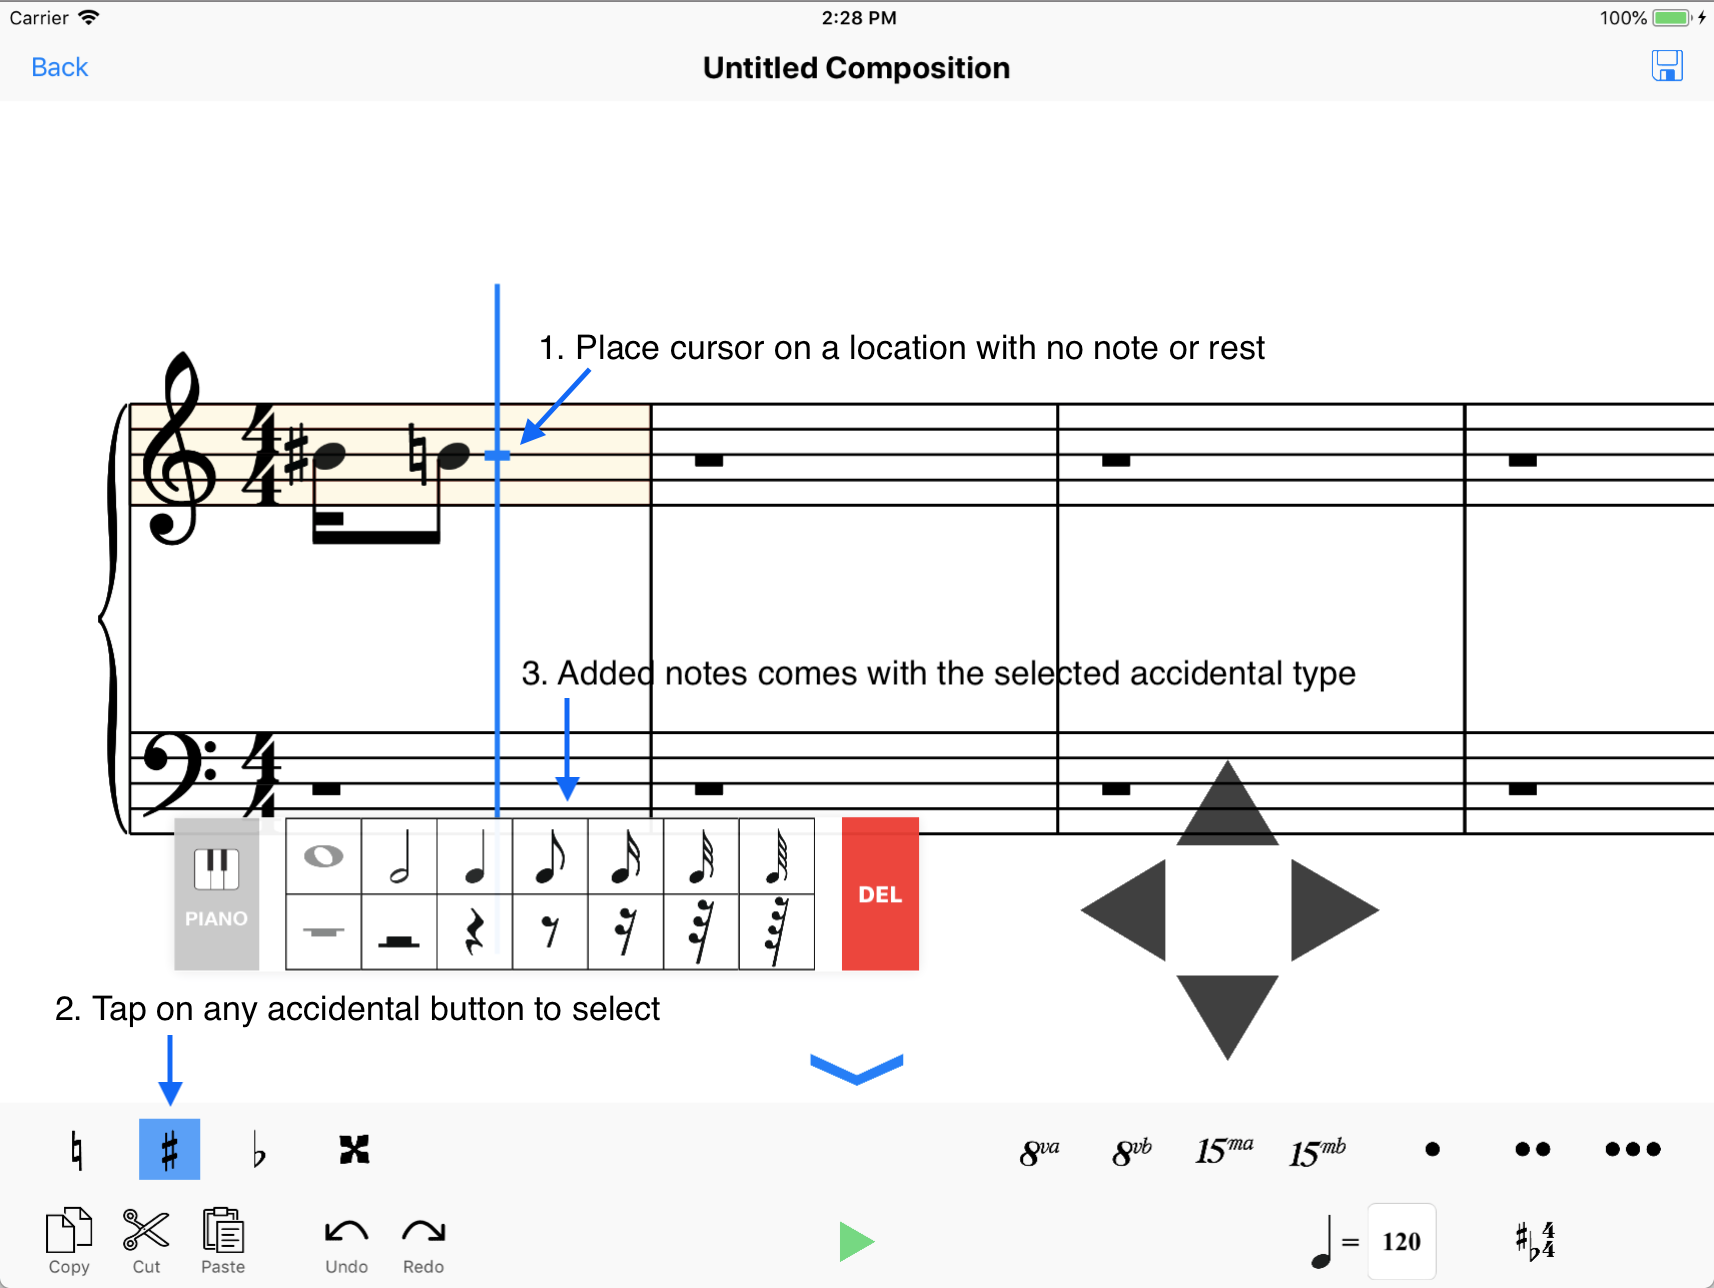
\includegraphics[scale=0.5]{Alt_Accidental}
    \caption{Alternative accidental input.}
    \label{fig:alt-accidental}
\end{figure}

The same behavior is implemented for adding and removing ottava and dots.

\section{Copying, Cutting, and Pasting Notes or Rests}
To copy or cut notes, the user must select the notes first and then tap on the copy or cut button in the bottom menu. After copying or cutting the notes, the user may then tap on the paste button to paste the notes on the location of the cursor (Figure \ref{fig:copy-cut-paste}).

\begin{figure}[H]
  \centering
  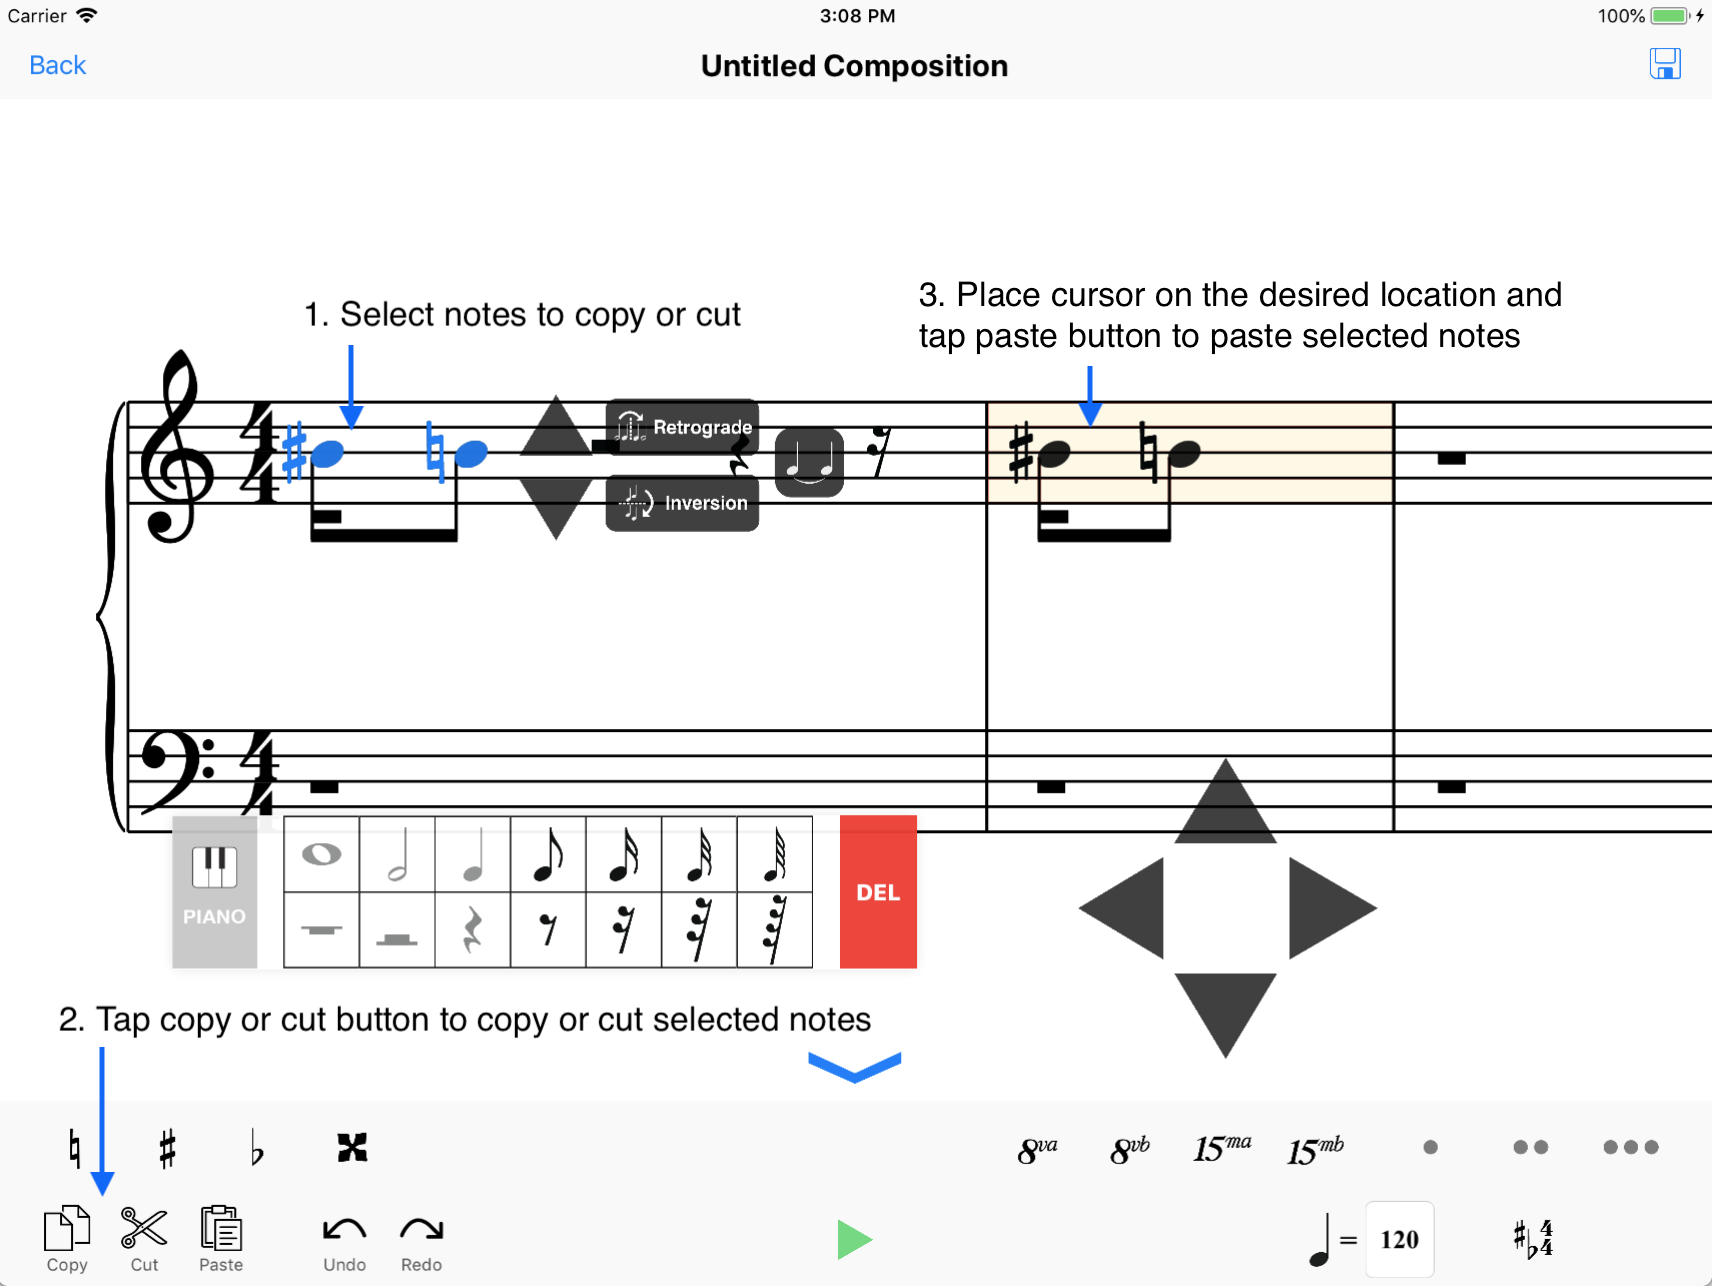
\includegraphics[scale=0.5]{Copy__Cut__Paste}
    \caption{Copying, cutting, and pasting notes.}
    \label{fig:copy-cut-paste}
\end{figure}

\section{Undoing and Redoing Actions}
To undo or redo an action, the user must tap on the undo or redo button in the bottom menu (Figure \ref{fig:undo-redo}).

\begin{figure}[H]
  \centering
  
\includegraphics[scale=0.8]{Undo_Redo}
    \caption{Undoing or Redoing actions.}
    \label{fig:undo-redo}
\end{figure}

\section{Changing the Tempo}
There are two ways of changing the tempo of a composition. The first way is by tapping on the tempo icon in the bottom right part of the menu, and the slider will appear allowing the user to slide it to the left or to the right whilst increasing or decreasing the tempo, respectively (Figure \ref{fig:tempo-slider}). Tapping anywhere outside the tempo slider would hide it.

\begin{figure}[H]
  \centering
  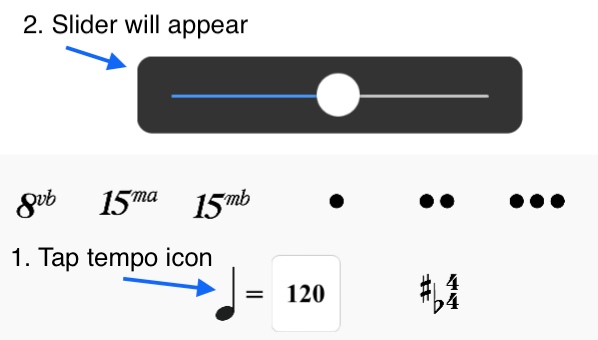
\includegraphics[scale=0.8]{Change_Tempo1}
    \caption{Changing the tempo using a slider.}
    \label{fig:tempo-slider}
\end{figure}

The second way of changing the tempo is by simply tapping on the textbox beside the tempo icon which allows the user to type in the desired tempo (Figure \ref{fig:tempo-type}).

\begin{figure}[H]
  \centering
  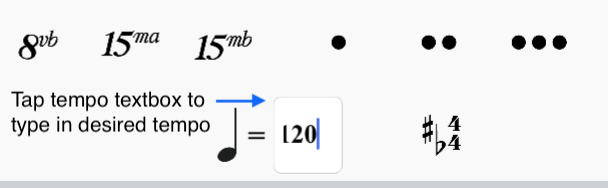
\includegraphics[scale=0.8]{Change_Tempo2}
    \caption{Changing the tempo by typing in the textbox.}
    \label{fig:tempo-type}
\end{figure}

\section{Changing Time Signature and Key Signature}
To change the time signature and key signature of the composition, the user must tap on the time / key signature button (Figure \ref{fig:tim-sig-btn}) on the bottom right part of the menu.

\begin{figure}[H]
  \centering
  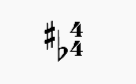
\includegraphics[scale=1]{Time_Sig_Btn}
    \caption{Time / Key Signature Button.}
    \label{fig:tim-sig-btn}
\end{figure}

After tapping the time / key signature button, a menu will appear which lets the user set both the time signature and key signature (Figure \ref{fig:tim-sig-menu}). To edit the time signature, the user may tap on one of the preset buttons which will set the values of the number of beats and beat duration automatically. Alternatively, the user may may manually enter the values for the number of beats and beat duration by tapping on their corresponding textboxes. Upon saving the changes of the new time signature, the notes inside the measures that are affected by the change will automatically readjust their location depending on the newly set time signature. In changing the key signature, the user may tap on one of the circular buttons for the key signature. After saving, changes will also affect the notes inside the affected measures.

\begin{figure}[H]
  \centering
  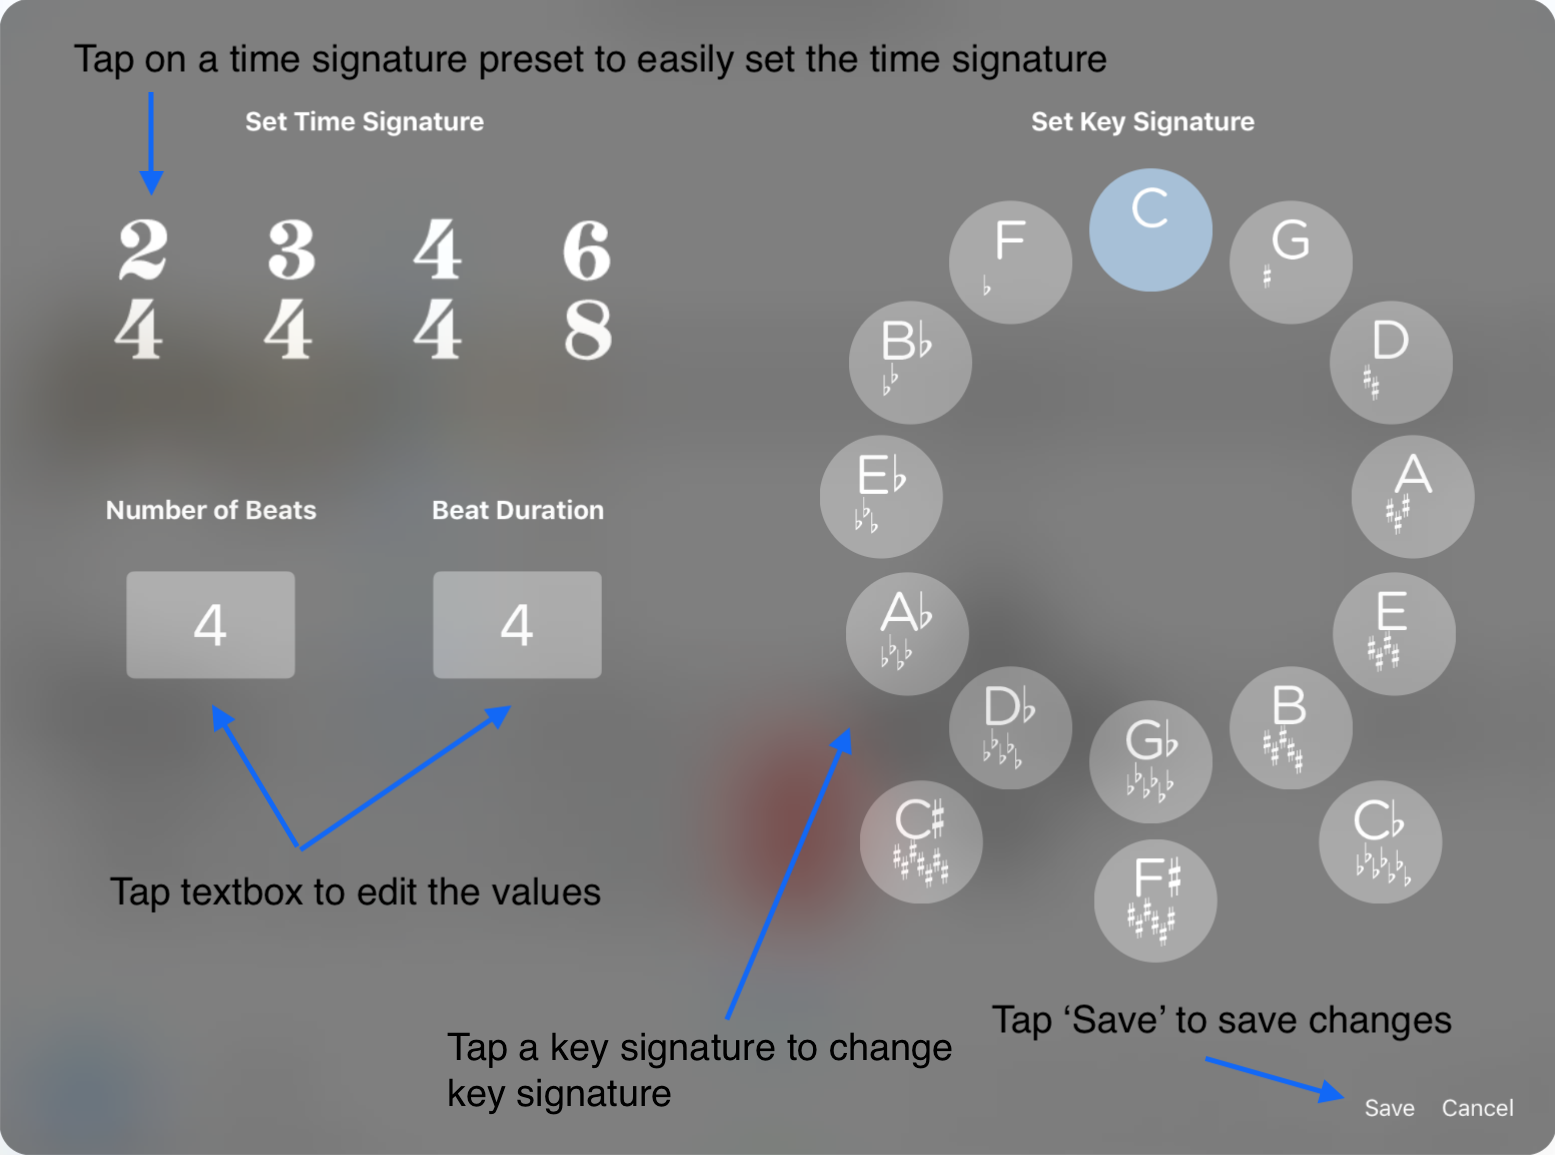
\includegraphics[scale=0.5]{Time_Sig_Menu}
    \caption{Time / Key Signature Menu.}
    \label{fig:tim-sig-menu}
\end{figure}

\section{Using the Keyboard for Note Input}
The application does not only allow users to add notes through the notation controls, but there is also an alternative way to add notes through the virtual keyboard. To activate the keyboard input, the user must tap on the keyboard button in the left side of the notation controls which brings out the virtual keyboard interface (Figure \ref{fig:keyboard}). After activating the keyboard input, the user may tap on a note type in the notation controls to change the type of note that will be added when pressing a key in the keyboard. Upon pressing a key in the keyboard, the note will be added on the location of the cursor with the corresponding pitch that was pressed on the keyboard and also the selected note type from the notation controls. To deactivate the keyboard input, the user must simply tap on the keyboard button again to hide the keyboard interface and go back to the original method of input.

\begin{figure}[H]
  \centering
  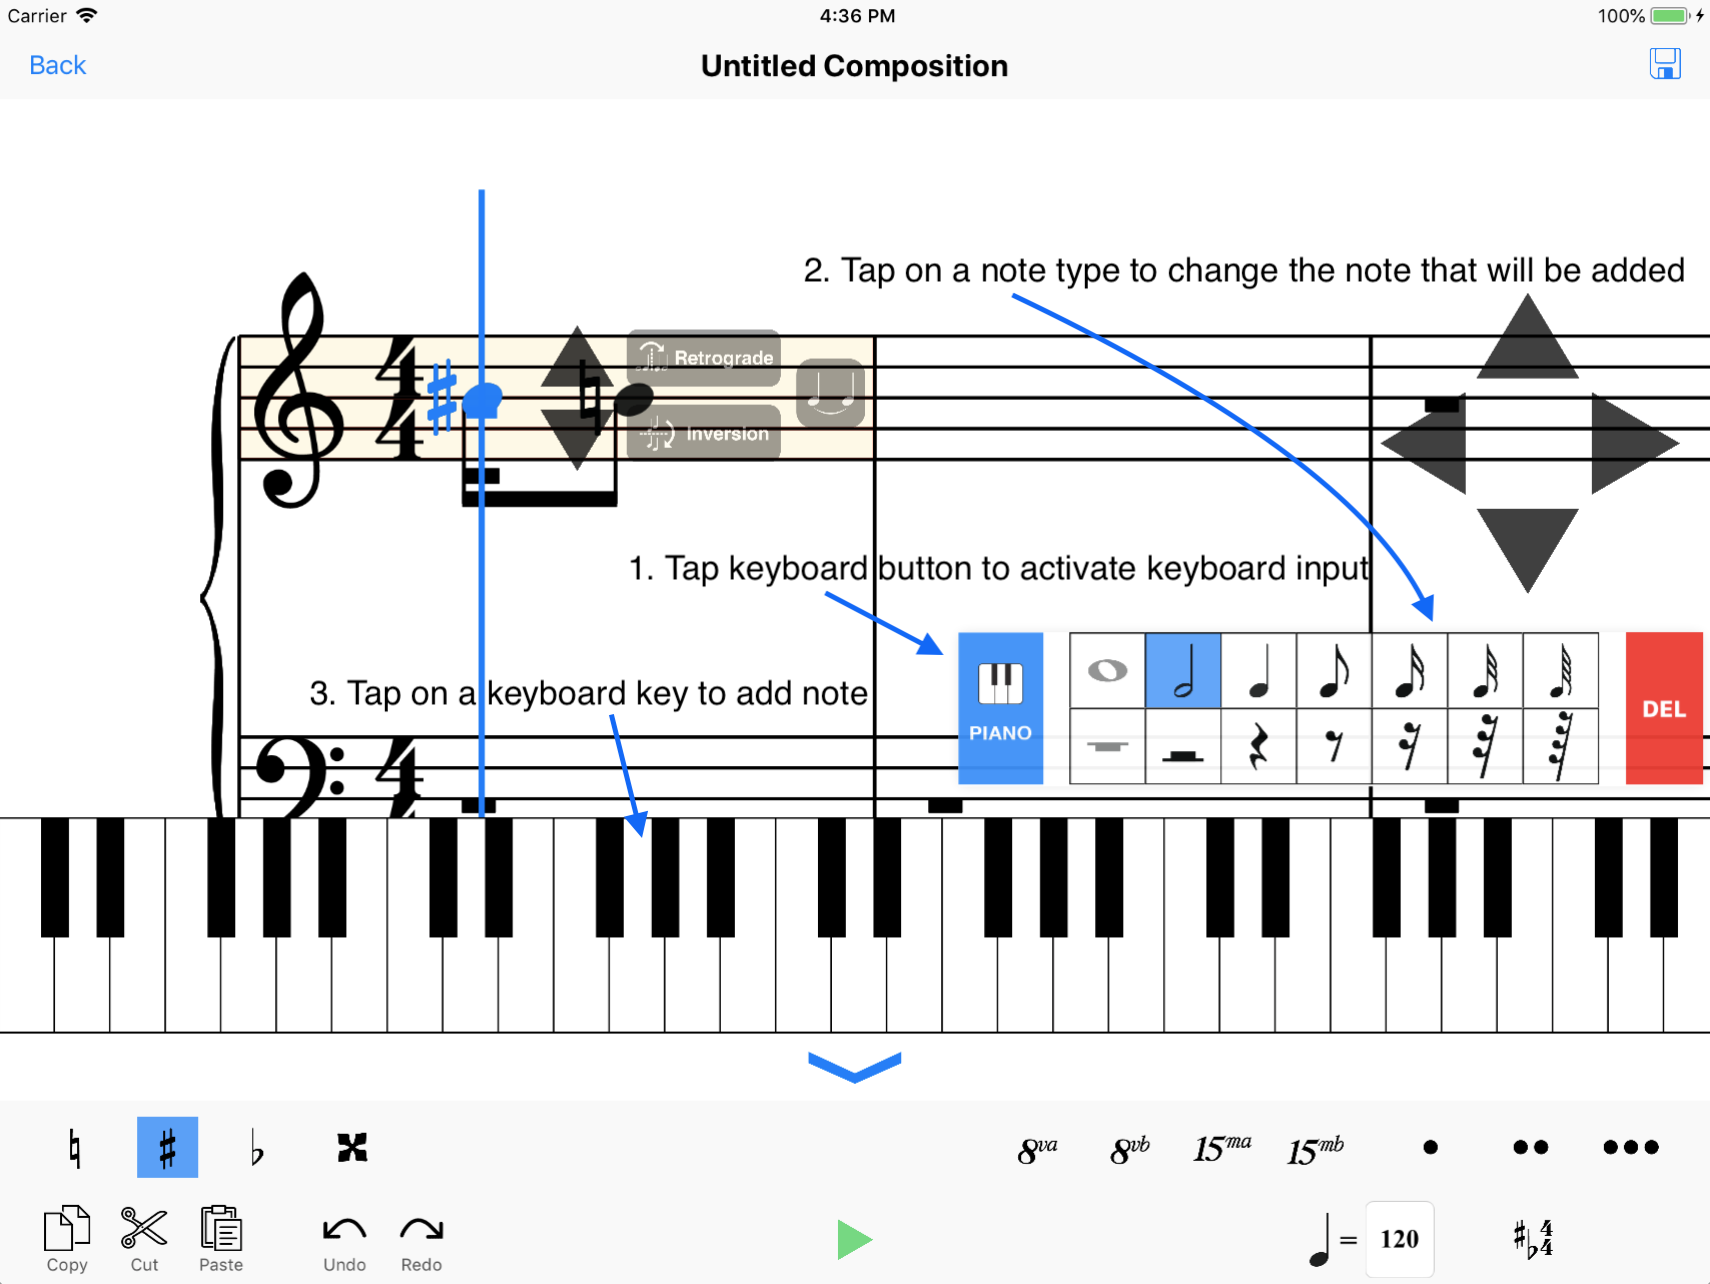
\includegraphics[scale=0.5]{Keyboard}
    \caption{Keyboard input.}
    \label{fig:keyboard}
\end{figure}

\section{Playing the Composition}
To play the composition, the user must simply tap on the play button on the bottom menu. Playback starts on the currently selected measure and note. The currently selected measure is the measure highlighted with yellow (Figure \ref{fig:play}).

\begin{figure}[H]
  \centering
  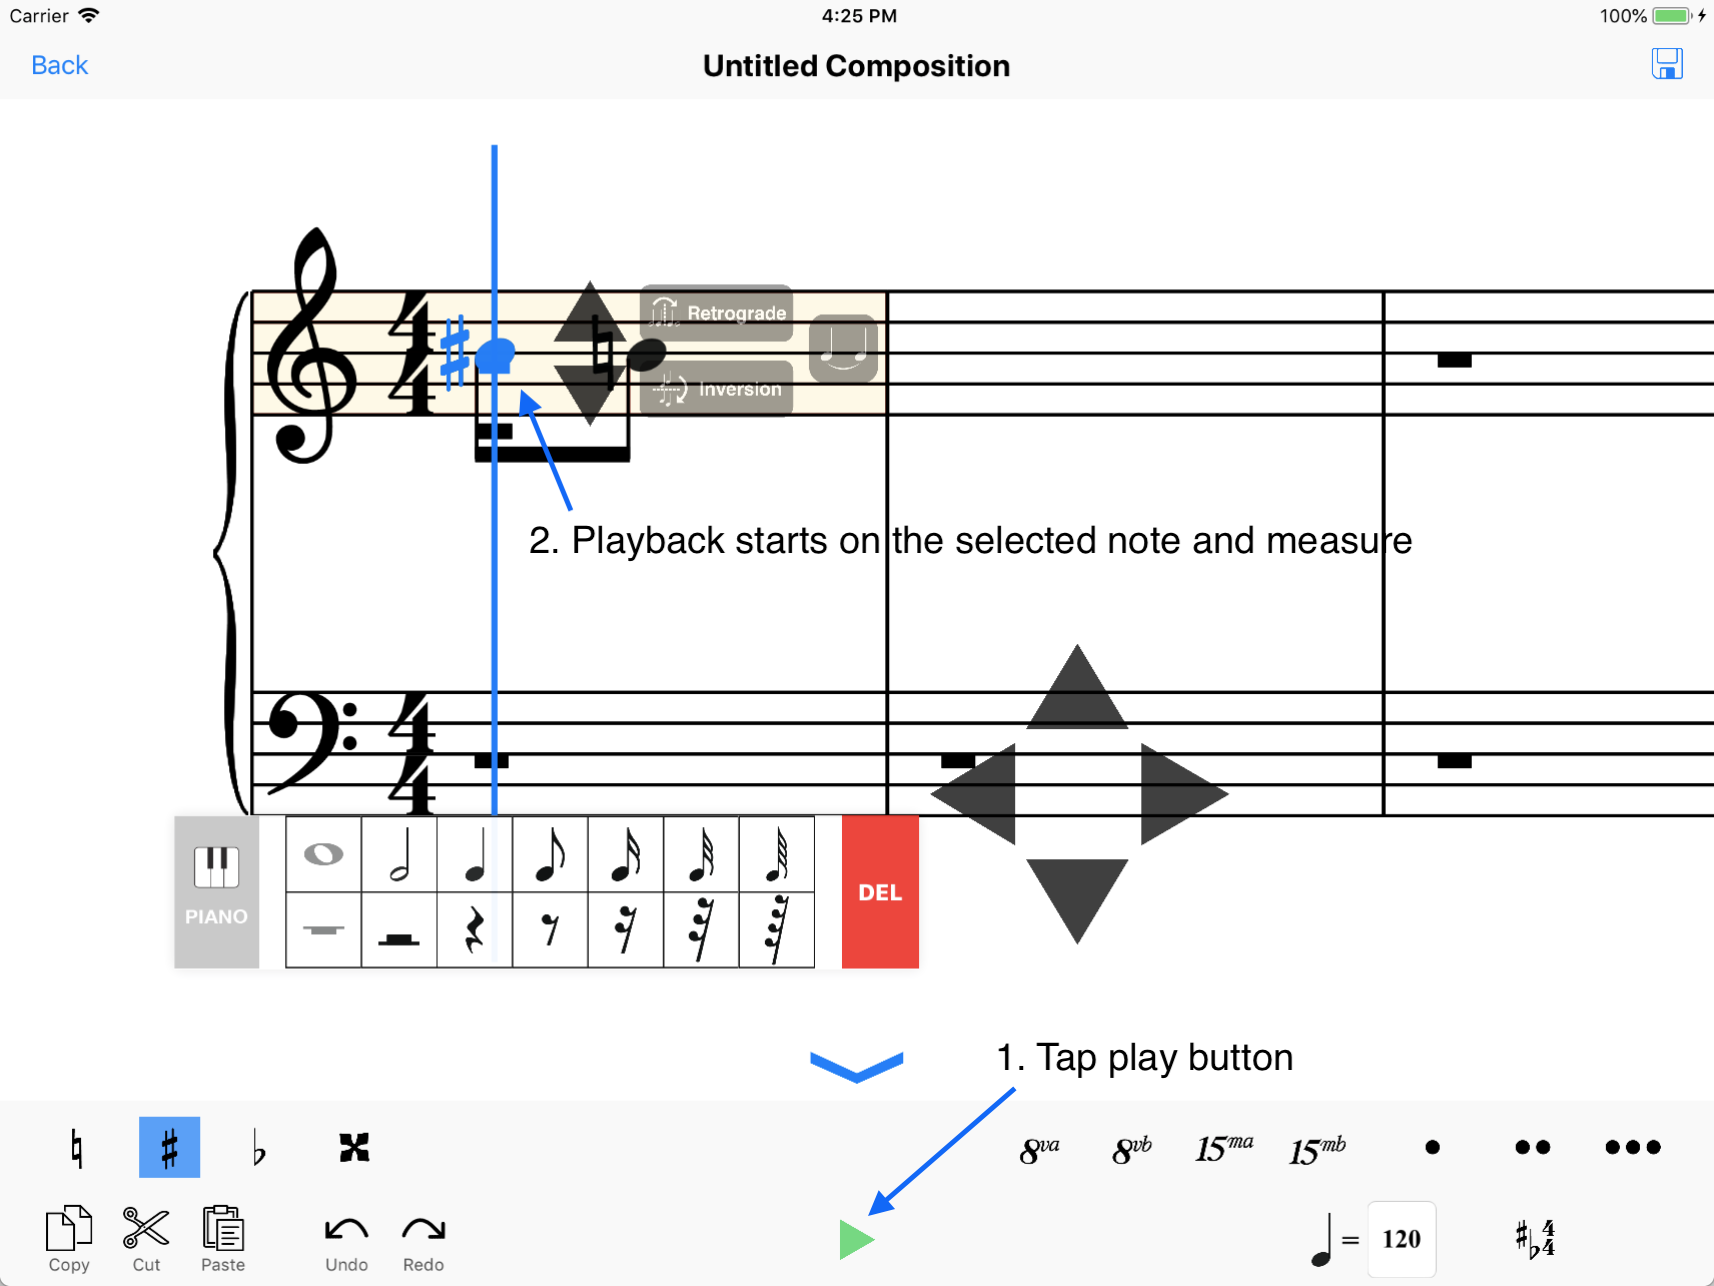
\includegraphics[scale=0.5]{Play}
    \caption{Playing the composition.}
    \label{fig:play}
\end{figure}

\section{Saving the Composition}
To save the composition, the user must simply tap on the save button in the upper right corner of the toolbar (Figure \ref{fig:save}).

\begin{figure}[H]
  \centering
  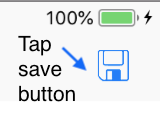
\includegraphics[scale=2]{Save}
    \caption{Saving the composition.}
    \label{fig:save}
\end{figure}

\section{Hiding and Showing the Bottom Menu}
To hide the bottom menu, the user must simply tap the arrow facing down on top of the bottom menu (Figure \ref{fig:hide}). To show it back again, the user must tap the arrow key facing up (Figure \ref{fig:show}).

\begin{figure}[H]
  \centering
  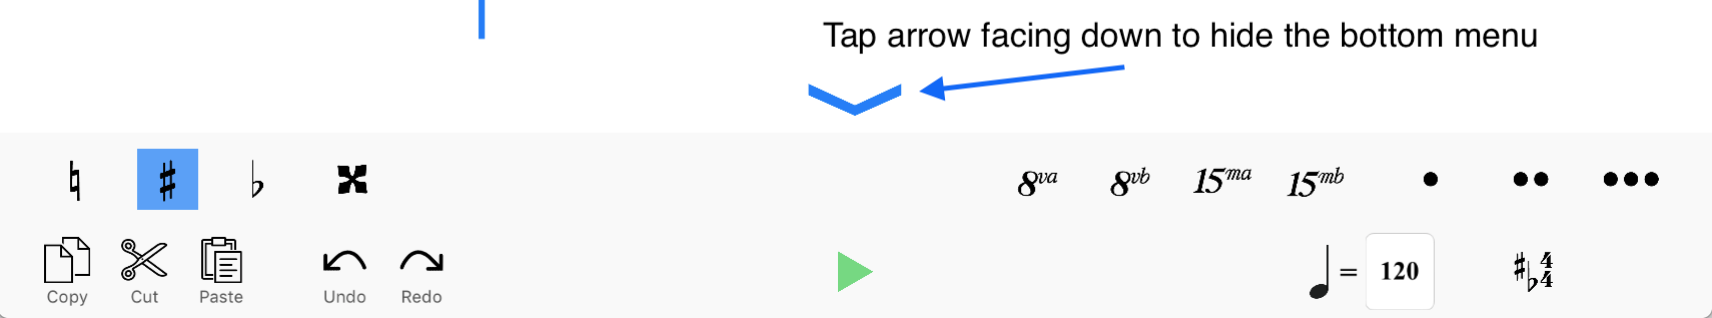
\includegraphics[scale=0.5]{Hide}
    \caption{Hiding the bottom menu.}
    \label{fig:hide}
\end{figure}

\begin{figure}[H]
  \centering
  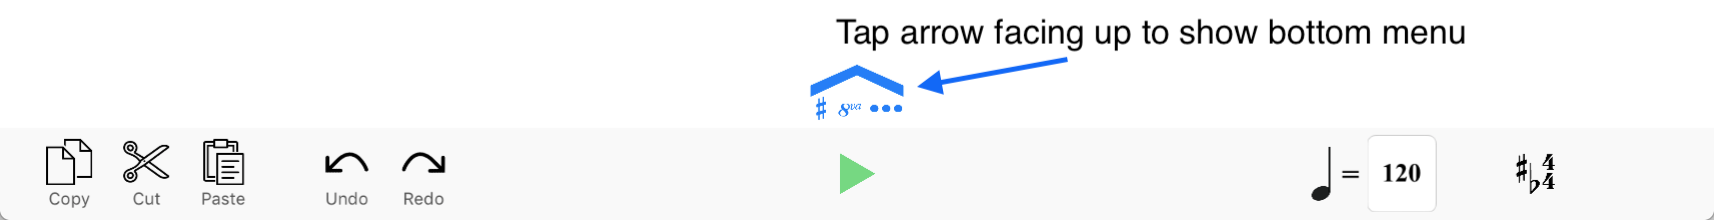
\includegraphics[scale=0.5]{Show}
    \caption{Showing the bottom menu.}
    \label{fig:show}
\end{figure}

\begin{comment}
\chapter{Initial Results}
\label{sec:appendixf}

\begin{longtable}{|p{5cm}|p{6cm}|p{1.5cm}|}
\caption{Motor Module} \label{tab:motor-module} \\
\hline

Attribute & Attribute Description & Value \\ \hline

PECK-FITTS-COEFF & b coefficient in Fitts's equation for PECK movements. & 0.075 \\ \hline

DEFAULT-TARGET-WIDTH & Effective width, in degrees visual angle, of targets with undefined widths. & 1.0 \\ \hline

MIN-FITTS-TIME & Minimum movement time for an aimed [Fitts's] movement. & 0.1  \\ \hline

MOTOR-BURST-TIME & Minimum time for any movement. & 0.05 \\ \hline

MOTOR-INITIATION-TIME & Time to initiate a motor movement. & 0.05 \\ \hline

MOTOR-FEATURE-PREP-TIME & Time to prepare a movement feature. & 0.001 \\ \hline

\end{longtable}

\begin{longtable}{|p{5cm}|p{6cm}|p{1.5cm}|}
\caption{Imaginal Module} \label{tab:imaginal-module} \\
\hline

Attribute & Attribute Description & Value \\ \hline

IMAGINAL-DELAY & Time in seconds to respond to an imaginal request & 0.2 \\ \hline

\end{longtable}

\begin{longtable}{|p{5cm}|p{6cm}|p{1.5cm}|}
\caption{Temporal Module} \label{tab:temporal-module} \\
\hline

Attribute & Attribute Description & Value \\ \hline

TIME-NOISE & Temporal noise & 0.015 \\ \hline

TIME-MASTER-START-INCREMENT & Temporal start interval & 0.011 \\ \hline

TIME-MULT & Temporal multiplier & 1.1 \\ \hline

RECORD-TICKS & Record each time increment as a buffer event & T \\ \hline

\end{longtable}

\end{comment}